\documentclass{article}
\usepackage[utf8]{inputenc}
\usepackage[margin=1in]{geometry}
\usepackage{hyperref}
\usepackage{setspace}
\pagenumbering{arabic}
\usepackage{graphicx}
\usepackage[dvipsnames]{xcolor}
\usepackage{fancyhdr} 
\usepackage{amsmath, amsfonts, amsthm, amssymb}
\usepackage{bbm}
\usepackage{nth}
\usepackage{dsfont}
\usepackage{subfig}
\usepackage{tikz}
\usepackage{accents}


% commenting
\newcommand{\comment}[3]{\textcolor{#1}{\textbf{[#2: }\textit{#3}\textbf{]}}}
\newcommand{\emma}[1]{\comment{purple}{EK}{#1}}
\newcommand{\jesse}[1]{\comment{BurntOrange}{JG}{#1}}
\newcommand{\miaoshiqi}[1]{\comment{ForestGreen}{ML}{#1}}
\newcommand{\siyue}[1]{\comment{blue}{SY}{#1}}

%For references using Lemma, Theorem, etc, use \cref
\usepackage[nameinlink,capitalize,sort]{cleveref}

% theorems
\newtheorem{theorem}{Theorem}[section]
\newtheorem{lemma}[theorem]{Lemma}
\newtheorem{definition}[theorem]{Definition}
\newtheorem{proposition}[theorem]{Proposition}
\newtheorem{example}[theorem]{Example}
\newtheorem{corollary}[theorem]{Corollary}
%theoremstyle{plain} %boldface title, italicized body. Commonly used in theorems, lemmas, corollaries, propositions and conjectures.
%\theoremstyle{definition} %boldface title, Roman body. Commonly used in definitions, conditions, problems and examples
\theoremstyle{remark} %italicized title, Roman body. Commonly used in remarks, notes, annotations, claims, cases, acknowledgments and conclusions.
\newtheorem{exercise}[theorem]{Exercise}

\newenvironment{solution}
  {\renewcommand\qedsymbol{$\blacksquare$}\begin{proof}[Solution]}
  {\end{proof}}

% weird hack to get rid of dot:
\usepackage{xpatch}
\makeatletter
\AtBeginDocument{\xpatchcmd{\@thm}{\thm@headpunct{.}}{\thm@headpunct{}}{}{}}



% lin alg
\newcommand{\bu}{{\mathbf{u}}}
\newcommand{\bv}{{\mathbf{v}}}
\newcommand{\bw}{{\mathbf{w}}}
\newcommand{\bx}{\mathbf{x}}
\newcommand{\zerovec}{{\mathbf{0}}}

% other useful stuff
\newcommand{\Id}{{\mathds{1}}}
\newcommand{\N}{{\mathbb{N}}}
\newcommand{\R}{{\mathbb{R}}}
\newcommand{\C}{{\mathbb{C}}}
\newcommand{\Z}{{\mathbb{Z}}}
\newcommand{\Q}{{\mathbb{Q}}}
\newcommand{\F}{{\mathbb{F}}}
\newcommand{\cL}{{\mathcal{L}}}
\newcommand{\cP}{\mathcal{P}}
\newcommand{\inv}{{-1}}

%\DeclareMathOperator{\dim}{dim}
\DeclareMathOperator{\range}{range}
\DeclareMathOperator{\rank}{rank}
\DeclareMathOperator{\nullity}{nullity}

\hypersetup{
  colorlinks   = true, %Colours links instead of boxes
  urlcolor     = blue, %Colour for external hyperlinks
  linkcolor    = black, %Colour of internal links
  citecolor   = black %Colour of citations
}

\allowdisplaybreaks % fixes align environment weird spacing on page
\setlength{\parindent}{0cm}
\usepackage[parfill]{parskip}

% get rid of dot after theorem 
\usepackage{xpatch}
\makeatletter
% Patch to accommodate for \begin{theorem}[...]
\AtBeginDocument{\xpatchcmd{\cref@thmoptarg}{\thm@headpunct{.}}{\thm@headpunct{}}{}{}}
% Patch to accommodate \begin{theorem} (without an optional argument)
\AtBeginDocument{\xpatchcmd{\cref@thmnoarg}{\thm@headpunct{.}}{\thm@headpunct{}}{}{}}

% \usepackage[natbib=true, style=vancouver]{biblatex}
\usepackage[backend= biber, style=alphabetic]{biblatex}
 %\usepackage{natbib}
 %\setcitestyle{square}
\bibliography{references.bib}

\title{Mathematics Bootcamp Lecture Notes \\
\vspace{0.5em}
\large Department of Statistical Sciences, University of Toronto}
\author{Emma Kroell}
\date{Last updated: \today}

\begin{document}

\maketitle


\newpage
\section*{Preface}

These lecture notes were prepared for the Operational Mathematics course at the Department of Statistical Sciences Graduate Student Bootcamp at the University of Toronto, held in July 2022 and July 2023. The course teaches an overview of necessary mathematics prerequisites to incoming statistics graduate students, with an emphasis on proofs.


These lectures are based on the following books:

1. \href{https://link-springer-com.myaccess.library.utoronto.ca/book/10.1007/978-1-4614-4265-3}{{\emph{An Introduction to Mathematical Structures and Proofs}}} by Larry J. Gerstein \\
2. \href{https://bookstore.ams.org/amstext-26/}{{\emph{The Tools of Mathematical Reasoning}}} by Tamara J. Lakins \\
3. \href{https://link-springer-com.myaccess.library.utoronto.ca/book/10.1007/0-387-28387-0}{\emph{A Taste of Topology}} by Volker Runde \\
4. \href{https://link-springer-com.myaccess.library.utoronto.ca/book/10.1007/978-3-319-17771-7}{\emph{Real Mathematical Analysis}} by Charles C. Pugh \\
5. \href{https://link-springer-com.myaccess.library.utoronto.ca/book/10.1007/978-3-319-11080-6}{{\emph{Linear Algebra Done Right}}} by Sheldon Axler \\
6. \href{https://www.math.brown.edu/streil/papers/LADW/LADW.html}{{\emph{Linear Algebra Done Wrong}}} by Sergei Treil 

Chapter 1 of Gerstein (2012) and the first three chapters of Lakins (2016) are used as references for the proof technique section. Runde (2005) is the main text for the sections on set theory, metric spaces, and topology, which follow chapters 1, 2, and 3 of his book, respectively. Some additional topics come from Pugh (2015). The linear algebra content comes mostly from Axler (2015), with Treil (2017) used in some sections for an alternate perspective, particularly for the content on determinants and spectral theory. The content on differentiation and integration is based on Chapter 3 of Pugh (2015). A few other texts and lecture notes are used at certain points, and are cited in the references section corresponding to that chapter.

Most of the material in these notes belongs to these texts. Many of these texts are available online to University of Toronto users (some to everyone).

I would like to acknowledge the assistance of Jesse Gronsbell, Stanislav Volgushev, Piotr Zwiernik, and Robert Zimmerman in developing the list of topics for the course. 

Please notify me of any typos or corrections at emma.kroell@mail.utoronto.ca.


\newpage
\tableofcontents


\newpage

{\bf A short note on notation: }

\vspace{0.5em}

$\N$ denotes the whole numbers, i.e. $\N = \{1,2,\ldots \}$

$\N_0$ denotes the non-negative integers, i.e. $\N_0 = \{0, 1,2,\ldots \}$

$\Z$ denotes the integers, i.e. $\Z = \{ \ldots, -2,-1,0,1,2,\ldots \}$

$\Q$ denotes the rational numbers, i.e. $\Q = \{ \frac{p}{q} \, | \, p, q \in \Z \text{ and } q \neq 0 \}$

$\R$ denotes the real numbers

$\C$ denotes the complex numbers



\section{Review of proof techniques}
\subsection{Propositional logic}

\emph{Propositions} are statements that could be true or false. They have a corresponding \emph{truth value}. We will use capital letters to denote propositions. For example, ``$n$ is odd'' and ``$n$ is divisible by 2'' are propositions. Let's call them $P$ and $Q$. Whether they are true or not (i.e. their truth value) depends on what $n$ is. 

We can  negate statements: $\neg P$ is the statement ``$n$ is not odd''.

 We can combine statements: 
 \begin{itemize}
 \item $P \wedge Q$ is the statement ``$n$ is odd and $n$ is divisible by 2''.
 \item $P \vee Q$ is the statement ``$n$ is odd or $n$ is divisible by 2''.
\end{itemize}
We always assume the inclusive or unless specifically stated otherwise.


\begin{example}
Here are some statements, which we want to write in propositional logic.
\begin{itemize}
              \item If it's not raining, I won't bring my umbrella.
              \item I'm a banana or Toronto is in Canada.
              \item If I pass this exam, I'll be both happy and surprised.
\end{itemize}

For the first one, let $A$ be the statement ``it's raining'' and $B$ be the statement ``I will bring my umbrella''. In logic, the statement is $\neg A \implies \neg B$.

For the second, let $C$ be the statement ``I'm a banana'' and let $D$ be the statement ``Toronto is in Canada''. We write this as $C \vee D$.

For the third, let $P$ be the statement ``I pass this exam'', let $Q$ be the statement ``I am happy'', and let $R$ be the statement ``I am surprised''. This one is written $P \implies (Q \wedge R)$.
\end{example}

\subsubsection{Truth values}

\begin{example} Write the following using propositional logic: \\
If it is snowing, then it is cold out. \\
It is snowing. \\
Therefore, it is cold out.

Solution. \\
$P \implies Q$ \\
$P$ \\
Conclusion: $Q$ \\
\end{example}

To examine if a statement is true or not, we use a truth table, where we write out all the possibilities. 

\begin{example}
The truth table for $P \implies Q$ where $P$, $Q$ are propositions is:

\begin{tabular}{|c|c| c|}
\hline
     $P$& $Q$ &  $P \implies Q$ \\ \hline
     T& T & T \\ \hline
     T & F & F \\ \hline
     F & T & T \\ \hline
     F & F & T \\ \hline
\end{tabular}
\end{example}

\subsubsection{Logical equivalence}
We say that two statements are \emph{logically equivalent} if they have the same truth tables.

\begin{example}
\label{ex:implication_table}
Let $P$, $Q$ be propositions. $P \implies Q$ is logically equivalent to $\neg P \vee Q$.
 
 
\begin{tabular}{|c|c| c|}
\hline
     $P$& $Q$ &  $P \implies Q$ \\ \hline
     T& T & T \\ \hline
     T & F & F \\ \hline
     F & T & T \\ \hline
     F & F & T \\ \hline
\end{tabular} \hspace{2cm} \begin{tabular}{|c | c | c | c|}
\hline
     $P$& $Q$ & $\neg P$ & $\neg P \vee Q$  \\ \hline
     T& T & F & T \\ \hline
     T & F & F & F \\ \hline
     F & T &  T &T \\ \hline
     F & F & T & T \\ \hline
\end{tabular}
\end{example}

\vspace{1em}

\begin{theorem}[De Morgan's Laws]
\label{thm:demorgan}
Let $P$, $Q$ be propositions.
\begin{enumerate}
    \item[(i)] $\neg (P \wedge Q)$ is logically equivalent to $\neg P \vee \neg Q$.
    \item[(ii)] $\neg (P \vee Q)$ is logically equivalent to $\neg P \wedge \neg Q$.
\end{enumerate}
\end{theorem}

Proving this is your first exercise.

The following fact is often useful.
\begin{example}
\label{ex:ifthen}
$\neg (P \implies Q)$ is logically equivalent to $P \wedge \neg Q$. This follows from \cref{ex:implication_table} and \cref{thm:demorgan}.
\end{example}

\subsubsection{Quantifiers}
There are two important logical operators that we have not yet discussed. They are denoted using the following symbols: $\forall$, read as ``for all'' or ``for each'', and $\exists$, read as ``there exists''. We will explore their meanings, how they can help us simplify statements we need to prove, and how we prove such statements.

\textbf{For all}

``for all'', $\forall$, is also called the universal quantifier. If $P(x)$ is some property that applies to $x$ from some domain, then $\forall x P(x)$ means that the property $P$ holds for every $x$ in the domain. An example is the statement ``Every real number has a non-negative square.'' We write this as $\forall x \in \R, \, x^2 \geq 0$. In logic, people often use brackets to separate parts of the logical expression, ex. $(\forall x \in \R) (x^2 \geq 0)$.

How do we prove a for all statement? We need to take an arbitrary element of the domain, and show the property holds for that element.

\textbf{There exists}

``there exists'', $\exists$, is also called the existential quantifier. If $P(x)$ is some property that applies to $x$ from some domain, then $\exists x P(x)$ means that the property $P$ holds for some $x$ in the domain. An example is the statement that 4 has a square root in the reals. We write this as $\exists x \in \R$ such that $x^2 = 4$ or in proper logic notation, $(\exists x \in \R$) ($x^2 = 4)$.

How do we prove a there exists statement? We need to find an element in the domain for which the property holds (find an example).

There is also a special way of writing when there exists a unique element. We use $\exists!$ for this case. For example, the statement ``there exists a unique positive integer such that the integer squared is 64'' is written $\exists!  z \in \N$ such that $z^2 = 64$.

\textbf{Combining quantifiers}

Often we will need to prove statements where we combine quantifiers. Here are some examples:

\begin{tabular}{p{0.45\textwidth} p{0.45\textwidth}}
     Statement & Logical expression \\
     \hline
     Every non-zero rational number has a multiplicative inverse & $\forall q \in \Q \setminus \{0\}, \, \exists s \in \Q$ such that $qs=1$ \\
     Each integer has a unique additive inverse & $\forall x \in \Z \, , \exists ! y \in \Z$ such that $x+y = 0$ \\
     $f:\R \to \R$ is continuous at $x_0\in\R$ \ &  $\forall \epsilon >0 \; \exists \delta > 0$ such that whenever $|x - x_0| < \delta$, $|f(x)-f(x_0)| < \epsilon$
\end{tabular}

\vspace{1em}

The order of quantifiers is important! Changing the order changes the meaning. Consider the following example. Which are true? Which are false?

\begin{center}

$\forall x \in \R \, \forall y \in \R$  $x + y = 2$ \\
$\forall x \in \R \, \exists y \in \R$  $x + y = 2$ \\
$\exists x \in \R \, \forall y \in \R$  $x + y = 2$ \\
$\exists x \in \R \, \exists y \in \R$ $x + y = 2$ 
\end{center}
\vspace{1em}

It's also important to know how to negate logical statements that include quantifiers, as it will often help us prove or disprove the statements. The results are intuitive, but things can get complicated when we have more complex statements. The negation of a statement being true for all $x$ is that is isn't true for at least one $x$. The negation of a statement being true for at least one $x$ is that is isn't true for any $x$. 

In summary,

\begin{center}
    $\neg \forall x P(x)$ = $\exists  x (\neg P(x))$ \\
$\neg \exists x P(x)$ = $\forall x (\neg P(x))$
\end{center}

\vspace{1em}

The negations of the statements above are:
\vspace{1em}

\begin{tabular}{p{0.45\textwidth} p{0.45\textwidth}}
     Logical expression & Negation \\
     \hline
     $\forall q \in \Q \setminus \{0\}, \, \exists s \in \Q$ such that $qs=1$ & $\exists q \in \Q \setminus \{0\}$ such that  $\forall s \in \Q, \, qs \neq 1$\\
     $\forall x \in \Z \, , \exists ! y \in \Z$ such that $x+y = 0$ & $\exists x \in \Z$ such  that $(\forall y \in \Z, x+y \neq 0)$ $\vee$ $(\exists y_1, y_2 \in \Z$ such that $y_1 \neq y_2 \wedge x+y_1 = 0 \wedge x+y_2 = 0$  ) \\
     $\forall \epsilon >0 \; \exists \delta > 0$ such that whenever $|x - x_0| < \delta$, $|f(x)-f(x_0)| < \epsilon$ & $\exists \epsilon >0$ such that $\forall \delta > 0$,  $|x - x_0| < \delta$ and  $|f(x)-f(x_0)| \geq \epsilon$
\end{tabular}

\vspace{1em}

Note that we use De Morgan's laws (\cref{thm:demorgan}), as well as the negation of an implication (\cref{ex:ifthen}). What do these negations mean in English?


\subsection{Types of proof}

\subsubsection{Direct proof}

In a direct proof, our approach is to use the definition and known results.

\begin{example}
The product of an even number with another integer is even.
\end{example}

To prove this statement, we will use the definition of even. First we state that definition.

\begin{definition}
We say that an integer $n$ is \emph{even} if there exists another integer $j$ such that $n=2j$. \\
We say that an integer $n$ is \emph{odd} if there exists another integer $j$ such that $n=2j+1$.
\end{definition}

Now we prove the example directly.

\begin{proof}
Let $n, m \in \Z$, with $n$ even. By definition, there $\exists$ $j \in \Z$ such that $n = 2j$. Then 
$$ n m  =  (2 j) m = 2 (j m)$$
Therefore $n m$ is even by definition. 
\end{proof}

Here is another example, which uses the concept of divisibility.

\begin{definition}
Let $a,b \in \Z$. We say that ``a divides b'', written $a | b$, if the remainder is zero when $b$ is divided by $a$, i.e. $\exists j \in \Z$ such that $b = a j$.
\end{definition}

% https://hsm.stackexchange.com/questions/5656/who-invented-the-divisibility-symbol-and-why-is-it-backwards

\begin{example}
Let $a,b,c \in \Z$ with $a \neq 0$. Prove that if $a | b$ and $b | c$, then $a | c$.
\end{example}
\begin{proof}
Let $a,b,c \in \Z$. Suppose $a | b$ and $b | c$. Then by definition, there exists $j,k \in \Z$ such that $b = aj$ and $c = kb$. Combining these two equations gives $c = k (aj) = a (kj)$. Thus $a | c$ by definition.
\end{proof}


\subsubsection{Proof by contrapositive}
Sometimes instead of proving an implication $P \implies Q$ directly, it is easier to prove $\neg Q \implies \neg P$. This is called the contrapositive. First, we show that these two statements are logically equivalent using truth tables. 

$P \implies Q$  \hspace{5cm}  $\neg Q \implies \neg P$

        \vspace{1em}
\begin{tabular}{|c|c| c|}
\hline
     $P$& $Q$ &  $P \implies Q$ \\ \hline
     T& T & T \\ \hline
     T & F & F \\ \hline
     F & T & T \\ \hline
     F & F & T \\ \hline
\end{tabular}   \hspace{2cm}  \begin{tabular}{|c | c | c |  c | c |}
\hline
     $P$& $Q$ & $\neg P$ &  $\neg Q$ & $\neg Q \implies \neg P$ \\ \hline
     T& T & F & F & T \\ \hline
     T & F & F &  T & F \\ \hline
     F & T &  T  & F & T \\ \hline
     F & F & T & T & T \\ \hline
\end{tabular}
\vspace{1.5em}

Note that $\neg P \implies \neg Q$ is \emph{not} logically equivalent to  $P \implies Q$ (can you think of an example?). This is a common mistake.

Here is an example of a statement that is easier to prove using the contrapositive as opposed to directly.

\begin{example}
If an integer squared is even, then the integer is itself even.
\end{example}

\begin{proof}
We prove the contrapositive. Let $n$ be odd. Then there exists $k \in \Z$ such that $n = 2k + 1$. We compute
$$n^2 = (2k + 1)^2 = 4k^2 + 4k + 1 = 2(2k^2+2k) + 1.$$
Thus $n^2$ is odd.
\end{proof}


\subsubsection{Proof by contradiction}

Another proof technique is to assume something we know to be (or think to be) false, and then try to derive a contradiction. A contradiction is something that is impossible, like 0=1 or showing that a number is both odd and even. 

In sum, to prove that a statement $P$ is true by contradiction, we assume $\neg P$ is true, derive a contradiction, and conclude that $P$ is true. Here is an example.

\begin{example}
The sum of a rational number and an irrational number is irrational.
\end{example}

\begin{proof}
Let $q \in \mathbb{Q}$ and $r \in \mathbb{R} \setminus \mathbb{Q}$.
Suppose in order to derive a contradiction that their sum is rational, i.e. $ r + q = s$ where $s \in \mathbb{Q}$.
But then $r = s - q \in \mathbb{Q}$. Contradiction. Therefore the sum of a rational number and an irrational number is irrational.
\end{proof}


\subsubsection{Summary}

{\bf In sum, to prove $P \implies Q$:} 

\begin{tabular}{r l}
     Direct proof:  & assume $P$, prove $Q$ \\
     Proof by contrapositive:  & assume $\neg Q$, prove $\neg P$ \\ 
     Proof by contradiction: & assume $P \wedge \neg Q$ and derive something that is impossible \\ 
\end{tabular}

\vspace{0.5em}

\subsubsection{Induction}

Finally, we consider a special proof technique for proving statements about the natural numbers (or subsets of them of certain forms). It is based on the following theorem, which we state without proof. 

\begin{theorem}[Well-ordering principle for $\mathbb{N}$]
Every nonempty set of natural numbers has a least element.
\end{theorem}

Because of the well-ordering principle, we can prove something holds for the natural numbers by proving it holds for the smallest one, and then creating a logical ladder linking them together as follows:

\begin{theorem}[Principle of mathematical induction]
Let $n_0$ be a non-negative integer. Suppose $P$ is a statement about positive integers $n$ such that 
\begin{enumerate}
\item(base case) $P(n_0)$ is true 
\item (induction step) For every integer $k \geq n_0$, if $P(k)$ is true, then $P(k+1)$ is true.
\end{enumerate}
Then $P(n)$ is true for every integer $n \geq n_0$
\end{theorem}

Here is an example of a proof by induction.

\begin{example}
$n! > 2^n$ if $n \geq 4$.
\end{example}

\begin{proof}
We prove this by induction on $n$. \\
{\it Base case:} Let $n = 4$. Then $n! = 4! = 24 > 16 = 2^4$. \\
{\it Inductive hypothesis:} Suppose for some $k \geq 4$, $k! > 2^k$. \\
Then
$$(k+1)! = (k+1) k! > (k+1) 2^k > 2 (2^k) = 2^{k+1}.$$
Thus the statement holds by induction on $n$.
\end{proof}

Sometimes we use a different version of induction, called strong induction.  

\begin{theorem}[Principle of strong mathematical induction]
Let $n_0$ be a non-negative integer.  Suppose $P$ is a statement about positive integers $n$ such that
\begin{enumerate}
\item(base case) $P(n_0)$ is true 
\item (induction step) For every integer $k \geq n_0$, if $P(m)$ is true for every integer $m$ with $n_0 \leq m \leq k$, then $P(m+1)$ is true.
\end{enumerate}
Then $P(n)$ is true for every integer $n \geq n_0$.
\end{theorem}

Next, we will consider an example where it is much simpler to use the strong version of induction than the regular one. First, we recall the definition of a prime number.

\begin{definition}
\label{def:prime}
A positive integer $p$ is prime if $p$ has exactly two positive integer factors: 1 and $p$. Note that $1$ is not prime. We can write this as 
$$ p > 1 \text{ is prime if } \forall \, a, b \in \N, \, p=ab \implies (a = 1 \text{ or } b =1).$$
\end{definition}

We want to prove the existence part of the Fundamental Theorem of Arithmetic, that every integer greater than or equal to 2 has a prime factorization. The fact that such a factorization is unique is left as an exercise.

\begin{example}
Every integer $n \geq 2$ can be written as the product of primes.
\end{example}

\begin{proof}
We prove this using the Principle of Strong Mathematical Induction on $n$.

{\it Base case:} $n = 2$ is prime. 

{\it Inductive hypothesis:} Suppose for some $k \geq 2$ that one can write every integer $n$ such that $2 \leq n \leq k$ as a product of primes.

We must show that we can write $k+1$ as a product of primes.

{\it Case 1:} if $k+1$ is prime, then we are done. 

{\it Case 2:} if $k+1$ is not prime, then by \cref{def:prime}, there exists $a,b \in \N$ such that $k+1 = ab$ where $a,b \neq 1$. Then it must also be the case that $a,b \leq k$.

By the inductive hypothesis, we can write $a$ and $b$ as products of primes, i.e. $\exists p_1, \ldots p_\ell, q_1, \ldots q_m$, all prime, such that 
$$ a = p_1 \cdots p_\ell, \qquad b = q_1 \cdots q_m.$$

Then 
$$ k+1 = ab =  p_1 \cdots p_\ell \, q_1 \cdots q_m, $$
therefore we can write $k+1$ as a product of primes.

Thus the claim holds by strong induction.
\end{proof}

The Principle of Strong Mathematical Induction and the Principle of Mathematical Induction are logically equivalent, but sometimes it is easier to use one or the other, as we saw.


\subsection{Exercises}
\begin{enumerate}
\item Prove De Morgan's Laws for propositions: $\neg (P \wedge Q) = \neg P \vee \neg Q$ and $\neg (P \vee Q) = \neg P \wedge \neg Q$ (Hint: use truth tables).
\item Write the following statements and their negations using logical quantifier notation and then prove or disprove them:
\begin{enumerate}
    \item[(i)] Every odd integer is divisible by three.
    \item [(ii)] For any real number, twice its square plus twice itself plus six is greater than or equal to five. \textit{(You may assume knowledge of calculus.)}
    \item[(iii)] Every integer can be written as a unique difference  of two natural numbers.
\end{enumerate}
\item Prove the following statements:
\begin{enumerate}
    \item[(i)] If $a | b$ and $a,b \in \N$ (positive integers), then $a \leq b$.    \item[(ii)] If $a | b$ and $a | c$, then $a | (x b + y c)$, where $a,b,c,x,y \in \Z$.
    \item[(iii)] Let $a,b,n \in \Z$. If $n$ does not divide the product $ab$, then $n$ does not divide $a$ and $n$ does not divide $b$.
\end{enumerate}
\item Prove that for all integers $n \geq 1$, $3|(2^{2n}-1)$.
\item Prove the Fundamental Theorem of Arithmetic, that every integer $n \geq 2$ has a unique prime factorization (i.e. prove that the prime factorization from the last proof is unique).
\end{enumerate}


\subsection{References}
Most of this content may be found in Chapter 1 of \cite{proofs}, though many of the examples are my own. \cite{toolsreasoning} is also a great resource. In particular, the content on induction comes from there. Unfortunately the latter text is not freely available online or at U of T. 


\section{Set theory}

\subsection{Basics}

For our purposes, we define a \emph{set} to be a collection of mathematical objects. If $S$ is a set and $x$ is one of the objects in the set, we say $x$ is an element of $S$ and denote it by $x\in S$. The set of no elements is called empty set and is denoted by $\emptyset$.

\begin{definition}[Subsets, Union, Intersection]
Let $S, T$ be sets. 
\begin{itemize}
    \item We say that $S$ is a \emph{subset} of $T$, denoted $S\subseteq T$, if $s\in S$ implies $s\in T$. 
    \item We say that $S=T$ if $S\subseteq T$ and $T\subseteq S$.
    \item We define the \emph{union} of $S$ and $T$, denoted $S \cup T$, as all the elements that are in \emph{either} $S$ or $T$.
    \item We define the \emph{intersection} of $S$ and $T$, denoted $S \cap T$, as all the elements that are in \emph{both} $S$ and $T$.
    \item We say that $S$ and $T$ are \emph{disjoint} if $S \cap T = \emptyset$.
\end{itemize}
\end{definition}

\begin{example}
$\mathbb{N} \subseteq \mathbb{N}_0 \subseteq \mathbb{Z} \subseteq \mathbb{Q} \subseteq \mathbb{R} \subseteq \mathbb{C}$
\end{example}

\begin{example}  Let $a, b \in \R$ such that $a < b$. \\
Open interval: $(a,b) := \{x \in \R : a < x < b \}$  ($a,b$ may be $- \infty$ or $+ \infty$)\\
Closed interval: $[a,b] := \{x \in \R : a \leq x \leq b \}$ \\
We can also define half-open intervals.  
\end{example}

\begin{example}
Let $A = \{x \in \N: 3 | x \}$ and $B = \{x \in \N: 6 | x \}$
Show that $B \subseteq A$. 
\end{example}
\begin{proof}
Let $x \in B$. Then $6 |x$, i.e. $\exists j \in \Z$ such that $x = 6j$. Therefore $x = 3 (2j)$, so $3|x$. Thus $x \in A$.
\end{proof}

\begin{definition}
Let $A,B \subseteq X$. We define the \emph{set-theoretic difference} of $A$ and $B$, denoted $A \setminus B$ (sometimes $A-B$) as the elements of $X$ that are in $A$ but \emph{not} in $B$. 

The complement of a set $A \subseteq X$ is the set $A^c := X \setminus A$.
\end{definition}

We extend the definition of union and intersection to an arbitrary family of sets as follows:

\begin{definition}
Let $S_\alpha$, $\alpha \in A$, be a family of sets. $A$ is called the \emph{index set}. We define
\begin{equation*}
    \bigcup_{\alpha \in A} S_\alpha := \{ x: \exists \alpha \text{ such that } x \in S_\alpha \},
\end{equation*}
\begin{equation*}
    \bigcap_{\alpha \in A} S_\alpha := \{ x: x \in S_\alpha \text{ for all } \alpha \in A \}.
\end{equation*}
\end{definition}

\begin{example}
$$\bigcup_{n=1}^\infty [-n,n] = \R$$
$$\bigcap_{n=1}^\infty \left( -\frac{1}{n},\frac{1}{n} \right) = \{0 \}$$
\end{example}

\begin{theorem}[De Morgan's Laws]
Let $\{S_\alpha\}_{\alpha \in A}$ be an arbitrary collection of sets. Then 
\begin{equation*}
    \left( \bigcup_{\alpha \in A} S_\alpha \right)^c = \bigcap_{\alpha \in A}  S_\alpha^c \quad \text{and} \quad \left( \bigcap_{\alpha \in A} S_\alpha \right)^c = \bigcup_{\alpha \in A}  S_\alpha^c
\end{equation*}
\end{theorem}

\begin{proof}
For the first part: Let $x \in \left( \bigcup_{\alpha \in A} S_\alpha \right)^c$. This is true if and only if $x \notin \left( \bigcup_{\alpha \in A} S_\alpha \right)$, or in other words $x \in S_\alpha^c$ for all $\alpha \in A$. This is true if and only if $x \in \bigcap_{\alpha \in A} S_\alpha^c$, which gives the result. \\
The second part is similar and is left as an exercise. 
\end{proof}

Since a set is itself a mathematical object, a set can itself contain sets.
\begin{definition}
The power set $\cP(S)$ of a set $S$ is the set of all subsets of $S$.
\end{definition}

\begin{example}
Let $S = \{a,b,c\}$. Then $\cP(S) = \{ \emptyset, \{a\}, \{b\}, \{c\}, \{a,b\},\{b,c\}, \{a,c\}, S \}$. 
\end{example}

Another way of building a new set from two old ones is the Cartesian product of two sets.

\begin{definition}\label{def:cartes_prod}
Let $S,T$ be sets. The \emph{Cartesian product} $S\times T$ is defined as the set of tuples with elements from $S,T$, i.e 
\begin{equation*}
    S\times T = \{ (s,t) \; \colon \; s \in S \; \text{ and } \; t \in T\}.
\end{equation*}
\end{definition}

This can also be extended inductively to a finite family of sets. 

\subsection{Ordered sets}\label{sec:ordered_sets}

\begin{definition}
A \emph{relation} $R$ on a set $X$ is a subset of $X \times X$. We say that $x \leq y$ if $(x,y)\in \R$. A relation $\leq$ is called a \emph{partial order} on $X$ if it satisfies
\begin{enumerate}
\item Reflexivity: $x \leq x$ for all $x \in X$
\item Transitivity: for $x,y,z \in X$, $x \leq y$ and $y \leq z$ implies $x \leq z$
\item Anti-symmetry: for $x,y \in X$, $x \leq y$ and $y \leq x$ implies $x = y$
\end{enumerate}
The pair $(X, \leq)$ is called a \emph{partially ordered set}.

A \emph{chain} or \emph{totally ordered set} $C \subseteq X$ is a subset with the property $x \leq y$ or $y \leq x$ for any $x,y \in C$.
\end{definition}


\begin{example}
The real numbers with the usual ordering, $(\R, \leq)$, are totally ordered. 
\end{example}

\begin{example}
The power set of a set $X$ with the ordering given by subsets, $(\cP(X), \subseteq)$ is partially ordered set. 
\end{example}

\begin{example}
Let $X = \{a,b,c,d\}$. What is $\cP(X)$? Find a chain in $\cP(X)$.

$\cP(X) = \{\emptyset,\{a\},\{b\},\{c\},\{d\},\{a,b\},\{b,c\},\{c,d\},\{b,d\},\{a,c\},\{a,d\}, \{a,b,c\},\{b,c,d\},\{a,b,d\},\{a,c,d\},X\}$

An example of a chain $C \subseteq \cP(X)$ is $C = \{\emptyset,\{b\},\{b,c\}, \{a,b,c\},X\}$
\end{example}

\begin{example}
Consider the set $C([0,1],\R):= \{f:[0,1] \to \R : f \text{ is continuous}\}$.

For two functions $f,g \in C([0,1],\R)$, we define the ordering as $f \leq g$ if $f(x) \leq g(x)$ for $x \in [0,1]$. Then $(C([0,1],\R),\leq)$ is a partially ordered set. Can you think of a chain that is a subset of $(C([0,1],\R)$?
\end{example}

\begin{definition}
A non-empty partially ordered set $(X,\leq)$ is \emph{well-ordered} if every non-empty subset $A \subseteq X$ has a mimimum element.
\end{definition}

Recall that we already saw that $\N$ is well-ordered, as we used it to prove the principle of mathematical induction. $\R$ with the usual order does not have this property.

Having a partially ordered set allows us to talk about upper and lower bounds. 

\begin{definition}%Marcoux Definition 2.12
Let $(X,\leq)$ be a partially ordered set and $S\subseteq X$. Then $x\in X$ is an \emph{upper bound} for $S$ if for all $s \in S$ we have $x\leq s$. Similarly $y\in X$ is a \emph{lower bound} for $S$ if for all $s\in S$, $y\leq s$. If there exists an upper bound for $S$, we call $S$ \emph{bounded above} and if there exists a lower bound for $S$, we call $S$ \emph{bounded below}. If $S$ is bounded above and bounded below, we say $S$ is \emph{bounded}. 
\end{definition}

We can also ask if there exists a least upper bound or a greatest lower bound. 

\begin{definition}%Marcoux Definition 2.12
Let $(X,\leq)$ be a partially ordered set and $S\subseteq X$. We call $x\in X$ \emph{least upper bound} or \emph{supremum}, denoted $x= \sup S$, if $x$ is an upper bound and for any other upper bound $y\in X$ of $S$ we have $x\leq y$. Likewise $x\in X$ is the \emph{greatest lower bound} or \emph{infimum} for $S$, denoted $x= \inf S$, if it is a lower bound and for any other lower bound $y\in X$, $y\leq x$.
\end{definition}

Note that the supremum and infimum of a bounded set do not necessarily need to exist. However, if they do exists they are unique, which justifies the article \emph{the} (see Exercise 4). Nevertheless, the reals have a remarkable property, which we will take as an axiom.

\begin{axiom}\label{ax: completeness}[Completeness Axiom]
Let $S\subseteq \R$ be bounded above. Then there exists $r\in \R$ such that $r= \sup S$, i.e. $S$ has a least upper bound. 
\end{axiom}

By setting $S^\prime = -S:= \{ -s \; \colon \; s\in S\}$ and noting $\inf S = - \sup S^\prime$, we obtain a similar statement for infima if $S$ is bounded below. As mentioned above, this property is fairly special, for example it fails for the rationals.

\begin{example}
Let $S= \{q \in \Q \; \colon \; x^2 < 7 \}$. Then $S$ is bounded above in $\Q$, but there exists no least upper bound in $\Q$.
\end{example}

There is a nice alternative characterization for suprema in the real numbers. 

\begin{proposition}
 Let $S\subseteq \R$ be bounded above. Then $r= \sup S$ if and only if $r$ is an upper bound and for all $\epsilon>0$ there exists an $s\in S$ such that $r-\epsilon <s$. 
\end{proposition}

\begin{proof}
($\Rightarrow$) We will prove the forward direction ($\implies$) by contrapositive. Suppose $r$ is either not an upper bound or there exists an $\epsilon>0$ such that for all $s\in S$, $r-\epsilon \geq s$. In the first case, $r$ is not the supremum by definition. In the second case, $r-\varepsilon$ is an upper bound which is smaller than $r$. Thus $r\neq \sup S$. 

($\Leftarrow$) For the backward direction we will proceed by contradiction. Suppose $r$ is an upper bound and for all $\epsilon>0$ there exists an $s\in S$ such that $r-\epsilon <s$, but $r\neq \sup S$. Then $\sup S < r$ or equivalently $r-\sup S>0$. Then by assumption there exists an $s\in S$ such that $\sup S = r-(r-\sup S)<s$, which contradicts the definition of supremum.
\end{proof}

Using the same trick, we may obtain a similar result for infima.

\begin{proposition}
 Let $S\subseteq \R$ be bounded below. Then $r= \inf S$ if and only if $r$ is a lower bound and for all $\epsilon>0$ there exists an $s\in S$ such that $r+\epsilon >s$. 
\end{proposition}

\begin{example}
Consider $S = \{1/n \; \colon \; n\in \N\}$. Then $\sup S = 1$ and $\inf S = 0$.
\end{example}


\subsection{Functions}

One way to define a function is as follows :
\begin{definition}[{\cite[Definition 1.1.14]{tastetopology}}]
A function $f$ from a set $X$ to a set $Y$ is a subset of $X \times Y$ with the properties:
\begin{enumerate}
    \item For every $x \in X$, there exists a $y \in Y$ such that $(x,y) \in f$
    \item If $(x,y) \in f$ and $(x,z) \in f$, then $y = z$.
\end{enumerate}
$X$ is called the \emph{domain} of $f$.
\end{definition}
How does this connect to other descriptions of functions you may have seen? Instead of writing $f \subseteq X \times Y$, we often write $f: X \to Y, \; x \mapsto y$, where $(x,y) \in f$.

\begin{example}
For a set $X$, the identity function is:
$$ 1_X: X \to X, \quad x \mapsto x $$
\end{example}

\begin{definition}[Image and pre-image]
Let $f:X \to Y$ and $A \subseteq X$ and $B \subseteq Y$. The image of $f$ is the set $f(A) := \{f(x): x \in A \}$ and the pre-image of $f$ is the set $f^{-1}(B) := \{x: f(x) \in B \}$
\end{definition}

The following re-statements of the above may be helpful way to think about it for proofs: \\
If $y \in f(A)$, then $y \in Y$, and there exists an $x \in A$ such that $y = f(x)$. \\
If $x \in f^{-1}(B)$, then $x \in X$ and $f(x) \in B$.


\begin{definition}[Surjective, injective and bijective]
Let $f:X \to Y$, where $X$ and $Y$ are sets. Then
\begin{itemize}
    \item $f$ is \emph{injective} if $x_1 \neq x_2$ implies $f(x_1) \neq f(x_2)$
    \item $f$ is \emph{surjective} if for every $y \in Y$, there exists an $x \in X$ such that $y = f(x)$
    \item $f$ is \emph{bijective} if it is both injective and surjective
\end{itemize}
\end{definition}

\begin{example}
Let $f:X \to Y$, $ x \mapsto x^2$. \\
If $X = \R$ and $Y= [0,\infty)$: $f$ is surjective. \\
If $X = [0,\infty)$ and $Y = \R$: $f$ is injective. \\
If $X = Y = [0,\infty)$: $f$ is bijective. \\
If $X=Y=\R$, then $f$ is neither surjective nor injective.
\end{example}

\begin{proposition}
\label{prop:set_subset_preim_im}
Let $f: X \to Y$ and $A \subseteq X$. Prove that $A \subseteq f^{-1}(f(A))$, with equality if $f$ is injective. 
\end{proposition}
\begin{proof}
First we show $A \subseteq f^{-1}(f(A))$.
Let $x \in A$. Let $B = f(A)$, $B \subseteq Y$. By definition, $f(x) \in B$. So then again by definition, $x \in f^{-1}(B)$. Thus $x \in f^{-1}(f(A))$.

Next, suppose $f$ is injective. We have already shown that $A \subseteq f^{-1}(f(A))$, so it remains to show that  $f^{-1}(f(A)) \subseteq  A$. Let $x \in f^{-1}(f(A))$. Then $f(x) \in f(A)$ by the definition of the pre-image. This means that there exists a $\tilde x \in A$ such that $f(x) = f(\tilde x)$. Since $f$ is injective, we have $x = \tilde x$, and hence $x \in A$.
\end{proof}
% could make this an iff

\subsection{Cardinality}

Intuitively, the \emph{cardinality} of a set $A$, denoted $|A|$, is the number of elements in the set. For sets with only a finite number of elements, this intuition is correct. We call a set with finitely many elements finite. 

We say that the empty set has cardinality 0 and is finite.

\begin{proposition}
 If $X$ is finite set of cardinality $n$, then the cardinality of $\cP(X)$ is $2^n$.
\end{proposition}
\begin{proof}
We proceed by induction. First, suppose $n=0$. Then $X = \emptyset$, and $\cP(X) = \{ \emptyset \}$ which has cardinality $1 = 2^0$.

Next, suppose that the claim holds for some $n \in \N_0$. Let $X$ have $n+1$ elements. Let's call them $\{x_1, \ldots, x_n, x_{n+1}\}$. Then we can split $X$ up into subsets $A=\{x_1, \ldots, x_n\}$ and $B=\{ x_{n_1}\}$. By the inductive hypothesis, $\cP(A)$ has cardinality $2^n$. Any subset of $X$ must either be a subset of $A$ or contain $x_{n+1}$. How many subsets are there for the latter form? Let's count them out. Each subset will be formed by taking elements from $A$ and combining them with $x_{n+1}$. We start with no elements from $A$ and count up to all of them:
\begin{align*}
& 1 + \binom{n}{1} + \binom{n}{2} + \ldots + \binom{n}{n-1}  + \binom{n}{n} \\
=& \sum_{k=0}^n \binom{n}{k} \\
=& 2^n
\end{align*}
Therefore the total number of elements in $\cP(X)$ is the number of subsets of $A$ ($2^n$) plus the number of mixed subsets ($2^n$), i.e. the cardinality of $\cP(X)$ is $2^n+ 2^n = 2^{n+1}.$

Thus the claim holds by induction. 
\end{proof}

Note: you do not need to prove this by induction. It can also be proved combinatorially (exercise).

\begin{definition}
Two sets $A$ and $B$ have same cardinality, $|A| = |B|$, if there exists bijection $f:A \to B$.
\end{definition}

\begin{example}
Which is bigger, $\N$ or $\N_0$? \\
Intuitively, it seems that $\N_0$ should be bigger, since it includes exactly one more element than $\N$, namely 0. However, clearly the function $f:\N_0 \to \N$ defined by $n \mapsto n+1$ is a bijection. Therefore $\N_0$ and $\N$ have the same cardinality! One way to think about this is that $\N_0$ and $\N$ are the ``same size'' of infinity. 
\end{example}

It may sometimes be difficult to find such a bijection. However you can also use the following definition and theorem to instead show that two sets have the same cardinality by finding two injective functions between them.

\begin{definition}
We say that the cardinality of a set $A$ is less than the cardinality of a set $B$, denoted $|A| \leq |B|$ if there exists an injection $f:A \to B$.
\end{definition}

\begin{theorem}[Cantor-Schr\"{o}der-Bernstein]
Let $A$, $B$, be sets. If $|A| \leq |B|$ and $|B| \leq |A|$, then $|A| = |B|$.
\end{theorem}
Proof is omitted. See \cite[Theorem 1.2.7]{tastetopology}

\begin{example}
\label{ex:nbyn}
$|\N| = |\N \times \N|$
\end{example}
\begin{proof}
First, we show $|\N| \leq|\N \times \N|$. The function $f: \N \to \N \times \N$ defined by $n \mapsto (n,1)$ is an injection, thus $|\N| \leq|\N \times \N|$. 

Next, we show $|\N \times \N| \leq |\N|$. We define the function $g: \N \times \N \to \N$  by $(n,m) \mapsto 2^n 3^m$. Why is this an injection? Assume we have $n_1,n_2,m_1,m_2$ such that $2^{n_1}3^{m_1} = 2^{n_2}3^{m_2}$. We need to show $n_1 = n_2$ and $m_1 = m_2$.  By the Fundamental Theorem of Arithmetic, every natural number greater than 1 has a unique prime factorization, so therefore the result must hold.
\end{proof}


\begin{definition}
Let $A$ be a set. 
\begin{enumerate}
\item $A$ is \emph{finite} if there exists an $n \in \N$ and a bijection $f:\{1,\ldots,n\} \to A$
\item $A$ is \emph{countably infinite} if there exists a bijection $f:\N\to A$
\item $A$ is \emph{countable} if it is finite or countably infinite
\item $A$ is \emph{uncountable} otherwise
\end{enumerate}
\end{definition}

\begin{example}
The rational numbers are countable, and in fact $|\Q| = |\N|$. \\
Let's look at $\Q^+ := \{ x \in \Q : x > 0\}$. The fact that the rationals are countable relies on this famous way of listing the rational numbers:
\begin{equation*}
\scalebox{1.2}{$
 \begin{array}{cccccc}
 1 & \frac{1}{2} & \frac{1}{3} & \frac{1}{4} &\frac{1}{5} &\ldots \\[0.5em]
 2 & \textcolor{red}{\frac{2}{2}} & \frac{2}{3} &\textcolor{red}{\frac{2}{4}} &\frac{2}{5} & \ldots \\[0.5em]
 3 & \frac{3}{2} & \textcolor{red}{\frac{3}{3}} &\frac{3}{4} &\frac{3}{5} &\ldots \\[0.5em]
 4 & \textcolor{red}{\frac{4}{2}} & \frac{4}{3} & \textcolor{red}{\frac{4}{4}} &\frac{4}{5} &\ldots \\[0.5em]
 \vdots & \vdots & \vdots & \vdots &\vdots & \ddots 
\end{array}  $} 
\end{equation*}
This is a map from $\N$ to $\Q^+$. As long as we skip any fraction that is already in our list as we go along, it is injective.  Since we can find an injection from $\Q^+$ to $\N \times \N$ (take $q/p \mapsto (q,p)$), and $|\N| = |\N \times \N|$ by \cref{ex:nbyn}, we have that $|\Q^+| = |\N|$. 

We can extend this to $\Q$. To do so, let $f\colon \N \to \Q^+$ be a bijection (which exists by the previous part). Then we can define another bijection $g\colon \N \to \Q$ by setting $g(1) = 0$ and 
\begin{equation*}
    g(n) =\begin{cases}
    f(n) & \text{ if } n \text{ is even,} \\
    -f(n) & \text{ if }  n \text{ is odd},
    \end{cases}
\end{equation*}
for $n>1$.
\end{example}

Next we show that $\N$ is ``smaller'' than $(0,1)$.
\begin{theorem}
The cardinality of $\N$ is smaller than that of $(0,1)$.
\end{theorem}
\begin{proof}
First, we show that there is an injective map from $\N$ to $(0, 1)$. The map $n \to \frac{1}{n}$ fulfils this. 

Next, we show that there is no surjective map from $\N$ to (0, 1). We use the fact that every number $r \in (0,1)$ has a binary expansion of the form $r=0.\sigma_1\sigma_2\sigma_3\ldots$ where $\sigma_i \in \{0, 1\}$, $i \in \N$.

Now we suppose in order to derive a contradiction that there does exist a surjective map $f$ from $\N$ to (0, 1)., i.e. for $n \in \N$ we have $f(n) = 0.\sigma_1(n)\sigma_2(n)\sigma_3(n)\ldots$. This means we can list out the binary expansions, for example like
\begin{align*}
f(1)= & 0.\textcolor{red}{0}0000000\ldots \\
f(2)=& 0.1\textcolor{red}{1}11111111\ldots\\
f(3)=& 0.01\textcolor{red}{0}1010101\ldots  \\
f(4)= & 0.101\textcolor{red}{0}101010\ldots  \\
& 
\end{align*}

We will construct a number $\tilde r \in (0,1)$ that is not in the image of $f$. Define $\tilde r = 0.\tilde\sigma_1 \tilde\sigma_2 \ldots$, where we define the $n$th entry of $\tilde r$ to be the the opposite of the  $n$th entry of the $n$th item in our list:
\begin{equation*}
    \tilde\sigma_n = \begin{cases} 1 & \text{if } \sigma_n(n) = 0, \\
    0 & \text{if }  \sigma_n(n) = 1.
    \end{cases}
\end{equation*}
Then $\tilde r$ differs from $f(n)$ at least in the $n$th digit of its binary expansion for all $n\in \N$. Hence, $\tilde r\not\in f(\N)$, which is a contradiction to $f$ being surjective. This technique is often referred to as Cantor's diagonal argument. 
\end{proof}

\begin{proposition}
(0,1) and $\R$ have the same cardinality. 
\end{proposition}
\begin{proof}
The map $f:\R \to (0,1)$ defined by $x \mapsto \frac{1}{\pi} \left( \arctan(x) + \frac{\pi}{2} \right)$ is a bijection.
\end{proof}

We have shown that there are different sizes of infinity, as the cardinality of $\N$ is infinite but still smaller than that of $\R$ or $(0,1)$. In fact, we have
$$ |\N| = |\N_0| = |\Z| = |\Q| < | \R|.$$
Because of this, there are special symbols for these two cardinalities: The cardinality of $\N$ is denoted $\aleph_0$, while the cardinality of $\R$ is denoted $\mathfrak{c}$. There are many more cardinalities, as the following theorem gives us that the power set of any set has a strictly larger cardinality.

\begin{theorem}[Cantor's theorem]
\label{thm:cantor}
     For any set $A$, $|A| < |\cP(A)|$.
\end{theorem}
This is proved by showing there is no surjective function $f: A \to \cP(A)$ for any set $A$.

\subsection{Exercises}
\label{subsec:ex_set_theory}
\begin{enumerate}
	\item Let $A = \{x\in \R : x <100\}$, $B = \{x\in \Z : |x| \geq 20\}$, and $C = \{y \in \N : y \text{ is prime}\}$ ($A,B,C \subseteq \R$). Find $A \cap B$, $B^c \cap C$, $B \cup C$, and $(A \cup B )^c$.
    \item Is $\R \times \R$ with the ordering $(x_1,y_1) \preceq (x_2,y_2)$ if $x_1 \leq x_2$ a partially ordered set? 
     \item \cite[Exercise 1.3.1]{tastetopology} Let $S$ be a non-empty set. A relation $R$ on $S$ is called an equivalence relation if it is
    \begin{enumerate}
        \item[(i)] Reflexive: $(x,x) \in R$ for all $x \in S$
        \item[(ii)] Symmetric: if $(x,y) \in R$  then $(y,x) \in R$ for all $x,y \in S$
        \item[(iii)] Transitive: if $(x,y), (y,z) \in R$ then $(x,z) \in R$ for all $x,y,z \in S$
    \end{enumerate}
Given $x \in S$, the equivalence class of $x$ (with respect to a given equivalence relation $R$) is defined to consist of those $y \in S$ for which $(x,y) \in R$. Show that two equivalence classes are either disjoint or identical.
    \item Let $(X, \leq)$ be a partially ordered set and $S\subseteq X$ be bounded. Show that the infimum and supremum of $S$ are unique (if they exist).
    \item Let $S,T \subseteq \R$ and suppose both are bounded above. Define $S+T = \{s + t \; \colon \; s\in S,t\in T\}$. Show that $S+T$ is bounded above and $\sup(S+T) = \sup S + \sup T$. 
    \item Let $f: X \to Y$, $X, y \subseteq \R$ be defined by the map $x \mapsto \sin(x)$. For what choices of $X$ and $Y$ is $f$ injective, surjective, bijective, or neither?
    \item Show that for sets $A,B \subseteq X$ and $f: X \to Y$, $f(A \cap B) \subseteq f(A) \cap f(B)$.
    \item Let $f: X \to Y$ and $B \subseteq Y$. Prove that $f(f^{-1}(B)) \subseteq B$, with equality iff $f$ is surjective.
    \item Prove that :
    \begin{enumerate}
        \item $f(\cup_{i \in I}A_i) = \cup_{i \in I}f(A_i)$, where $f:X \to Y$, $A_i \subseteq X \, \forall i \in I$
        \item $f^\inv(\cup_{i \in I}B_i) = \cup_{i \in I}f^\inv(B_i)$, where $f:X \to Y$, $B_i \subseteq Y \, \forall i \in I$
    \end{enumerate}
    \item Show that $\N$ and $\Z$ have the same cardinality.
    \item Show that $|(0,1)| =|(1,\infty)|$.
\end{enumerate}

%https://math.stackexchange.com/questions/359693/overview-of-basic-results-about-images-and-preimages

\subsection{References}
The content in this section mostly follows \cite{tastetopology}, but is supplemented by \cite{marcoux2019} (ordered sets) and \cite{piotr} (introductory set theory).

\section{Metric spaces and sequences}

\subsection{Metric spaces}
\begin{definition}
A \emph{metric} on a set $X$ is a function $d:X \times X \to \R$ that satisfies:
\begin{enumerate}
    \item[(a)] Positive definiteness: $d(x,y) \geq 0$ for $x,y \in X$ and $d(x,y) = 0 \Leftrightarrow x = y$
    \item[(b)] Symmetry: for $x,y \in X$, $d(x,y)= d(y,x)$
    \item[(c)] Triangle inequality: for $x,y,z \in X, d(x,z) \leq d(x,y) + d(y,z)$
\end{enumerate}
A set together with a metric is called a metric space.
\end{definition}

\begin{example}
$\R^n$ with the Euclidean distance 
\begin{equation*}
    d(x,y) = \sqrt{\sum_{j=1}^n (x_j - y_j)^2} \quad \text{for } x,y \in \R^n
\end{equation*}
is a metric space.
\end{example}

Many metric spaces we know are in fact normed spaces, which have more structure than metric spaces. We will briefly discuss normed spaces. This assumes some knowledge of vector spaces, which we will discuss in a further section. In particular, we denote a field by $\F$. For now, we can think of this as $\R$ or $\C$.

\begin{definition}
A \emph{norm} on an $\F$-vector space $E$ is a function $\|\cdot\|:E \to \R$ that satisfies:
\begin{enumerate}
    \item[(a)] Positive definiteness: $\|x\| \geq 0$ for $x \in E$ and $||x|| = 0 \Leftrightarrow x = 0$
    \item[(b)] Homogeneity: for $x \in E$ and $\alpha \in \F$, $||\alpha x || = |\alpha| ||x||$
    \item[(c)] Triangle inequality: for $x,y \in E, ||x+y|| \leq ||x|| + ||y||$
\end{enumerate}
A vector space with a norm is called a normed space. A normed space is a metric space using the metric $d(x,y) = \| x-y \|$.
\end{definition}

\begin{example}
\label{p-norm} 
The $p$-norm is defined for $p \geq 1$ for a vector $x = (x_1, \ldots, x_n) \in \R^n$ as
\begin{equation*}
    ||x||_p = \left( \sum_{i=1}^n |x_i|^p \right)^{1/p}.
\end{equation*}
The infinity norm is the limit of the $p$-norm as $p \to \infty$, defined as
\begin{equation*}
    ||x||_\infty = \max_{i=1,\ldots, n} |x_i|.
\end{equation*}

If we look at the space of continuous functions $C([0,1];\R)$, the $p$-norm is 
\begin{equation*}
    ||f||_p = \left( \int_0^1 |f(x)|^p dx \right)^{1/p}
\end{equation*}
and the $\infty-$norm (or sup norm) is 
\begin{equation*}
    ||f||_\infty = \max_{x \in [0,1]} |f(x)|.
\end{equation*}
\end{example}

\begin{definition}
A subset $A$ of a metric space $(X,d)$ is \emph{bounded} if there exists $M>0$ such that $d(x,y) < M$ for all $x,y \in A$. 
\end{definition}

\begin{definition}
Let $(X,d)$ be a metric space. We define the \emph{open ball} centred at a point $x_0 \in X$ of radius $r > 0$ as
\begin{equation*}
    B_r(x_0) := \{x \in X : d(x,x_0) < r_0 \}.
\end{equation*}
\end{definition}

\begin{example}
In $\R$ with the usual norm (absolute value), open balls are symmetric open intervals, i.e. $B_r(x_0) = (x_0-r,x_0+r)$.
\end{example}

\begin{example}
Consider $\R^2$ with the taxicab or Manhattan metric (1-norm) $d(x,y) = \sum_{i=1}^2 |x_i - y_i|$, the usual Euclidean distance (2-norm) $d(x,y) = \sqrt{\sum_{j=1}^2 (x_j - y_j)^2}$, and the $\infty$-norm $d(x,y) = \max_{j=1,2} |x_j - y_j|$. The open ball $B_r(0)$ in these three metric spaces is shown in \cref{fig:open_ball}.
\begin{figure}[h]
    \centering
    \subfloat[1-norm (taxicab metric)]{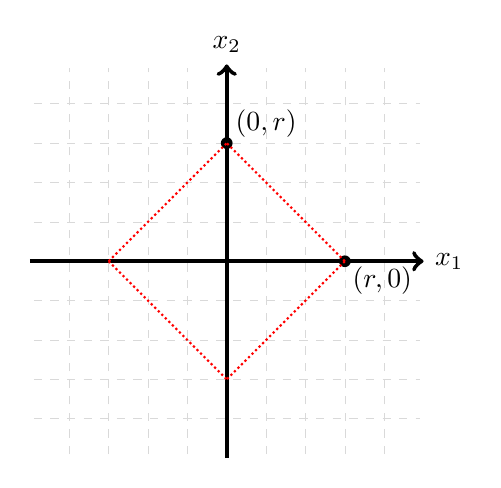
\begin{tikzpicture}[scale=0.5]
    \draw[help lines, color=gray!30, dashed] (-4.9,-4.9) grid (4.9,4.9);
    \draw[->,ultra thick] (-5,0)--(5,0) node[right]{$x_1$};
    \draw[->,ultra thick] (0,-5)--(0,5) node[above]{$x_2$};
    \node at (0,3) [circle,fill,inner sep=1.5pt]{};
    \node at (3,0) [circle,fill,inner sep=1.5pt]{};
    \node at (3.95,-0.5) {$(r,0)$};
    \node at (1,3.5) {$(0,r)$};
    
    \draw[densely dotted, thick, color=red] (3,0)--(0,3);
    \draw[densely dotted, thick, color=red] (-3,0)--(0,-3);
    \draw[densely dotted, thick, color=red] (-3,0)--(0,3);
    \draw[densely dotted, thick, color=red] (3,0)--(0,-3);
    \end{tikzpicture}}
    \subfloat[2-norm (Euclidean metric)]{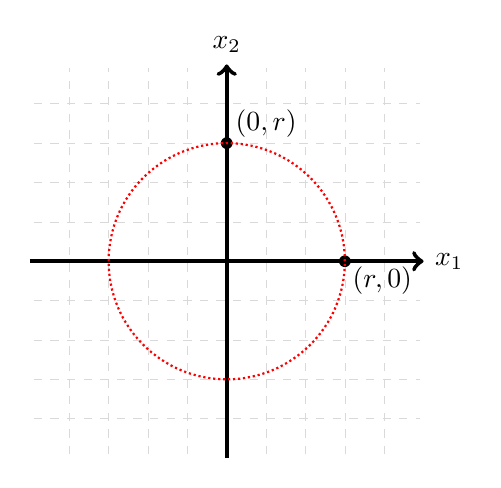
\begin{tikzpicture}[scale=0.5]
    \draw[help lines, color=gray!30, dashed] (-4.9,-4.9) grid (4.9,4.9);
    \draw[->,ultra thick] (-5,0)--(5,0) node[right]{$x_1$};
    \draw[->,ultra thick] (0,-5)--(0,5) node[above]{$x_2$};
    \node at (0,3) [circle,fill,inner sep=1.5pt]{};
    \node at (3,0) [circle,fill,inner sep=1.5pt]{};
    \node at (3.95,-0.5) {$(r,0)$};
    \node at (1,3.5) {$(0,r)$};
    
    \draw[densely dotted,thick, color = red] (0,0) circle [radius=3];
    \end{tikzpicture}}
    \subfloat[$\infty$-norm]{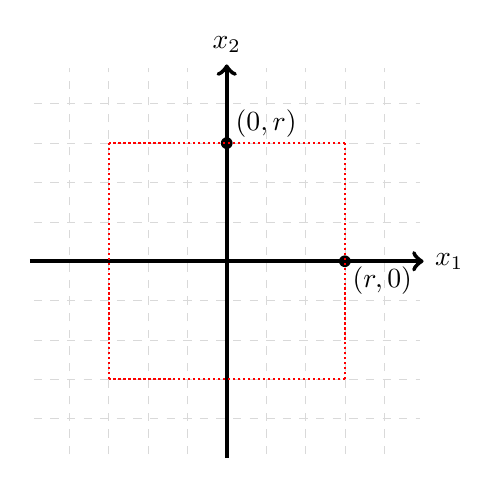
\begin{tikzpicture}[scale=0.5]
    \draw[help lines, color=gray!30, dashed] (-4.9,-4.9) grid (4.9,4.9);
    \draw[->,ultra thick] (-5,0)--(5,0) node[right]{$x_1$};
    \draw[->,ultra thick] (0,-5)--(0,5) node[above]{$x_2$};
    \node at (0,3) [circle,fill,inner sep=1.5pt]{};
    \node at (3,0) [circle,fill,inner sep=1.5pt]{};
    \node at (3.95,-0.5) {$(r,0)$};
    \node at (1,3.5) {$(0,r)$};
    
    \draw[densely dotted, thick, color=red] (3,-3) --(3,3);
    \draw[densely dotted, thick, color=red] (3,3) --(-3,3);
    \draw[densely dotted, thick, color=red] (-3,-3) --(-3,3);
    \draw[densely dotted, thick, color=red] (3,-3) --(-3,-3);
    \end{tikzpicture}}
    \caption{$B_r(0)$ for different metrics}
    \label{fig:open_ball}
\end{figure}

\end{example}

\begin{definition}[Open and closed sets]
Let $(X,d)$ be a metric space. 
\begin{itemize}
    \item A set $U \subseteq X$ is \emph{open} if for every $x \in U$ there exists $\epsilon>0$ such that $B_\epsilon(x) \subseteq U$.
    \item A set $F \subseteq X$ is \emph{closed} if $F^c:= X\setminus F$ is open.
\end{itemize}
\end{definition}

We note that $\emptyset$ and $X$ are both open and closed! 

\vspace{1em}

\begin{proposition}
\label{prop:open_sets}
Let $(X,d)$ be a metric space. 
 \begin{enumerate}
     \item[(i)] Let $A_1,A_2\subseteq X$. If $A_1$ and $A_2$ are open, then $A_1 \cap A_2$ is open.
     \item[(ii)] If $A_i \subseteq X$, $i \in I$ are open, then $\cup_{i\in I} A_i$ is open.
 \end{enumerate}
\end{proposition}
\begin{proof}
(i) Since $A_1$ is open, for each $x \in A_1$, there exists an $\epsilon_1 > 0$ such that $B_{\epsilon_1}(x) \subseteq  A_1$. Since $A_2$ is open, for each $x \in A_2$, there exists an $\epsilon_2 > 0$ such that $B_{\epsilon_2}(x) \subseteq A_2$. Let $x \in A_1 \cap A_2$. Choose $\epsilon = \min\{\epsilon_1,\epsilon_2\}$. Then  $B_{\epsilon}(x) \subseteq A_1 \cap A_2$ as required. 

(ii) Let $x\in \cup_{i\in I} A_i$. Then there exists $i \in I$ such that $x \in A_i$, and since $A_i$ is open there exists $\epsilon>0$ such that $B_\epsilon(x) \subseteq  A_i$. Since $A_i \subseteq \cup_{i\in I} A_i$, we are done.
\end{proof}

\textbf{Remark:}
These properties of open sets are used to define a topology in a more general setting. In particular, we specify a topology by specifying which sets are open.

Using DeMorgan, we immediately have the following corollary:
\begin{corollary}
\label{cor:closed_sets}
Let $(X,d)$ be a metric space. 
 \begin{enumerate}
     \item[(i)] Let $A_1,A_2\subseteq X$. If $A_1$ and $A_2$ are closed, then $A_1 \cup A_2$ is closed.
     \item[(ii)]  If $A_i \subseteq X$, $i \in I$ are closed, then $\cap_{i\in I} A_i$ is closed.
 \end{enumerate}
\end{corollary}

\begin{definition}[Interior and closure]
Let $A\subseteq X$ where $(X,d)$ is a metric space. 
\begin{itemize}
    \item The \emph{closure} of $A$ is  $\overline A :=\{x \in X: \forall \epsilon > 0 \; B_\epsilon(x) \cap A \neq \emptyset \}$
    \item The \emph{interior} of $A$ is  $\interior A :=\{x \in X: \exists \epsilon > 0 \text{ s.t. } B_\epsilon(x) \subseteq A \}$
    \item The \emph{boundary} of $A$ is $\partial A := \{ x \in X: \forall \epsilon > 0, \, B_\epsilon(x) \cap A \neq \emptyset \text{ and }  B_\epsilon(x) \cap A^c \neq \emptyset\}$
\end{itemize}
\end{definition}
The closure of a set is the smallest closed set that contains it while the interior of a set is the largest open set contained by it. 



\begin{example}
Let $X = (a, b] \subseteq \R$ with the ordinary (Euclidean) metric. Then $\overline X = [a,b]$, $\interior X = (a,b)$ and $\partial X = \{a,b\}$.
\end{example}

\begin{proposition}
 Let $A\subseteq X$ where $(X,d)$ is a metric space. Then $\interior A = A \setminus \partial A$.
\end{proposition}
\begin{proof}
First, we show $\interior A\subseteq A \setminus \partial A$. Let $x \in \interior A$. Then by definition $\exists \epsilon > 0 \text{ s.t. } B_\epsilon(x) \subseteq A$. Clearly $x \in A$ and also $\exists \epsilon > 0$ such that $B_\epsilon(x) \cap A^c = \emptyset$. Thus by definition, $x \notin \partial A$. Thus $x \in A \setminus \partial A$.

Next, we show $A \setminus \partial A \subseteq \interior A$. Let $x \in A \setminus \partial A$. Then $x \in A$ and $x \notin \partial A$. The latter means that $\exists \epsilon > 0$ such that $B_\epsilon(x) \cap A = \emptyset$ or  $B_\epsilon(x) \cap A^c = \emptyset$. Since $x \in A$, $x \in B_\epsilon(x) \cap A$ for any $\epsilon > 0$, so the former cannot be true. Therefore $\exists \epsilon > 0$ such that $B_\epsilon(x) \cap A^c = \emptyset$, i.e. $B_\epsilon(x) \subseteq A$. Thus $x \in \interior A$.
\end{proof}


\begin{proposition}
 Let $(X,d)$ be a metric space and $A\subseteq X$. $\overline A$ is closed and $\interior A$ is open.
\end{proposition}
\begin{proof}
Clearly, $\interior A$ is open by definition. We show $\overline A$ is closed by showing $(\overline A)^c$ is open. Let $x \in (\overline A)^c$. We need to show there exists $\epsilon>0$ such that $B_\epsilon(x) \subseteq (\overline A)^c$. We have that $x \notin \overline A$ so by the definition of $\overline A$, this means there exists an $\tilde \epsilon  > 0$ such that $B_{\tilde\epsilon}(x) \cap A = \emptyset$. Then any $y \in B_{\tilde\epsilon}(x)$ is in $(\overline A)^c$ by definition. Thus $B_{\tilde\epsilon}(x)  \subseteq (\overline A)^c$ and therefore $(\overline A)^c$ is open.
\end{proof}

\begin{remark}
In fact, we can show that the interior of $A$ is the largest open set contained in $A$ and the closure is the smallest closed set that contains $A$, i.e., that 
\begin{align*}
\interior A &=\bigcup \{U: U \text{ is open and } U \subseteq A \} \, , \\\overline{A} &= \bigcap \{F \colon F \text{ is closed and } A \subseteq F\} \, .
\end{align*}
This result is proved in \cref{prop:closed}.
\end{remark}

\subsection{Sequences}

\begin{definition}
Let $(X,d)$ be a metric space. A \emph{sequence} is an ordered list of points $x_n$, $n\in\N$, in $X$, denoted $(x_n)_{n \in \N}$. We say that a sequence $(x_n)_{n \in \N}$ \emph{converges} to a point $x \in X$ if 
\begin{equation*}
    \forall \epsilon > 0 \, \exists \, n_\epsilon \in \N \text{ s.t. } d(x_n,x) < \epsilon \text{ for all } n \geq n_\epsilon .
\end{equation*}
\end{definition}

\begin{proposition}
\label{prop:closure_limit}
Let $(X, d)$ be a metric space, and let $A \subseteq X$. Then $\overline A$ is equal to the set of points in $X$ which are limits of a sequence in $A$.
\end{proposition}

\begin{proof}
Let $x \in \overline A$. Then by definition, for every $\epsilon > 0$, $B_\epsilon(x) \cap A \neq \emptyset$. In particular this is true for $\epsilon = 1/n$. Thus, for any $n \in N$, we can choose an $x_n \in A$ such that $x_n \in B_{1/n}(x)$, which means $d(x,x_n) < \frac{1}{n}$ by the definition of an open ball. Since $1/n$ decreases monotonically to zero, we must have $x_n \to x$.

Let $x \in X$ be the limit of a sequence $(x_n)_{n \in \N} \in A$. Then for $\epsilon > 0$, $\exists \, n_\epsilon \in \N$ such that $d(x_n,x) < \epsilon$ for all $n \geq n_\epsilon$. This means $x_n \in B_\epsilon(x)$, and since $x_n \in A$, $B_\epsilon(x) \cap A \neq \emptyset$. Thus $x \in \overline A$.
\end{proof}

Combining this result with the fact that $A \subseteq X$ is closed if and only if $A = \overline A$ (exercise), gives the following useful way to characterize closed sets. 

\begin{corollary}
\label{cor:closed_converge}
A set $F \subseteq X$, where $(X, d)$ is a metric space, is closed if and only if every sequence in $F$ which converges in $X$ converges to a point in $F$.
\end{corollary}

We also define a concept related to the closure of a set: a cluster or accumulation point.

\begin{definition}
Let $(X,d)$ be a metric space and $A \subseteq X$. A point $x \in X$ is a \emph{cluster point} of $A$ (also called accumulation point) if for every $\epsilon >0$, $B_\epsilon(x)$ contains infinitely many points in $A$.
\end{definition}


\begin{proposition}
\label{prop:cluster_seq}
 $x \in X$ is a cluster point of $A \subseteq X$ where $(X,d)$ is a metric space if and only if there exists a sequence of points $x_n \in A$, $n \in \N$, such that $x_n \to x$.
\end{proposition}

\begin{proof}
($\Leftarrow$) Suppose there exists a sequence $(x_n)_{n \in N}$ in $A$ such that $x_n \to x$. Then for every $\epsilon >0$, by the definition of a convergent sequence, $B_\epsilon(x)$ contains infinitely many elements of the sequence $x_n$ (in particular, $\exists n_0 \in \N$ such that $x_n \in B_\epsilon(x)$ for all $n \geq n_0$). Since each $x_n \in A$, $x$ is a cluster point of $A$.

($\Rightarrow$) Suppose $x$ is a cluster point of $A$. Then for any $\epsilon > 0$, $\exists x_\epsilon \in A$ such that $x_\epsilon \in B_\epsilon(x)$. In particular, take $\epsilon = 1/n$. Then $\exists x_n \in A$ such that $x_n\in B_{1/n}(x)$. By construction, such $x_n$ form a sequence in $A$ that converges to $x$. 

\end{proof}

Combining \cref{prop:closure_limit} and \cref{prop:cluster_seq} gives the following: 

\begin{corollary}
For $A \subseteq X$, $(X,d)$ a metric space, we have $\overline{A} = A \cup \{x \in X : x \text{ is a cluster point of }A \}$.
\end{corollary}

\subsubsection{Cauchy sequences}

\begin{definition}[Cauchy sequence]
Let $(X,d)$ be a metric space. A sequence denoted $(x_n)_{n \in \N} \in X$ is called a \emph{Cauchy sequence} if
\begin{equation*}
    \forall \epsilon >0  \; \exists \, n_\epsilon \in \N \text{ s.t. } d(x_n,x_m) < \epsilon \text{ for all } n,m \geq n_\epsilon .
\end{equation*}
\end{definition}

\begin{proposition}
\label{prop:converge_means_Cauchy}
Let $(X, d)$ be a metric space, and let $(x_n)_{n\in\N}$ be a convergent sequence in $X$. Then  $(x_n)_{n\in\N}$ is Cauchy.
\end{proposition}

\begin{proof}
Let $\epsilon > 0$ be arbitrary. Let $(x_n)_{n\in\N}$ be a convergent sequence in a metric space $(X,d)$. Then there exists $n_\epsilon \in \N$ such that $d(x_n,x) < \frac{\epsilon}{2}$ for all $n \geq n_\epsilon$. Then for $n,m \geq n_\epsilon$, using the triangle inequality we have
\begin{equation*}
    d(x_n,x_m) \leq  d(x_n,x) +  d(x,x_m) < \frac{\epsilon}{2} + \frac{\epsilon}{2} = \epsilon .
\end{equation*}
Thus $(x_n)_{n\in\N}$ is Cauchy.
\end{proof}

\begin{definition}
A metric space where every Cauchy sequence converges (to a point in the space) is called \emph{complete}.
\end{definition}

In addition, a normed space that is complete with respect to the metric induced by the norm is called a \emph{Banach space}. $\R^n$ with the Euclidean distance is complete (and is, in fact, a Banach space). 
%Note that this form of completeness is slightly weaker than the completeness mentioned in \cref{ax: completeness}, however, we will not go in to detail. 

\begin{proposition}[{\cite[Proposition 2.4.5]{tastetopology}}]
\label{prop:closed_subset_complete}
Let $(X, d)$ be a metric space, and let $Y\subseteq X$.
\begin{enumerate}
    \item[(i)] If $X$ is complete and if $Y$ is closed in $X$, then $Y$ is complete.
    \item[(ii)] If $Y$ is complete, then it is closed in $X$.
\end{enumerate}
\end{proposition}

\begin{proof}
(i) Let $X$ be a complete metric space and $Y$ be a closed subset of $X$. Let $(x_n)_{n\in\N}$ be a Cauchy sequence in $Y$. Since $Y \subseteq X$, $(x_n)_{n\in\N}$ is also a Cauchy sequence in $X$. Therefore $(x_n)_{n\in\N}$ converges to an $x \in X$ since $X$ is complete. But since $Y$ is closed, by \cref{prop:closure_limit}, we must have $x \in Y$. Therefore $Y$ is complete.

(ii) Let $(X, d)$ be a metric space and let $Y\subseteq X$ be complete. Let $(y_n)_{n\in\N}$ be a sequence in $Y$ that converges to some point $y \in X$.  By \cref{prop:converge_means_Cauchy},  $(y_n)_{n\in\N}$ is Cauchy in $X$ and therefore also in $Y$. Since $Y$ is complete, $(y_n)_{n\in\N}$ converges to a point $y' \in Y$. Since sequences in metric spaces converge to unique points (see exercises), $y=y'$. Thus $Y$ is closed by \cref{cor:closed_converge}.
\end{proof}

\subsubsection{Subsequences}

\begin{definition}
Let $(x_n)_{n \in \N}$ be a sequence in a metric space $(X,d)$. Let $(n_k)_{k \in \N}$ be a sequence of natural numbers with $n_1 < n_2 < \cdots$. The sequence $(x_{n_k})_{k \in \N}$ is called a \emph{subsequence} of $(x_n)_{n \in \N}$. If $(x_{n_k})_{k \in \N}$ converges to $x \in X$, we call $x$ a \emph{subsequential limit}.
\end{definition}

\begin{example}
The sequence $\left((-1)^n\right)_{n \in \N}$ diverges but the subsequences $\left((-1)^{2n}\right)_{n \in \N}$ and $\left((-1)^{2n-1}\right)_{n\in \N}$ converge to subsequential limits 1 and $-1$, respectively.
\end{example}

\begin{proposition}
A sequence $(x_n)_{n \in \N}$ in a metric space $(X,d)$ converges to $x \in X$ if and only if every subsequence of $(x_n)_{n \in \N}$  also converges to $x$.
\end{proposition}
\begin{proof}
($\Leftarrow$) If every subsequence of $(x_n)_{n \in \N}$ converges to $x \in X$, then  $(x_n)_{n \in \N}$ must converge to it as well, since a sequence is a subsequence of itself. 

($\Rightarrow$) Suppose $(x_n)_{n \in \N}$ converges to $x \in X$ and let $(x_{n_k})_{k \in \N}$ be an arbitrary subsequence of $(x_n)_{n \in \N}$. Let $\epsilon > 0$ be arbitrary. There exists $n_\epsilon \in \N$ such that $d(x_n,x) < \epsilon$ for all $n \geq n_\epsilon$. Choose $k_\epsilon$ such that $n_{k_\epsilon} \geq n_\epsilon$, which must exist since $(n_k)_{k\in\N}$ is strictly increasing. Then for all $k \geq k_\epsilon$, $d(x_{n_k},x) < \epsilon$. Thus $(x_{n_k})_{k \in \N}$ converges to $x$.
\end{proof}


\subsection{Continuity}

\begin{definition}
Let $(X,d_X)$ and $(Y,d_Y)$ be metric spaces, let $x_0 \in X$, and let $f:X\to Y$. $f$ is \emph{continuous} at $x_0$ if for every sequence $(x_n)_{n\in\N}$ in $X$ that converges to $x_0$, we have $\lim_{n\to\infty}f(x_n)=f(x_0)$.
We say that $f$ is \emph{continuous} if it is continuous at every point in $X$.
\end{definition}

\begin{theorem}[{\cite[Theorem 2.3.7.]{tastetopology}}]
\label{thm:cont_equiv}
Let $(X,d_X)$ and $(Y,d_Y)$ be metric spaces, let $x_0 \in X$, and let $f:X\to Y$. The following are equivalent:
\begin{enumerate}
    \item[(i)] $f$ is continuous at $x_0$
    \item[(ii)] for all $\epsilon>0$, there exists $\delta > 0$ such that $d_Y(f(x),f(x_0))) < \epsilon$ for all $x \in X$ with $d_X(x,x_0) < \delta$
    \item[(iii)] for each $\epsilon>0$, there is $\delta > 0$ such that $B_\delta(x_0) \subseteq f^\inv (B_\epsilon(f(x_0)))$
\end{enumerate}
\end{theorem}

\begin{proof}
(i) $\Rightarrow$ (ii) We prove the contrapositive. Assume
\begin{equation}
\label{star1} 
\exists \epsilon_0 \text{ such that } \forall \delta > 0 \text{ there exists an } x_\delta \in X \text{ with } d_X(x_\delta,x_0) < \delta \text{ and } d_Y(f(x_\delta),f(x_0))) \geq \epsilon_0
\tag{$\star$}
\end{equation}
We need to find a sequence in $X$ that converges to  $x_0$ but the sequence of images does not converge. Let's construct such a sequence. 

Let $\delta=\frac{1}{n}$ in \eqref{star1} for $n \in \N$. Then we can pick a sequence $x_n := x_{1/n}$ given by \eqref{star1} which converges to $x_0$. However, for each $n \in \N$, we have $d_Y(f(x_n),f(x_0))) \geq \epsilon_0$, so we cannot have $\lim_{n\to\infty}f(x_n)=f(x_0)$.

(ii) $\Rightarrow$ (iii) Follows from the definitions of the pre-image and open balls. 

(iii) $\Rightarrow$ (i) Let $(x_n)_{n\in\N}$ be a sequence in $X$ that converges to $x_0$. Let $\epsilon > 0$. Then by (iii), there exists $\delta > 0$ such that $B_\delta(x_0) \subseteq f^\inv (B_\epsilon(f(x_0)))$, i.e. if $x$ is such that $d_X(x,x_0) < \delta$, then $x$ is such that  $d_Y(f(x),f(x_0)) < \epsilon$. By the definition of convergence, there exists an $N \in \N$ such that $d(x_n,x_0)< \delta$ for all $n \geq N$. Then by (iii), $d(f(x_n),f(x_0))< \epsilon$ for all $n \geq N$. Thus $\lim_{n\to\infty}f(x_n)=f(x_0)$.
\end{proof}

\begin{corollary}
\label{cor:open_closed}
Let $(X,d_X)$ and $(Y,d_Y)$ be metric spaces and let $f:X\to Y$. The following are equivalent:
\begin{enumerate}
    \item[(i)] $f$ is continuous
    \item[(ii)] if $U \subseteq Y$ is open, then $f^\inv(U)$ is open
    \item[(iii)] if $F \subseteq Y$ is closed, then $f^\inv(F)$ is closed
\end{enumerate}
\end{corollary}

\textit{Note: the following proof uses the following results, which you may wish to prove as an exercise using techniques from the set theory section if they are not clear to you: Let $X$ and $Y$ be sets and $f:X \to Y$. Let $A,B \subseteq Y$. Then 
\begin{enumerate}
\item $A \subseteq B$ $\implies$ $f^\inv(A) \subseteq f^\inv(B)$
\item $f^\inv(Y \setminus A) = X \setminus f^\inv(A)$
\end{enumerate}}

\begin{proof}
Let $(X,d_X)$ and $(Y,d_Y)$ be metric spaces and let $f:X\to Y$.

(i) $\Rightarrow$ (ii): Suppose $f$ is continuous (on every point in $X$) and let $U \subseteq Y$ be open. Let $x \in f^\inv(U)$, then $f(x) \in U$, and since $U$ is open, there exists $\epsilon_0 > 0$ such that $B_{\epsilon_0}(f(x)) \subseteq U$. By \cref{thm:cont_equiv}(iii), there exists a $\delta_0 > 0$ such that $B_{\delta_0}(x) \subseteq f^\inv (B_{\epsilon_0}(f(x)))$. Since $B_{\epsilon_0}(f(x))) \subseteq U$, $f^\inv (B_{\epsilon_0}(f(x))) \subseteq f^\inv(U)$. Thus for each $x \in f^\inv(U)$, there exists $\delta_0$ such that $B_{\delta_0}(x) \subseteq f^\inv (B_{\epsilon_0}(f(x))) \subseteq f^\inv(U)$, so $f^\inv(U)$ is open.

(ii) $\Rightarrow$ (i): We want to prove that $f$ is continuous at every $x \in X$ using the definition from \cref{thm:cont_equiv}(iii), i.e. we must show that for $x \in X$, for each $\epsilon>0$, there is $\delta > 0$ such that $B_\delta(x) \subseteq f^\inv (B_\epsilon(f(x)))$. 

Let $x\in X$ and let $\epsilon > 0$ be arbitrary. Since $B_\epsilon(f(x))$ is an open set, by (ii), $f^\inv(B_\epsilon(f(x)))$ is also open. Since $x \in f^\inv(B_\epsilon(f(x)))$, there exists a $\delta > 0$ such that $B_\delta(x) \subseteq f^\inv(B_\epsilon(f(x)))$ by the definition of a set being open, so we are done.

(ii) $\Rightarrow$ (iii): Let $F \subseteq Y$ be closed. Then $Y \setminus F$ is open, so by (ii), $f^\inv(Y \setminus F)$ is open as well. Since $f^\inv(Y \setminus F) = X\setminus f^\inv(F)$, $f^\inv(F)$ is closed.

(iii) $\Rightarrow$ (ii) follows from the above, exchanging ``open'' and ``closed''.
\end{proof}


\begin{definition}
\label{def:Lip_unif}
Let $(X,d_X)$ and $(Y,d_Y)$ be metric spaces and let $f:X\to Y$. 
\begin{itemize}
    \item $f$ is \emph{uniformly continuous} if for all $\epsilon>0$, there exists $\delta > 0$ such that for every $x_1,x_2\in X$ with $d_X(x_1,x_2) < \delta$, we have  $d_Y(f(x_1),f(x_2))) < \epsilon$ 
    \item $f$ is \emph{Lipschitz continuous} if there exists a $K > 0$ such that for every $x_1,x_2\in X$ we have  $d_Y(f(x_1),f(x_2))) \leq K d_X(x_1,x_2)$
\end{itemize}
\end{definition}

\begin{proposition}
Let $(X,d_X)$ and $(Y,d_Y)$ be metric spaces and let $f:X\to Y$. 
$$f \text{ is Lipschitz continuous } \Rightarrow \text{ f is uniformly continuous } \Rightarrow \text{ f is continuous}$$
\end{proposition}

The proof is left as an exercise. 

\begin{definition}
Let $(X,d)$ be a metric space and let $f:X \to X$. We say that $x^* \in X$ is a \emph{fixed point} of $f$ if $f(x^*) = x^*$.
\end{definition}

\begin{definition}
Let $(X,d)$ be a metric space and let $f:X \to X$. $f$ is a \emph{contraction} if there exists a constant $k \in [0,1)$ such that for all $x,y \in X$, $d(f(x),f(y))) \leq k d(x,y)$.
\end{definition}

Observe that a function is a contraction if and only if it is Lipschitz continuous with constant $K < 1$.

\begin{theorem}
Suppose that $f : X \to X$ is a contraction and the metric space $X$ is complete. Then $f$ has a unique fixed point $x^*$.
\end{theorem}

We omit the proof here; see \cite[p.240]{realanalysis} for the proof as well as more details on how to find the fixed point.

\begin{example}
Let $f:\left[-\frac{1}{3},\frac{1}{3}\right] \to \left[-\frac{1}{3},\frac{1}{3}\right]$ be defined by the mapping $x \mapsto x^2$. Assume we use the standard Euclidean metric, $d(x,y) = |x-y|$. $f$ has a unique fixed point because $\left[-\frac{1}{3},\frac{1}{3}\right]$ is a complete metric space (see \cref{prop:closed_subset_complete}) and $f$ is a contraction with Lipschitz constant 2/3.

To see that it is a contraction, let $x,y \in \left[-\frac{1}{3},\frac{1}{3}\right]$. Then
\begin{equation*}
   |x^2 - y^2| = |x+y| |x-y| \leq \tfrac{2}{3} |x-y|. 
\end{equation*}
\end{example}


\subsection{Equivalence of metrics}

\begin{definition}[Equivalent metrics]
Two metrics $d_1$ and $d_2$ on a set $X$ are \emph{equivalent} if the identity maps from $(X,d_1)$ to $(X,d_2)$ and from $(X,d_2)$ to $(X,d_1)$ are continuous. 
\end{definition}

The following result follows from the definition and \cref{cor:open_closed}:

\begin{proposition}
Two metrics $d_1$, $d_2$ on a set $X$ are equivalent if and only if they have the same open sets or the same closed sets.
\end{proposition}

So, in a certain sense, equivalent metrics induce the same structure.

\begin{definition}
Two metrics $d_1$ and $d_2$ on a set $X$ are \emph{strongly equivalent} if for every $x,y\in X$, there exists constants $\alpha>0$ and $\beta>0$ such
\begin{equation*}
    \alpha d_1(x,y) \leq d_2(x,y) \leq \beta d_1(x,y).
\end{equation*}
\end{definition}

If two metrics are strongly equivalent then they are equivalent. The proof of this is part of the exercises. 

\begin{example}
We show that the Euclidean distance (induced by 2-norm) and the metric induced by the $\infty$-norm are equivalent on $\R^n$. 

\vspace{1em}
Let $\|x-y\|_2=\sqrt{\sum_{j=1}^n (x_j - y_j)^2}$ be the Euclidean metric and $\|x-y\|_\infty= \max_{j=1,\ldots,n} |x_j - y_j|$ be the metric induced by the $\infty$-norm. We have
\begin{equation*}
   \|x-y\|_2 = \sqrt{\sum_{j=1}^n (x_j - y_j)^2} \leq  \sqrt{ n \max_{j=1,\ldots,n} (x_j - y_j)^2}  = \sqrt{n} \max_{j=1,\ldots,n} |x_j - y_j| = \sqrt{n} \, \|x-y\|_\infty
\end{equation*}
and
\begin{equation*}
    \|x-y\|_\infty = \max_{j=1,\ldots,n} |x_j - y_j|  = \sqrt{\max_{j=1,\ldots,n} (x_j - y_j)^2} \leq \sqrt{\sum_{j=1}^n(x_j - y_j)^2}  = \|x-y\|_2  \, .
\end{equation*}
Thus the two metrics are strongly equivalent. 
\end{example}

\subsection{Density and separability}

The content in the next two sections (density, separability, and compactness) is covered in more generality in \cref{app:topology}. Please see that section for these topics and more on a general topological space.

We first consider the concept of density in metric spaces. 

\begin{definition}
Let $(X,d)$ be a metric space. A subset $A\subseteq X$ is called \emph{dense} if $\overline{A} = X$.
\end{definition}

Using the definition of closure, we see that $A\subseteq X$ is dense if and only if for all $x\in X$ and $\varepsilon>0$, $B_\varepsilon(x)\cap A \neq \emptyset$.


\begin{example}
\textcolor{white}{Skip}
\begin{itemize}
    \item The rationals $\Q$ are dense in the reals $(\R,\vert \cdot \vert)$.
    \item Let $X$ be a set and define $d\colon X \times X \to \mathbb{R}$ by 
    \begin{align*}
        d(x,y) = \begin{cases}
            0, & \; x=y, \\
            1, & \; x\neq y.
        \end{cases}
    \end{align*}
    This is a metric (see \cref{exercises:metric_spaces}, Exercise 3). The only dense set in this metric space is $X$ itself. 
\end{itemize}
\end{example}

The concept of a dense subset allows us in a way to look at that set instead of the whole space. In the metric space setting, this means that elements in $X$ can be approximated arbitrarily well with elements from the dense subset.

\begin{definition}
A metric space $(X,d)$ is \emph{separable} if it contains a countable dense subset.
\end{definition}

As stated in the previous example, $\Q$ is dense in $\R$, and since $\Q$ is countable, $\R$ is separable. We could extend this example to $\R^n$. However, if we look at all bounded real-valued sequences with the metric induced by the supremum norm, this space fails to be separable. 

\begin{example}
Define $\ell_\infty=\{ (x_n)_{n\in \N} \, : x_n \in \R , \; \sup_{n\in \N} \vert x_n \vert <\infty \}$, the space of bounded real valued sequences. We can endow $\ell_\infty$ with a metric induced by the supremum norm, namely $d((x_n)_{n\in \N}, (y_n)_{n\in \N}) = \sup_{n\in \N} \vert x_n-y_n\vert$. 
Then $\ell_\infty$ is not separable with respect to the topology induced by this metric. 

To see this, for each $M\subseteq \N$ define 
\begin{equation*}
    e^M_n = \begin{cases} 1 \; \text{ if } n \in M,\\
    0 \; \text{ otherwise},
    \end{cases}
\end{equation*}
for $n \in \N$. 

Then if $M_1, M_2\subseteq \N$ are non-empty with $M_1\neq M_2$, $d((e^{M_1}_n)_{n\in \N},(e^{M_2}_n)_{n\in \N}) = 1$. Thus the open balls $B_{1/3}((e^{M_1}_n)_{n \in \N})$, $B_{1/3}((e^{M_2}_n)_{n \in \N})$ are disjoint for all non-empty $M_1, M_2\subseteq \N$ with $M_1\neq M_2$ (check using contradiction and triangle inequality).

Now suppose towards contradiction that there exists $A \subseteq \ell^\infty$ that is dense and countable.  Then by density, for all $(x_n)_{n \in \N} \in \ell_\infty$ and for all $\varepsilon>0$, $B_\varepsilon((x_n)_{n \in \N})\cap A \neq \emptyset$. In particular for all $M \subseteq \N$, $B_{1/3}((e^{M}_n)_{n \in \N})\cap A \neq \emptyset$. 

However, there are uncountably many such $M$ because $\cP(\N)$ is uncountable (see \cref{thm:cantor}), but only countably many elements in $A$. Since the balls are disjoint, this is a contradiction. 
\end{example}

\subsection{Compactness}

Next, we discuss the idea of compactness on a metric space. This idea generalizes the concept of a closed and bounded set in Euclidean space to a general metric space. It can be further generalized to any topological space. 

\begin{definition}[Compact]
Let $(X,d)$ be a metric space and let $K\subseteq X$. A collection $\{U_i\}_{i\in I} $ of open sets is called \emph{open cover} of $K$ if $K\subseteq \cup_{i\in I} U_i$. The set $K$ is called \emph{compact} if for all open covers $\{U_i\}_{i\in I}$ there exists a finite subcover, meaning there exists an $n\in \N$ and $\{U_1,\ldots,U_n\}\subseteq \{U_i\}_{i\in I}$ such that $K\subseteq \cup_{i=1}^n U_i$.
\end{definition}

The next example explains the connection to finite sets

\begin{example}
Let $S\subseteq X$ where $(X,d)$ is a metric space. If $S$ is finite, then it is compact. 
\end{example}
\begin{proof}
Since $S$ is finite, we can write $S = \{ x_1, \ldots, x_n\}$. For any open cover $\mathcal{U} = \{ U_i \}_{i\in I}$, for $j=1,\ldots,n$ there exists $U_j \in \mathcal{U}$ such that $x_j \in U_j$. Thus $S \subseteq \cup_{j=1}^n U_j$, so $S$ is compact.
\end{proof}

\begin{example}
$(0,1)$ is not compact.
\end{example}
\begin{proof}
The set $\{U_n\}_{n \in N}$ where $U_n = \left(\frac{1}{n},1\right)$ is an open cover for $(0,1)$ since $(0,1) \subseteq \cup_{n=1}^\infty \left(\frac{1}{n},1\right)$. Suppose in order to derive a contradiction that there exists a finite subcover, i.e. there exists $N \in \N$ such that $(0,1) \subseteq \cup_{j=1}^N \left(\frac{1}{n_j},1\right)$. Since $\left(\frac{1}{n},1\right) \subseteq \left(\frac{1}{m},1\right)$ for $m \geq n$ (the sets are nested), this means $(0,1) \subseteq  \left(\frac{1}{n_N},1\right)$. But clearly there exists an $x \in (0,1)$ such that $0 < x < \frac{1}{n_N}$ for any finite $n_N$. Contradiction. Therefore $(0,1)$ is not compact.
\end{proof}

In fact, the next proposition shows that compactness implies that a set is closed.

\begin{proposition}[{\cite[Proposition 3.3.6]{tastetopology}}]Let $(X,d)$ be a metric space and take a non-empty subset $K\subseteq X$. The following holds:
\begin{enumerate}
    \item If $X$ is compact and $K$ is closed, then $K$ is compact (i.e. closed subsets of compact sets are compact).
    \item If $K$ is compact, then $K$ is closed.
\end{enumerate}
\end{proposition}
\begin{proof}
1. We need to show that any open cover of $K$ has a finite subcover. Let $\{U_i\}_{i\in I}$ be an open cover of $K$. Then, since $K^c$ is open, $\{U_i\}_{i\in I} \cup {K^c}$ is an open cover of $X$. Since $X$ is compact there exists a finite subcover. There are two possibilities,  the finite subcover is either of the form $\{U_1, \ldots, U_n, K^c\}$ or $\{U_1, \ldots, U_n\}$. In either case, $\{U_1, \ldots, U_n\}$ is a finite subcover for $K$ since $K \subseteq X$. Hence, $K$ is compact. 
    
2. We will show that $K^c$ is open. We do this by showing that for each $x\in K^c$, there exists an open ball in $K^c$ that contains $x$.

Let $x\in K^c$. By the properties of the metric for all $y\in K$, $d(x,y)>0$. Thus, $B_\frac{d(x,y)}{2}(y)$ and $B_\frac{d(x,y)}{2}(x)$ are disjoint.  Since $K$ is compact and $\{B_\frac{d(x,y)}{2}(y)\}_{y\in K}$ is an open cover of $K$, there exist $y_1,\ldots, y_n$ such that $K\subseteq \cup_{i=1}^n B_\frac{d(x,y)_i}{2}(y_i)$.

Then $U_x := \cap_{i=1}^n B_\frac{d(x,y_i)}{2}(x)$ is an open set by \cref{prop:open_sets} that contains $x$ by definition, and it is a subset of $K^c$ since each set in the intersection is disjoint from a set that forms the open cover for $K$. Since $U_x$ is open and $x\in U_x$, there exists $\varepsilon>0$ such that $B_\varepsilon(x) \subseteq U_x\subseteq K^c$, which shows that $K^c$ is open. Hence, $K$ is closed.
% We would like to take the intersection over the $U_{x,y}$ for $y \in K$ to obtain an open set containing $x$ and contained in $K^c$, but since the intersection is arbitrary we cannot guarantee that the resulting set is open (note that the union would not work since we want to guarantee that the resulting set is still contained in $K^c$). However, since $K$ is compact and $\{U_y\}_{y\in K}$ is an open cover of $K$ there exist $y_1,\ldots, y_n$ such that $K\subseteq \cup_{i=1}^n U_{y_i}$. Thus $\tilde U_x = \cap_{i=1}^n U_{x,y_i}$ is open and $x\in \tilde U_x$ with $\tilde U_x \subseteq K^c$. 
% This construction works for any $x\in K^c$. Thus for every $x \in K^c$, there exists a $U_x$ with $x\in \tilde U_x$. Also every $U_x$ 
% In particular, we have $K^c = \cup_{x\in K^c} \tilde U_x$. Thus, $K^c$ is open. 
\end{proof}

Just as we had a sequential characterization of the closure of a set, we similarly have a sequential characterization of compactness. 

\begin{theorem}
Let $(X,d)$ be a metric space. Then $K\subseteq X$ is compact with respect to the metric induced by $d$ if and only if every sequence in $K$ admits a subsequence converging to some point in $K$.
\end{theorem}

The proof is omitted. See \cite[Theorem 2.5.10]{tastetopology}. In undergraduate math classes you may have seen another equivalent definition for compactness on $\R^n$. This is a nice feature of Euclidean space.

\begin{theorem}[Heine-Borel theorem]
Let $K\subseteq \R^n$. Then $K$ is compact with respect to the topology induced by the Euclidean distance if and only if it is closed and bounded.
\end{theorem}

The proof is again omitted. See \cite[Corollary 2.5.12]{tastetopology}. A corollary of the Heine-Borel theorem together with the sequential characterization of compactness is the Bolzano-Weierstrass theorem.

\begin{corollary}[Bolzano-Weierstrass]
Any bounded sequence in $\R^n$ has a convergent subsequence.
\end{corollary}

Arbitrary compact metric spaces have some nice properties in general as the next proposition shows.

\begin{proposition}
    A compact metric space $(X,d)$ is complete and separable.
\end{proposition}

The proof of this statement can be found in \cite[Proposition 2.5.8]{tastetopology}. We will end this section by highlighting the connection between continuous functions and compactness. The next proposition is, in a certain sense, a generalization of the extreme value theorem to arbitrary metric spaces.

\begin{proposition}
Let $(X,d_X)$ and $(Y, d_Y)$ be metric spaces. Suppose $K\subseteq X$ is compact and let $f\colon K \to Y$ be continuous. Then $f(K)$ is compact. 
\end{proposition}

\begin{proof}
We will use the characterization of continuity given in \cref{cor:open_closed}. Let $\{U_i\}_{i\in I}$ be an open cover of $f(K)$, i.e. $f(K) \subseteq \bigcup_{i\in I} U_i$. Then $f^{-1}(f(K)) \subseteq f^{-1}(\bigcup_{i\in I} U_i)$. 

By Exercise 9 in \cref{subsec:ex_set_theory}, we have $f^{-1}(\bigcup_{i\in I} U_i) = \bigcup_{i\in I}f^{-1} (U_i)$ and by \cref{prop:set_subset_preim_im}, we have $K\subseteq f^{-1}(f(K))$. Hence, we obtain $K \subseteq \bigcup_{i\in I}f^{-1} (U_i)$. 

Since $f$ is continuous, each $f^{-1} (U_i)$ is open and thus $\{f^{-1} (U_i)\}_{i\in I}$ is an open cover of $K$. Since $K$ is compact, there exist $f^{-1}(U_1),\ldots, f^{-1}(U_n)$ such that $K \subseteq \bigcup_{i=1}^n f^{-1}(U_i)$. 

Then $f(K) \subseteq f(\bigcup_{i=1}^n f^{-1}(U_i)) = \bigcup_{i=1}^n f(f^{-1}(U_i)) \subseteq \bigcup_{i=1}^n U_i$, where we use that images preserve set inclusions (check!), and Exercises 8 and 9 in \cref{subsec:ex_set_theory}. Thus, $\{U_1,\ldots, U_n\}$ is a finite subcover for $f(K)$ and $f(K)$ is compact. 
\end{proof}

Note: this is a generalization of the Extreme Value Theorem to metric spaces.

\subsection{Extra properties of \texorpdfstring{$\R$}{R}}

Using the definition of continuity in terms of $\epsilon$-balls and equipping $\R$ with the metric induced by the absolute value, i.e. $d(x,y) = \vert x- y\vert$ for $x,y\in \R$, we obtain the usual $\epsilon-\delta$ definition of continuity. Hence, a function $f\colon \R \to \R$ is continuous at $x_0\in \R$ if for all $\epsilon>0$ there exists a $\delta>0$ such that $\vert x_0-y\vert <\delta$ implies $\vert f(x_0)-f(y)\vert<\epsilon$. Since $\R$ is also totally ordered we can also talk about left and right continuity, by separating $B_\epsilon(x) = (x-\epsilon, x+ \epsilon) = (x-\epsilon, x] \cup [x, x+\epsilon)$.

\begin{definition} Let $f\colon \R \to \R$.
\begin{itemize}
    \item $f$ is \emph{left continuous} at $x_0\in \R$ if for all $\epsilon >0$ there exists a $\delta>0$, such $\vert f(x_0)-f(x)\vert<\epsilon$ whenever $ x_0-\delta <x<x_0$.
    \item $f$ is \emph{right continuous} at $x_0\in \R$ if for all $\epsilon >0$ there exists a $\delta>0$, such $\vert f(x_0)-f(x)\vert<\epsilon$ whenever $x_0<x<x_0+\delta$.
\end{itemize}
We say that $f$ is left continuous if it is left continuous at all points in the domain, and similar for right continuous.
\end{definition}

Similar to the ordinary sense of continuity, one can describe left and right continuity in terms of sequences. 

\begin{proposition}
 A function $f\colon \R \to \R$ is continuous if and only if it is left and right continuous. 
\end{proposition}

\begin{proof}
($\Leftarrow$) Suppose $f:\R \to \R$ is both right and left continuous. Let $\epsilon > 0$ be arbitrary. Then by the definition of left continuous, there exists a $\delta_1>0$, such $\vert f(x_0)-f(x)\vert<\epsilon$ whenever $ x_0-\delta_1 <x<x_0$, and by the definition of right continuous, there exists a $\delta_2>0$, such $\vert f(x_0)-f(x)\vert<\epsilon$ whenever $x_0<x<x_0+\delta_2$.

Let $\delta = \min\{\delta_1,\delta_2\}$. Let $x \in \R$ such that $\vert x_0-x\vert <\delta$. Then $x_0- \delta < x < x_0 + \delta$. 

Case 1: Suppose $x < x_0$. Then $x_0- \delta_1 < x <x_0$, so $\vert f(x_0)-f(x)\vert<\epsilon$, so $f$ is continuous.

Case 2: Suppose $x > x_0$. Then $x_0 < x < x_0 + \delta_2$, so $\vert f(x_0)-f(x)\vert<\epsilon$, so $f$ is continuous.

If $x=x_0$, the result is trivial, so we conclude that $f$ is continuous.

($\Rightarrow$) Let $f:\R \to \R$ be continuous. Then for every $\epsilon >0$, $\exists \delta_0 > 0$ such that when $x$ is such that $|x - x_0| < \delta$, then $|f(x) - f(x_0)| < \epsilon$.

For $\epsilon > 0$ arbitrary, take $\delta_0$ from the definition of $f$ being continuous.  Take $x \in \R$ such that $x_0 < x < x_0 + \delta_0 $. Then $x_0 - \delta_0 < x < x_0 + \delta_0 $, which implies $|x - x_0| < \delta_0 $. Thus  $|f(x) - f(x_0)| < \epsilon$, so $f$ is right-continuous.

The proof for left-continuity is similar. 
\end{proof}

Using the least upper bound property of sets, we can introduce the concepts of limit inferior and limit superior as the limit of infima and suprema when we view the sequence as a set. First, we recall what it means for a sequence to be bounded.

\begin{definition}
Let $(x_n)_{n\in \N}$ be a sequence in $\R$. We call $(x_n)_{n\in \N}$ \emph{bounded} if there exists an $M > 0$ such that $\vert x_n\vert<M$ for all $n\in \N$.
\end{definition}

This definition is equivalent to the set of sequence elements being bounded in the metric space setting. Similarly, one can talk about a sequence being bounded above or below in the order theoretic setting (see \cref{sec:ordered_sets}), by looking at the set of sequence elements. The next theorem is useful.

\begin{theorem}[Monotone convergence theorem]
\label{thm:mon_conv}
\textcolor{white}{skip}
\begin{itemize}
\item[(i)] Suppose $(x_n)_{n\in \N}$ is a monotonically increasing sequence, i.e. $x_n\leq x_{n+1}$ for all $n\in \N$, and that it is bounded (above). Then the sequence converges. Furthermore, $\lim_{n\to \infty} x_n = \sup_{n\in \N} x_n$, where $\sup_{n\in \N} x_n := \sup\{x_n \; \colon \; n\in \N\}$.
\item[(ii)] Suppose $(x_n)_{n\in \N}$ is a monotonically decreasing sequence, i.e. $x_n\geq x_{n+1}$ for all $n\in \N$, which is bounded (below). Then the sequence converges and $\lim_{n\to \infty} x_n = \inf_{n\in \N} x_n := \inf\{x_n \; \colon \; n\in \N\}$. 
\end{itemize}
\end{theorem}

The proof is omitted. We call increasing or decreasing sequences monotone, hence the theorem name.

If the sequence is increasing but not bounded above, then $\lim_{n\to \infty} x_n = \infty$, and if it is decreasing but not bounded below, then $\lim_{n\to \infty} x_n = -\infty$.

 We would like to use the monotone convergence theorem for arbitrary sequences. We do so by building an increasing sequence (or decreasing) sequence from an arbitrary one. First, we recall some facts about infima and suprema and introduce the convention that $\sup A = \infty$ if $A\subseteq \R$ is not bounded above and $\inf A= -\infty$ if $A$ is not bounded below.

\begin{lemma}\label{lem:inf_sup_inequality}
If $A \subseteq B \subseteq \R$ is non-empty, then $\inf A \leq \sup A$, $\sup A \leq \sup B$, and $\inf A \geq \inf B$.
\end{lemma}
The proof of this follows from the definition of greatest lower and least upper bound. 

\begin{definition}
Let $(x_n)_{n\in \N}$ be a sequence in $\R$. We define the \emph{limit superior} of $(x_n)_{n\in \N}$ as 
$$\limsup_{n\to \infty} x_n: = \lim_{n\to \infty} \sup_{k\geq n} x_k.$$ 
Similarly we define  the \emph{limit inferior} of $(x_n)_{n\in \N}$ as 
$$\liminf_{n\to \infty} x_n: = \lim_{n\to \infty} \inf_{k\geq n} x_k.$$
\end{definition}

\begin{proposition}\label{prop:limsup_monotonicity}
Let $(x_n)_{n \in \N}$ be a sequence in $\R$.
\begin{itemize} 
\item The sequence of suprema, $s_n = \sup_{k\geq n} x_k$, is decreasing and the sequence of infima, $i_n = \inf_{k\geq n} x_k$, is increasing.
\item The limit superior and the limit inferior of a bounded sequence always exist and are finite.
\end{itemize}
\end{proposition}
\begin{proof}
The first part is true by Lemma 3.45. The second bullet point follows by the Monotone Convergence Theorem.
\end{proof}

Conceptually, we can think of the limit superior as the greatest cluster point of a sequence, and of the limit inferior as the least.
If the sequence $(x_n)_{n\in \N}$ is not bounded above, then $\limsup_{n\to \infty} x_n = \infty$. Similarly, if the sequence $(x_n)_{n\in \N}$ is not bounded below, then $\liminf_{n\to \infty} x_n = -\infty$. This is in line with our convention that $\sup A = \infty$, if $A$ is not bounded above and $\inf A = -\infty$, if $A$ not bounded below. 

\begin{theorem}
Let $(x_n)_{n\in \N}$ be a sequence in $\R$. Then the sequence converges to $x\in \R$ if and only if $\limsup_{n\to \infty} x_n= x =\liminf_{n\to \infty} x_n$.
\end{theorem}

\begin{proof}
For convenience, denote $i_n := \inf_{k\geq n} x_k$ and $s_n :=  \sup_{k\geq n} x_k$ for $n\in \N$.


($\Rightarrow$) Suppose $\lim_{n\to \infty} x_n = x\in \R$ and let $\epsilon>0$. Since the sequence converges, there exists an $N\in \N$ such that $\vert x-x_n\vert <\epsilon$, i.e. $x-\epsilon<x_n<x+\epsilon$, for all $n\geq N$. 

In particular, $x-\epsilon<x_n$ for all $n\geq N$, so $x-\epsilon$ is a lower bound for the set $\{x_n \colon n\geq N\}$. Therefore $x-\epsilon\leq i_N$. 

Similarly, since $x_n<x - \epsilon$ for all $n\geq N$, $x+\epsilon$ is an upper bound for the set $\{x_n \colon n\geq N\}$. Therefore $s_N \leq x + \epsilon$. 

By \cref{prop:limsup_monotonicity} the sequence of infima is increasing and by the Monotone Convergence Theorem, its limit is given by the supremum of the sequence. Hence, we obtain 
$$x-\epsilon\leq i_N \leq \lim_{n \to \infty} i_n =  \liminf_{n\to \infty} x_n.$$ 

Similarly, since the sequence of suprema is decreasing and using the Monotone Convergence theorem again, we obtain 
$$\limsup_{n\to \infty} x_n\leq s_N<x+\epsilon.$$
Now observe that $\liminf_{n\to \infty} x_n\leq \limsup_{n\to \infty} x_n $, since $i_n\leq s_n$ for all $n\in \N$ by \cref{lem:inf_sup_inequality} (exercise: $x_n \leq y_n$ for all $n \in \N$ implies $\lim_{n\to \infty} x_n \leq \lim_{n\to \infty} y_n$). Thus we have
\begin{align*}
    x-\epsilon \leq \liminf_{n\to \infty}x_n \leq \limsup_{n\to \infty} x_n \leq x+\epsilon.
\end{align*}
Since this holds for any $\epsilon$, the desired result follows.

($\Leftarrow$) Now suppose $\limsup_{n\to \infty} x_n= x =\liminf_{n\to \infty} x_n$. We need to show that $\lim_{n\to\infty} x_n = x$. 

Let $\epsilon>0$. Then since $\limsup_{n\to \infty} x_n = \lim_{n\to \infty} s_n= x$, there exists an $N_1\in \N$ such that $\vert s_n - x\vert <\epsilon$ for all $n\geq N_1$. In particular, 
$$x_k \leq s_{N_1} < x+\epsilon \qquad \text{ for all } k\geq N_1.$$ 

Similarly, there exists $N_2\in \N$ such that $\vert i_n - x\vert <\epsilon$ for all $n\geq N_2$ giving 
$$x-\epsilon< i_{N_2} \leq x_k  \qquad \text{ for all } k\geq N_2.$$ Hence, by setting $N= \max\{N_1,N_2\}$ we see $x-\epsilon < x_k < x+ \epsilon$ or equivalently $\vert x_k - x\vert < \epsilon$ for all $k\geq N$, which proves the result. 
\end{proof}

Note that we only talked about limit superior and limit inferior for real sequences. However, we can extend this easily to a sequence of functions $f_n \colon X \to \R$ by setting $f = \limsup_{n\to \infty } f_n$ to be the function defined pointwise by $f(x) = \limsup_{n\to \infty } (f_n (x)) $ and similar for the limit inferior. There also exists a set theoretic version in terms of unions and intersections which you will encounter in probability.

\subsection{Exercises}
\label{exercises:metric_spaces}
\begin{enumerate}
    \item Show that the infinity norm $||x||_\infty$, $x \in \R^n$, defined in \cref{p-norm} is a norm.
    \item Let $(X,d)$ be any metric space, and define $\tilde d: X \times X \to \R$ by 
    \begin{equation*}
        \tilde d(x,y) = \frac{d(x,y)}{1+d(x,y)}, \quad x,y \in X .
    \end{equation*}
    Show that $\tilde d$ is a metric on $X$.
    \item Let $X$ be a set and define $d\colon X \times X \to \R$ by $d(x,x) = 0$ and $d(x,y)=1$ for $x\neq y \in X$. Prove that $d$ is a metric on $X$. What do open balls look like for different radii $r>0$? What does an arbitrary open set look like?
    \item Following up on \cref{prop:open_sets} and \cref{cor:closed_sets}: Show that the infinite intersection of open sets may not be open and that the infinite union of closed sets may not be closed.
    \item Find the closure, interior, and boundary of the following sets using Euclidean distance:
    \begin{enumerate}
        \item[(i)] $\{(x,y)\in \R^2 : y < x^2 \} \subseteq \R^2$
        \item[(ii)]  $[0,1)\times[0,1) \subseteq \R^2$
        \item[(iii)] $\{0 \} \cup  \{1/n \colon n \in \N\} \subseteq \R$ 
    \end{enumerate}
    \item Prove the following: Let $(x_n)_{n\in\N}$ be a sequence in a metric space $(X,d)$ that converges to a point $x \in X$. Then $x$ is unique.
    \item Let $(x_n)_{n \in \N}$ and $(y_n)_{n \in \N}$ be sequences in $\R$ such that $x_n \to x$ and and $y_n \to y$, with $\alpha, x,y, \in \R$. 
    \begin{enumerate}
        \item[(i)] Show that $\alpha \, x_n \to \alpha \, x$.
        \item[(i)] Show that $x_n + y_n \to x + y$.
    \end{enumerate}
    \item Let $(x_n)$, $(y_n)$ be two convergent sequences in $\R$ such that $x_n \leq y_n$ for all $n \in \N$. Show that $\lim_{n\to \infty} x_n \leq \lim_{n\to \infty} y_n$.
    \item Show that discrete metric spaces (i.e. those with the metric from exercise 3) are complete. 
    \item Let $(X,d_X)$ and $(Y,d_Y)$ be metric spaces and let $f:X\to Y$. Prove that
$$f \text{ is Lipschitz continuous } \Rightarrow f \text{ is uniformly continuous } \Rightarrow f \text{ is continuous}.$$
Provide examples to show that the other directions do not hold.
    \item Show that the function $f(x) = \frac{1}{2} \left(x + \frac{5}{x} \right)$ has a unique fixed point on a subset of $(0,\infty)$. What is it? (Hint: you will have to restrict the interval in such a way that $f$ is a contraction.)
    \item Prove the following: If two metrics are strongly equivalent then they are equivalent.
    \item Define a real-valued sequence $(a_n)_{n\in \N}$ by $a_1 =2$ and 
    \begin{equation*}
        a_{k+1} = \frac{a_k+5}{3}, \qquad k\geq 1.
    \end{equation*}
    Determine if the limit $\lim_{n\to \infty} a_n$ exists and if so calculate it.
    \item Let $(x_n)_{n\in \N}, (y_n)_{n\in \N}$ be bounded sequences in $\R$. Show that 
    \begin{align*}
        \limsup_{n\to \infty} (x_n + y_n) \leq \limsup_{n\to \infty} x_n + \limsup_{n\to \infty} y_n 
    \end{align*}
    and give an example where the inequality is strict. 
    \item Let $(x_n)_{n\in \N}$ be a sequence in $\R$. Show that $\lim_{n\to \infty} x_n = 0$ if and only if $\limsup_{n\to \infty} \vert x_n\vert = 0$.
\end{enumerate}

\subsection{References}
The content in this section comes mostly from \cite{tastetopology}. \cite{realanalysis} is used to supplement, and in particular the content on accumulation points and contractions comes from there. For lim sup and lim inf, see \cite{BasicAnalysis1}.

\section{Linear Algebra}

\subsection{Vector spaces and subspaces}
Let $V$ be a set and let $\mathbb{F}$ be a field.

\begin{definition}
\label{def:vec_space}
We call $V$ a \emph{vector space} if the following hold: \\
Addition:
\begin{enumerate}
\setlength\itemsep{0.1em}
    \item[(A)] \textit{Commutativity in addition:} $\bu + \bv = \bv + \bu$ for all $\bu, \bv \in V$
    \item[(B)] \textit{Associativity in addition:} $\bu + (\bv + \bw) = (\bu + \bv) + \bw$ for all $\bu, \bv, \bw \in V$
    \item[(C)] \textit{Existence of a neutral element, addition:} There exists a vector $\zerovec$ such that for any $\bv \in V$, $\zerovec + \bv = \bv$
    \item[(D)] \textit{Additive inverse:} For every $\bv \in V$, there exists another vector, which we denote $-\bv$, such that $\bv + (-\bv) = \zerovec$.
\end{enumerate}

Multiplication by a scalar:

\begin{enumerate}
\setlength\itemsep{0.1em}
    \item[(E)] \textit{Existence of a neutral element, multiplication:} For any $\bv \in V$, $1\times \bv = \bv$
    \item[(F)] \textit{Associativity in multiplication:} Let $\alpha, \beta \in \mathbb{F}$. For any $\bv \in V$, $(\alpha \beta) \bv = \alpha (\beta \bv)$ 
\end{enumerate}

Associativity:
\begin{enumerate}
\setlength\itemsep{0.1em}
    \item[(G)] Let $\alpha \in \mathbb{F}, \bu, \bv \in V$. $\alpha (\bu + \bv) = \alpha \bu + \alpha \bv$.
    \item[(H)] Let $\alpha, \beta \in \mathbb{F}, \bv \in V$. $(\alpha + \beta) \bv = \alpha \bv + \beta \bv$.
\end{enumerate}
\end{definition}

Elements of a vector space are called vectors. Most often we will assume $\mathbb{F} = \mathbb{C}$ or $\R$.

\begin{example}
Examples of vector spaces are: 
\begin{itemize}
    \item $\R^n$ as a $\R$-vector space and $\mathbb{C}^n$ as a $\C$-vector space,
    \item $C(\R;\R)$, continuous functions from $\R$ to $\R$,
    \item $M_{m \times n}$ (matrices of size $m \times n$ with entries in $\F$) as an $\F$-vector space,
    \item $\mathbb{P}_n$ (polynomials of degree $n$ and coefficients in $\F$, $p(x) = a_0 + a_1 x + \ldots + a_n x^n$) as an $\F$-vector space.
\end{itemize}  
\end{example}


\begin{proposition}
\label{lem:neg_vec}
Let $\bv \in V$, where $V$ is a vector space.
\begin{enumerate}
    \item[(i)] $0 \bv= \zerovec$.
    \item[(ii] $-\bv = (-1) \times \bv$.
\end{enumerate}
\end{proposition}
\begin{proof}
(i) Using the distributive property:
\begin{align*}
    0 \bv = (0+0) \bv = 0 \bv + 0\bv
\end{align*}
Add the additive inverse of $0 \bv$ to both sides. we have $\zerovec =  0 \bv$.

(ii) Our goal is to show that $(-1) \times \bv$ is the additive inverse of $\bv$.
We show this as follows:
\begin{align*}
    \bv + (-1) \times \bv = \bv \times (1 + (-1)) = \bv \times 0 = \zerovec.
\end{align*}
\end{proof}

\begin{definition}
A subset $U$ of $V$ is called a \emph{subspace} of $V$ if $U$ is also a vector space (using the same addition and scalar multiplication as on $V$).
\end{definition}


\begin{proposition}\label{prop: characterization of subspace}
A subset $U$ of $V$ is a subspace of $V$ if
and only if $U$ satisfies the following three conditions:
\begin{enumerate}
\item  $\zerovec \in U$
\item Closed under addition: $\bu,\bv\in U$ implies $\bu+\bv \in U$
\item Closed under scalar multiplication: $\alpha \in\F$ and $\bu\in U$
implies $\alpha \bu \in U$
\end{enumerate}
\end{proposition}

\begin{proof}
$\Rightarrow$ If $U$ is a subspace of $V$, then $U$ satisfies these 3 properties by \cref{def:vec_space}.

$\Leftarrow$ Suppose $U$ satisfies the given 3 conditions. Then for any $\bv \in U$, there must exist $-\bv \in U$ by property 3, since $-\bv = (-1) \times \bv$ by \cref{lem:neg_vec} (property D). Property 1 assures property C. Properties 2 and 3, and the fact that $U \subseteq V$, assure the remaining properties hold. 
\end{proof}

\begin{proposition}
 Let $V$ be a vector space and let $U_1, U_2 \subseteq V$ be subspaces. Then $U_1 \cap U_2$ is also a subspace of $V$. 
\end{proposition}

\begin{proof}
We use the characterization in \cref{prop: characterization of subspace}. First, since $\zerovec \in U_1$ and $\zerovec\in U_2$, we have $\zerovec\in U_1 \cap U_2$. Second, for $\bu, \bv \in U_1\cap U_2$, since in particular $\bu,\bv \in U_1$ and $\bu,\bv \in U_2$ and $U_1, U_2$ are subspaces, $\bu+\bv\in U_1$ and $\bu+\bv\in U_2$. Thus, $\bu+\bv \in U_1 \cap U_2$. Similarly, one shows $\alpha \bu \in U_1\cap U_2$ for $\alpha \in \F$.
\end{proof}

On the contrary the union of two subspaces is not a subspace in general (see exercise). However, the next definition introduces the smallest subspace containing the union.

\begin{definition}
Suppose $U_{1},...,U_{m}$ are subsets of $V$. The sum
of $U_{1},...,U_{m}$, denoted $U_{1}+...+U_{m}$, is the set of all
possible sums of elements of $U_{1},...,U_{m}.$ More precisely,
\[
U_{1}+...+U_{m}=\{\bu_{1}+...+\bu_{m}:\bu_{1}\in U_{1},...,\bu_{m}\in U_{m}\}
\]
\end{definition}


\begin{proposition}
Suppose $U_{1},...,U_{m}$ are subspaces of $V$. Then
$U_{1}+...+U_{m}$ is the smallest subspace of $V$ containing $U_{1},...,U_{m}$.
\end{proposition}

This follows, since on the one hand clearly $U_1 + \ldots + U_m$ clearly contains $\cup_{i=1}^m U_i$ (to see that $\bu_i \in U_i$ is in the sum just set all the other summands $\zerovec$). On the other hand any vector space that contains the union needs to contain all sums of the above form otherwise we do not have a vector space. 


\subsection{Linear (in)dependence and bases}
For the following let $V$ be a fixed $\F$-vector space.

\begin{definition}
A linear combination of vectors $\bv_{1},...,\bv_{n}$  in $V$ is a vector of the form 
$$
\alpha_{1}\bv_{1}+...+\alpha_{n}\bv_{n} = \sum_{k=1}^n \alpha_k \bv_k
$$
 where $\alpha_{1},...,\alpha_{m} \in \F$.
\end{definition}

\begin{definition}
The set of all linear combinations of a list of vectors
$\bv_{1},...,\bv_{n}$ in $V$ is called the \emph{span} of $\bv_{1},...,\bv_{n}$,
denoted $\mathrm{span}\{\bv_{1},...,\bv_{n}\}$. In other words, 
$$
\mathrm{span}\{\bv_{1},...,\bv_{n}\}=\{\alpha_{1}\bv_{1}+...+\alpha_{m}\bv_{n} :\alpha_{1},...,\alpha_{n}\in\F\}
$$
\end{definition}
The span of the empty list is defined to be $\{\zerovec\}$.

\begin{definition}
A system of vectors $\bv_1, \ldots, \bv_n$ is called a basis (for the vector space $V$ ) if any vector $\bv \in V$ admits a unique representation as a linear combination
$$
\bv = \alpha_1 \bv_1 + \ldots + \alpha_n \bv_n = \sum_{k=1}^n \alpha_k \bv_k.
$$
\end{definition}

In undergrad, you likely thought about this as: the equation $\bv = \alpha_1 \bv_1 + \ldots + \alpha_n \bv_n$, where the $\alpha_i$ are unknown, has a unique solution.

\begin{example}
\textcolor{white}{Skip}
\begin{itemize}
    \item For $\F^n$, $e_1 = (1,0,\ldots, 0), \; e_2 = (0,1,0,\ldots,0), \; \ldots, \; e_n = (0, \ldots, 0, 1)$ is a basis
    \item The monomials $ 1, x, x^2, \ldots, x^n$ form a basis for $\mathbb{P}_n$.
\end{itemize}
\end{example}

A basis can be characterized by two important properties.

\begin{definition}
A system of vectors $\bv_1,\ldots,\bv_n$ in $V$ is called \emph{linearly independent} if $\sum_{i=1}^n \alpha_i\bv_i = \zerovec$ implies $\alpha_i=0$ for all $i=1,\ldots,n$. Otherwise, we call the system \emph{linearly dependent}.
\end{definition}

Linear combinations  $\alpha_{1}\bv_{1}+...+\alpha_{n}\bv_{n}$  such that  $\alpha_k = 0$ for every $k$ are called trivial.

\begin{definition}
 A system of vectors $\bv_1,\ldots,\bv_n$ in $V$ is called \emph{spanning}  if any vector in $V$ can be written as a linear combination of $\bv_1,\ldots,\bv_n$. In other words,
\begin{equation*}
    V = \mathrm{span}\{\bv_1,\ldots,\bv_n\}.
\end{equation*}
\end{definition}

Such a system is also often called generating or complete. The next proposition relates spanning and linearly independent to a basis. 

\begin{proposition}
\label{prop:lin_indep_span_basis}
 A system of vectors $\bv_1, \ldots \bv_n \in V$ is a basis if and only if it is linearly independent and spanning.
\end{proposition}

\begin{proof}
Suppose that $\bv_1, \ldots \bv_n \in V$ is a basis. Then, by definition every vector admits a unique representation as a linear combination of $\bv_1, \ldots \bv_n$. In particular, $\bv_1, \ldots \bv_n$ is spanning. Also, since the linear combinations are unique and setting all coefficients 0 is one linear combination that adds up to $\zerovec$, we see that it is the only one. Hence, $\bv_1, \ldots \bv_n$ is linearly independent.

Conversely, suppose $\bv_1, \ldots \bv_n$ is linearly independent and spanning and let $\bv\in V$. Then, since the system is spanning there exist coefficients $\alpha_1,\ldots, \alpha_n\in \F$ such that $\sum_{i=1}^n \alpha_i \bv_i = \bv$. We need to show it is unique. Suppose there exist $\beta_1,\ldots, \beta_n \in \F$ such that $\sum_{i=1}^n \beta_i \bv_i = \bv$. Then
\begin{equation*}
    \zerovec = \bv - \bv = \sum_{i=1}^n (\alpha_i - \beta_i) \bv_i.
\end{equation*}
By linear independence this linear combination is trivial, meaning $\alpha_i -\beta_i = 0$ for all $i=1,\ldots,n$ or equivalently $\alpha_i =\beta_i$. Thus, the linear combination is unique and $\bv_1, \ldots \bv_n$ forms a basis. 
\end{proof}

The next proposition shows that a basis can be thought of as a optimal spanning set in some sense. 

\begin{proposition}\label{prop:span_cont_basis}
 Let $\bv_1,\ldots, \bv_n\in V$ be spanning. Then $\bv_1,\ldots, \bv_n$ contains a basis.
\end{proposition}

\begin{proof}
Since $\bv_1,\ldots, \bv_n$ is spanning, if the system is also linearly independent, we are done by \cref{prop:lin_indep_span_basis}. Suppose $\bv_1,\ldots, \bv_n$ is linearly dependent. Then, there exists coefficients $\alpha_1,\ldots,\alpha_n\in \F$ with some $\alpha_i\neq 0)$ such that $\sum_{i=1}^n \alpha_i \bv_i = \zerovec$. Rearranging leads to $\bv_i = \frac{1}{\alpha_i} \sum_{j=1,j\neq i}^n \alpha_j \bv_j$. Thus, $\bv_i \in \mathrm{span}\{\bv_j \colon j=1,\ldots,n \text{ and } j\neq i\}$ and the latter system of vectors is still spanning. To see this take $\bv \in V$. Then since the original system is spanning there exist coefficients such that $\bv = \sum_{k= 1}^n \beta_k \bv_k$. Hence we obtain 
$$\bv = \sum_{k= 1}^n \beta_k \bv_k = \beta_i \bv_i + \sum_{k = 1, k\neq i}^n \beta_k \bv_k = \sum_{k = 1, k\neq i}^n \left(\beta_k +\frac{\alpha_k}{\alpha_i} \right)\bv_k.$$ 
We can continue this procedure until we arrive at a linearly independent spanning set. 
\end{proof}

Next we will describe finite-dimensional vector spaces and show that any such vector space has a basis.

\begin{definition}
An $\F$-vector space $V$ is called \emph{finite dimensional} if there exists a finite list of vectors that span it, i.e. there exist $n\in \N$ and $\bv_1,\ldots, \bv_n\in V$ such that $V= \mathrm{span}\{\bv_1,\ldots,\bv_n\}$. Otherwise, we call $V$ \emph{infinite dimensional}.
\end{definition}

\begin{example}
\textcolor{white}{skip}
\begin{itemize}
    \item $\F^n$, $M_{m\times n}$, $\mathbb{P}_n$ are examples of finite dimensional vector spaces
    \item The $\F$-vector space $\mathbb{P} = \{ \sum_{i=1}^n \alpha_i x^i  \; \colon \; n\in \N, \alpha_i \in \F, i=1,\ldots,n\}$ is infinite dimensional. Why? Suppose it was finite dimensional. Then there exists a finitely many polynomials $p_1,\ldots, p_n$ which span $\mathbb{P}$. Let $N$ be the maximum degree of the polynomials $p_1,\ldots, p_n$. Then $x^{N+1} \not\in \mathrm{span}\{p_1,\ldots,p_n\}$ - contradiction.
\end{itemize}
\end{example}

Using \cref{prop:span_cont_basis} we immediately obtain the following result.

\begin{corollary}
Every finite dimensional vector space has a basis.
\end{corollary}

This can also be extended to infinite dimensional vector spaces, i.e. when we do not assume that there exists a finite spanning set. However, this relies on the Axiom of Choice and is beyond the scope of this course.

\begin{proposition}
\label{prop:extendlisttobasis}
Every linearly independent list of vectors in a finite-dimensional vector space can be extended to a basis of the vector space.
\end{proposition}
\begin{proof}
If $\bu_1, \ldots, \bu_m$ is a linearly independent list in a vector space $U$, we can extend it to span $V$ by adding in the basis of $V$, $\bv_1, \ldots, \bv_n$. Then $\bu_1, \ldots, \bu_m,\bv_1, \ldots, \bv_n$ spans $V$ and by \cref{prop:span_cont_basis} it can be reduced to a basis for $V$, which will contain all the $\bu$'s since they are linearly independent.
\end{proof}

Lastly, we introduce the dimension of a vector space.

\begin{proposition}
Let $\bv_1,\ldots, \bv_n$ and $\bu_1,\ldots, \bu_m$ be a basis for $V$. Then $m=n$.
\end{proposition}

The proof is omitted, see \cite[Chapter 2, Proposition 2.35]{linalgright}. It relies on the fact that the number of elements in linearly independent systems are always less than or equal to the number of elements in spanning systems. 

\begin{definition}
Let $V$ be a finite dimensional $\F$-vector space. The number of elements in a basis of $V$ is called the \emph{dimension} of $V$ and is denoted $\mathrm{dim}(V)$.
\end{definition}

By the previous definition, the notion of dimension is well-defined. 

\begin{example}
\textcolor{white}{skip}
\begin{itemize}
    \item $\dim(\F^n) = n$
    \item $\dim(\mathbb{P}_n)= n+1$
    \item $\dim \{ \zerovec \} = 0$ (the only linearly independent set in $\{ \zerovec \}$ is the empty set)
\end{itemize}
\end{example}

%\item Consider $M_n(\R) = \{ A = (A_{ij}) \colon A_{ij} \in \R\}$, the $\R$-vector space of $n\times n$ square matrices with real entries. Define $V_1 = \{ A \in M_n(\R) \colon A = A^t\}$, where $A^t = (A_{ji})$ for $A = (a_{ij})$ denotes the transpose of the matrix, and $V_2 = \{ A \in M_n(\R) \colon A = -A^t\}$. Show that $V_1, V_2$ are vector subspaces of $M_n(\R)$ and determine their dimension. 


\subsection{Linear maps}
\label{sec:lin_maps}
Throughout we assume that $U$, $V$, and $W$ are $\F$-vector spaces.
% \begin{definition}
% A \emph{map} $T$ from domain $X$ to co-domain $Y$ is a rule that assigns an output $y = T(x) \in Y$ to each input $x \in X$
% \end{definition}

\begin{definition}
A map from a vector space $U$ to a vector space $V$ is \emph{linear} if
\begin{equation*}
    T(\alpha \bu + \beta \bv) = \alpha T(\bu) + \beta T(\bv) \quad \text{for any } \bu, \bv \in V, \; \alpha, \beta \in \F
\end{equation*}
\end{definition}

Let's denote the set of all linear maps from vector space $U$ to vector space $V$ by $\mathcal{L}(U,V)$.

\begin{example}[Zero map]
The map that maps everything to zero, i.e. $0:U \to V$ such that $0 \bv = \zerovec$, is linear. 
\end{example}

\begin{example}[Identity map]
The map $I: V \to V$ such that $I \bv = \bv$ for every $\bv \in V$ is called the identity map. 
\end{example}

\begin{example}[Differentiation is a linear map]
\label{ex:diff_map}
Let $D \in \mathcal{L}(\mathbb{P}(\R),\mathbb{P}(\R))$, (i.e. $D$ is a linear map from the polynomials on $\R$ to  the polynomials on $\R$), defined as $Dp = p'$. The fact that such a map is linear follows from basic facts about derivatives, i.e. $\frac{d}{dx} (\alpha f(x) + \beta g(x)) = \alpha f'(x) + \beta g'(x)$.

\end{example}

Other examples: integration, rotation of vectors, reflection of vectors.

\begin{theorem}[{\cite[Theorem 3.5]{linalgright}}]
\label{thm:unique_map}
Suppose $\bu_1, \ldots, \bu_n$ is a basis for $U$ and $\bv_1, \ldots, \bv_n$ is a basis for $V$. Then there exists a unique linear map $T:U \to V$ such that $T \bu_j = \bv_j$ for $j=1,\ldots, n$.
\end{theorem}

The proof can be found in the book.

\begin{theorem}
Let $S,T \in \mathcal{L}(U,V)$ and $\alpha \in \F$. $\mathcal{L}(U,V)$ is a vector space with addition defined as the sum $S+T$ and multiplication as the product $\alpha T$.
\end{theorem}

The proof follows from properties of linear maps and vector spaces. Note that the additive identity is the zero map.


\begin{lemma}
\label{lemm:map_0}
Let $T \in \cL(U,V)$. Then $T(\zerovec) = \zerovec$.
\end{lemma}
\begin{proof}
By linearity, $T(\zerovec) = T(\zerovec+\zerovec) = T(\zerovec) + T(\zerovec)$. Add $-T(\zerovec)$ to both sides to obtain the result.
\end{proof}

\begin{definition}
Let $T:U \to V$ be a linear transformation. We define the following important subspaces:
\begin{itemize}
\item \emph{Kernel or null space}: $\nullspace T = \{\bu \in U : T\bu = 0 \}$
\item \emph{Range}: $\range \, T = \{\bv \in V : \exists \bu \in U \text{ such that } \bv = T \bu \}$
\end{itemize}
The dimensions of these spaces are often called the following:
\begin{itemize}
\item \emph{Nullity}: $\nullity(T) = \dim(\nullspace(T))$
\item \emph{Rank}: $\rank(T) = \dim(\range(T))$
\end{itemize}
\end{definition}


\begin{proposition}
Let $T: U \to V$. The null space of T is a subspace of $U$ and the range of T is a subspace of $V$.
\end{proposition}
\begin{proof}
First, the null space. By \cref{lemm:map_0}, $T(\zerovec) = \zerovec$, so $\zerovec$ is in the null space. Next, show it is closed under addition. Let $\bu,\bv \in \nullspace T$. Then $T(\bu + \bv) = T(\bu) + T(\bv) = \zerovec+\zerovec = \zerovec$. Finally, it is closed under scalar multiplication since if $\bv \in \nullspace T$ and $\alpha \in \F$, then $T(\alpha \bv) = \alpha \zerovec = \zerovec$.

Second, the range. Again by \cref{lemm:map_0}, there exists an element that maps to 0 (namely 0 itself), so $0 \in \range T$. Next, suppose $\bv_1,\bv_2 \in \range T$. Then $\exists \bu_1, \bu_2 \in U$ such that $T(\bu_1) = \bv_1$ and $T(\bu_2) = \bv_2$. Then $T(\bu_1 + \bu_2) = T(\bu_1) + T(\bu_2) = \bv_1 + \bv_2$ so $\bv_1 + \bv_2 \in \range T$. Finally, let $\bv \in \range T$ and $\alpha \in \F$. Then $\exists \bu \in U$ such that $T(\bu) = \bv$ and $T(\alpha \bu) = \alpha \bv$ so $\alpha \bv \in \range T$. 
\end{proof}

\begin{example}
Zero map from a vector space $U$ to a vector space $V$:
\begin{itemize}
    \item The null space is $U$.
    \item The range is $\{\zerovec\}$.
\end{itemize}
Differentiation map from $\mathbb{P}(\R)$ to $\mathbb{P}(\R)$:
\begin{itemize}
    \item The null space is the set of all constant functions.
    \item The range is all of $\mathbb{P}(\R)$.
\end{itemize}
\end{example}

\begin{definition}[Injective and surjective]
Let $T:U \to V$. $T$ is \emph{injective} if $T\bu = T\bv$ implies $\bu = \bv$ and $T$ is \emph{surjective} if $\forall \bv \in V, \, \exists  \bu \in U$ such that $\bv = T\bu$, i.e. if $\range T = V$.
\end{definition}

\begin{theorem}
$T \in \cL(U,v)$ is injective if and only if $\nullspace T = \{ \zerovec \}$.
\end{theorem}
\begin{proof}
($\Rightarrow$) Suppose $T$ is injective. By \cref{lemm:map_0}, we know that $\zerovec$ is in the null space of $T$, i.e. $T(\zerovec) = \zerovec$. Suppose in order to derive a contradiction that $\exists \bv \neq \zerovec \in \nullspace T$. Then $T(\bv) = \zerovec = T(\zerovec)$, and by injectivity, $\bv = 0$ Therefore $\nullspace T = \{\zerovec\}$. 

($\Leftarrow$) Suppose $\nullspace T = 0$. Let $T\bu = T\bv$; we want to show $\bv = \bu$. $T\bu = T\bv$ implies $T (\bu - \bv) = \zerovec$, which implies $\bu - \bv \in \nullspace T$. But $\nullspace T = \{\zerovec\}$, so then $\bu - \bv = \zerovec$, which gives $\bu=\bv$.
\end{proof}

% \begin{theorem}[Rank Theorem]
% For a matrix $A$ or equivalently a linear transformation $A: \F^n \to \F^m$:
% \begin{equation*}
% \rank A = \rank A^T 
% \end{equation*}
% \end{theorem}

\begin{theorem}[Rank Nullity Theorem]
Let $T:U \to V$ be a linear transformation, where $U$ and $V$ are finite-dimensional vector spaces. Then  
\begin{equation*}
\rank T + \nullity  T = \dim U.
\end{equation*}
\end{theorem}
\begin{proof}
Let $\bu_1, \ldots, \bu_m$ be a basis for $\nullspace T$. We can extend it to a basis for $U$ by \cref{prop:extendlisttobasis}. Suppose we add $\bw_1, \ldots, \bw_n$ to achieve the basis. Then $\nullity T = \dim \nullspace T = m$ and $\dim U = m+n$. We need to show that $\rank T = \dim \range T = n$.

We show that $T\bw_1, \ldots, T\bw_n$ is a basis for $\range T$. Let $\bu \in U$. Then $\exists, \alpha_i, \beta_j \in \F$, $i=1,\dots,m$, $j=1,\dots,n$ such that
\begin{equation*}
    \bu = \alpha_1 \bu_1 + \cdots + \alpha_m \bu_m + \beta_ 1\bw_1 + \cdots + \beta_n \bw_n .
\end{equation*}
Apply $T$:
\begin{align*}
    T\bu & = \alpha_1 T \bu_1 + \cdots + \alpha_m T\bu_m + \beta_ 1 T\bw_1 + \cdots + \beta_n T\bw_n \\
    & =  \beta_ 1 T\bw_1 + \cdots + \beta_n T\bw_n  \qquad \text{(since the $\bu$ are in $\nullspace T$)}
\end{align*}
Thus $T\bw_1, \ldots, T\bw_n$ spans $\range T$, so $\range T$ is finite-dimensional. Also, $T\bw_1, \ldots, T\bw_n$ are linearly independent:

To show this, let $c_1,\ldots, c_n \in \F$. Then
\begin{align*}
    0 &= c_ 1 T\bw_1 + \cdots + c_n T\bw_n \\
    &= T(c_1 \bw_1 + \cdots + c_n \bw_n), 
\end{align*}
i.e. $c_1 \bw_1 + \cdots + c_n \bw_n \in \nullspace T$, so since $\bu_1, \ldots, \bu_m$ is a basis for $\nullspace T$, there exist $d_1,\ldots, d_n \in \F$ such that
\begin{align*}
    c_1 \bw_1 + \cdots + c_n \bw_n = d_1 \bu_1 + \cdots + d_m \bu_m.
\end{align*}
Since $\bu_1, \ldots, \bu_m,\bw_1, \ldots, \bw_n$ is a basis for $U$ it is linearly independent, and so $c_1 = \cdots = c_n = d_1 = \cdots =d_m = 0$. Since all the $c$'s are zero, $T\bw_1, \ldots, T\bw_n$ is linearly independent, and thus a basis for $\range T$. Thus $\rank T = \dim \range T = n$ as required. 
\end{proof}

% \subsubsection{Isomorphisms}

\begin{definition}[Product of linear maps]
Let $S \in \cL(U,V)$ and $T \in \cL(V,W)$. We define the product $ST \in \cL(U,W)$ for $\bu\in U$ as $ST(\bu) = S(T(\bu))$.
\end{definition}

\begin{definition}
A linear map $T: U \to V$ is \emph{invertible} if there exists a linear map $S: V \to U$ such that $ST$ is the identity map on $U$ and $TS$ is the identity map on $V$. Such a map $S$ is called the \emph{inverse} of $T$. 
\end{definition}

If $T$ is invertible, we denote the inverse by $T^\inv$. This is justified by the fact that the inverse is unique:

\begin{proposition}
Any invertible linear map has a unique inverse.
\end{proposition}
\begin{proof}
Let $T:U \to V$ be invertible. Suppose it has two inverses, i.e. there exists $S_1, S_2$, both mapping from $V$ to $U$, such that $S_1 T$, $S_2 T$ are identity maps on $U$ and $T S_1$ and $T S_2$ are identity maps on $V$. Then
\begin{equation*}
    S_1 = S_1 T S_2 = S_2,
\end{equation*}
so $S_1$ and $S_2$ are the same.
\end{proof}

\begin{theorem}[{\cite[Theorem 3.56]{linalgright}}]
\label{thm:invertiblesurjectiveinjective}
A linear map is invertible if and only if it is injective and surjective.
\end{theorem}

See proof in the book, \cite[p.81]{linalgright}.

\begin{definition}
An invertible linear map is called an \emph{isomorphism}. If there exists an isomorphism from one vector space to another, we say that the vector spaces are \emph{isomorphic}.
\end{definition}

\begin{theorem}
Two finite-dimensional vector spaces over $\F$ are isomorphic if and only if they have the same dimension.
\end{theorem}
\begin{proof}
($\Rightarrow$) Let $U$ and $V$ be finite-dimensional isomorphic vector spaces. Then there exists an invertible map $T: U \to V$. By \cref{thm:invertiblesurjectiveinjective}, $T$ is both injective and surjective, so $\nullspace T = \{ \zerovec \}$ and $\range T = V$. Then by the rank nullity theorem, 
\begin{align*}
    & \dim \range T + \dim \nullspace T = \dim U 
     \implies &\dim V + \dim \{ \zerovec \} = \dim U
    & \implies &\dim V = \dim U
\end{align*}

($\Leftarrow$) Let $U$ and $V$ be finite-dimensional vector spaces with the same dimension, with bases $\bu_1, \ldots, \bu_n$ and $\bv_1, \ldots, \bv_n$, respectively. Define the map $T:U \to V$ using \cref{thm:unique_map}:
$$ T(c_1 \bu_1 + \cdots + c_n \bu_n) =  c_1 \bv_1 + \cdots + c_n \bv_n,$$
where $c_i \in \F$, $i=1,\ldots,n$. Since the $\bv$ span $V$, the map is surjective, and since they are linearly independent, we have $\null T = \{ \zerovec \}$. Thus $T$ is both surjective and injective, and therefore an isomorphism by \cref{thm:invertiblesurjectiveinjective}.
\end{proof}

\begin{definition}
A linear map from a vector space to itself is called an \emph{operator}.
\end{definition}


\subsection{Linear maps and matrices}
\begin{example}
Let $A\in M_{m\times n}$ be a fixed matrix. Then, we can define a linear map $T_A \colon \F^n \to \F^m$ via $T_A(\bv) = A \bv$, where we recall matrix vector multiplication $(A\bv)_i = \sum_{k=1}^n A_{ik}v_k$ for $i=1, \ldots, m$.
\end{example}

Next we will see that we can use matrices to represent linear maps between finite dimensional vector spaces. 

\begin{definition}\label{def:matrix_rep}
Let $T \in \mathcal{L}(U,V)$ where $U$ and $V$ are vector spaces. Let $\bu_1, \ldots, \bu_n$ and $\bv_1, \ldots, \bv_m$ be bases for $U$ and $V$ respectively. The matrix of $T$ with respect to these bases is the $m \times n$ matrix $\mathcal{M}(T)$ with entries $A_{ij}$, $i = 1, \ldots, m$, $j = 1, \ldots, n$ defined by
\begin{equation*}
    T\bu_k = A_{1k} \bv_1 + \cdots + A_{mk} \bv_m
\end{equation*}
i.e. the $k$th column of $A$ is the scalars needed to write $T \bu_k$ as a linear combination of the basis of $V$:
\begin{equation*}
    T \bu_k = \sum_{i=1}^m A_{ik} \bv_i 
\end{equation*}
\end{definition}

Note that since a linear map $T\in \mathcal{L}(U,V)$ is uniquely determined by its image on a basis of $U$, we see that once we pick basis of $U$ and $V$ its matrix representation is uniquely determined. 

\begin{example}
Let $D \in \mathcal{L}(\mathbb{P}_4(\R),\mathbb{P}_3(\R))$ be the differentiation map, $Dp = p'$. Find the matrix of $D$ with respect to the standard bases of $\mathbb{P}_3(\R)$ and $\mathbb{P}_4(\R)$.

Standard basis: $1, x, x^2, x^3, (x^4)$ \\
$T(u_1) = (1)' = 0$ \\
$T(u_2) = (x)' = 1$ \\ 
$T(u_3) = (x^2)' = 2 x$ \\ 
$T(u_4) = (x^3)' = 3 x^2$ \\
$T(u_5) = (x^4)' = 4 x^3$

The matrix is:
\begin{equation*}
    \mathcal{M}(D) = \begin{pmatrix}
    0 & 1 & 0 & 0 & 0 \\
    0 & 0 & 2 & 0 & 0 \\
    0 & 0 & 0 & 3 & 0 \\
    0 & 0 & 0 & 0 & 4
     \end{pmatrix}
\end{equation*}
\end{example}

Now observe that if we choose bases $\bu_1, \ldots, \bu_n$ and $\bv_1, \ldots, \bv_m$ for $U,V$ and represent $T\in \mathcal{L}(U,V)$ as a matrix $\mathcal{M}(T)$, then the corresponding map can be obtained by just working with the coordinates of vectors in $U,V$ with respect to the chosen basis. In particular, if $\bu = \sum_{i=1}^n \alpha_i \bu_i$, then the coordinates of $T(\bu)$ with respect to $\bv_1, \ldots, \bv_m$ can be obtained by the matrix vector multiplication $\mathcal{M}(T)\boldsymbol{\alpha}$, where $\boldsymbol{\alpha}$ is the $n\times 1$ matrix with entries $\alpha_i$. Hence, after a choice of basis $T\in \mathcal{L}(U,V)$ is in a 1-1 correspondence with maps $T_{\mathcal{M}(T)} \colon \F^n \to \F^m$. 

\begin{example}
If we want to find the derivative of $p= x^4 +12x^3 -5x^2 +7$ with respect to the standard monomial basis of $\mathbb{P}_4(\R)$, we use $\mathcal{M}(D)$ from the previous example to obtain
\begin{align*}
    \mathcal{M}(D)\boldsymbol{\alpha} = \begin{pmatrix}
    0 & 1 & 0 & 0 & 0 \\
    0 & 0 & 2 & 0 & 0 \\
    0 & 0 & 0 & 3 & 0 \\
    0 & 0 & 0 & 0 & 4
     \end{pmatrix} \begin{pmatrix} 7\\ 0\\ -5\\12\\1
     \end{pmatrix} = \begin{pmatrix} 0 \\ -10\\ 36\\4
     \end{pmatrix}.
\end{align*}
Thus, translating back into the monomial basis of $\mathbb{P}_3(\R)$ gives $D(p) = -10x + 36x^2 +4x^3$.
\end{example}

Looking at matrices as representations of linear maps gives us an intuitive explanation for why we do matrix multiplication the way we do! In fact, we want matrix multiplication to represent composition of linear maps. 
Let $T: U \to V$ and $S:V \to W$, where $T, S$ are linear maps and $U,V,W$ are vector spaces with bases $\bu_1, \ldots, \bu_n$, $\bv_1, \ldots, \bv_m$, and $\bw_1, \ldots, \bw_p$. If we want to have 
\begin{equation*}
    \mathcal{M}(ST) := \mathcal{M}(S) \mathcal{M}(T),
\end{equation*}
how would we need to define matrix multiplication? \\
Let $A = \mathcal{M}(S)$ and $B = \mathcal{M}(T)$. Then using \cref{def:matrix_rep}
\begin{align*}
    (ST)\bu_k = S(T(\bu_k)) = S\left(\sum_{i=1}^m B_{ik}\bv_i\right) = \sum_{i=1}^m B_{ik} S(\bv_i)= \sum_{i=1}^m B_{ik} \sum_{j=1}^p A_{ji} \bw_j =\sum_{j=1}^p (\sum_{i=1}^m A_{ji} B_{ik}) \bw_j.
\end{align*}
Thus the $jk$ entry of $\mathcal{ST}$ is given by $\sum_{i=1}^m A_{ji} B_{ik}$, leading to an $m\times p$ matrix. This recovers the matrix multiplication learned in undergrad!\\
Similarly, we also see that $\mathcal{M}(S+T) = \mathcal{M}(S) + \mathcal{M}(T)$ when $S,T \in \mathcal{L}(U,V)$ and $\mathcal{M}(\alpha T) = \alpha \mathcal{M}(T)$ for $\alpha \in \F$.

Another useful application of matrices is solving systems of linear equations. If we have a system of $m$ linear equations with $n$ unknowns $x_1,\ldots, x_n$ and coeffcients in $\F$, we can write this the following way:
\begin{align*}
    A_{11} x_1 + A_{12}x_2 + \ldots + A_{1n}x_n &= b_1,\\
     A_{21} x_1 + A_{22}x_2 + \ldots + A_{2n}x_n &= b_2,\\
     \vdots& \\
      A_{m1} x_1 + A_{m2}x_2 + \ldots + A_{mn}x_n &= b_m.
\end{align*}
Alternatively, we can represent this using matrix vector multiplication, leading to $A\boldsymbol{x} = \boldsymbol{b}$, where $A$ is the $m\times n$ matrix with entries $A_{ij}$, $\boldsymbol{x}$ is the vector with entries $x_i$, and $\boldsymbol{b}$ is the vector with entries $b_i$. Such systems can then be solved by performing appropriate row operations on the matrix $A$. However, details of this are omitted and if in need of a refresher we recommend \cite[Chapter 2]{linalgwrong}.


\subsection{Determinants}
The determinant is a function of the entries of a square matrix. The determinant has many applications, including in computing the eigenvalues of a matrix. We review how to compute it and a few of its properties. 

The determinant of a $2 \times 2$ matrix is 
$$\left| \begin{matrix} a & b \\ c & d \end{matrix} \right| = ad-bc.$$

There is also a trick for finding the determinant of a $3 \times 3$ matrix:
$$\left| \begin{matrix} a & b &c \\ d & e & f \\ g & h &i \end{matrix} \right| = aei + bfg + cdh - gec -hfa -idb.$$
You get this by adding the three downward diagonals and subtracting the three upward diagonals from the following:
$$ \left| \begin{matrix} a & b &c \\ d & e & f \\ g & h &i \end{matrix} \right| \begin{matrix} a & b \\ d & e\\g & h  \end{matrix} $$

For other $n \times n$ matrices, one can compute the determinant using cofactor expansion.

\begin{definition}[Cofactor expansion]
Let $A = \{ a_{j,k}\}_{j,k=1}^n$ be a $n\times n$ matrix. Let $M_{j,k}$ denote the determinant of the $(n-1) \times (n-1)$ matrix obtained by removing the $j^\text{th}$ row and the $k^\text{th}$ column of $A$. For each row $j=1,\ldots,n$
\begin{equation*}
    |A| = \sum_{k=1}^n a_{j,k} (-1)^{j+k} M_{j,k}.
\end{equation*}
Similarly, for each column $k=1,\ldots,n$
\begin{equation*}
    |A| = \sum_{j=1}^n a_{j,k} (-1)^{j+k} M_{j,k}.
\end{equation*}
The numbers $C_{j,k}=(-1)^{j+k} M_{j,k}$ are called \emph{cofactors}.
\end{definition}
Repeating the co-factor expansion $n-1$ times would allow us to compute the determinant of a $n \times n$ matrix by hand. However, it is not an efficient way to do so \cite[p.92]{linalgwrong}. Nevertheless, it can be useful in proving properties of the determinant, as well as finding the inverse of a matrix.

We recall that one can easily compute the determinant of matrices of certain forms:

\begin{proposition}
The determinant of a diagonal matrix or triangular matrix is the product of the entries on the diagonal.
\end{proposition}
\begin{proof}
One can see this using the cofactor expansion. Take the cofactor expansion across a row or column $i$ with only one entry (in the diagonal). Note that in the diagonal, $j+k$ will always be even. One obtains the entry $a_{i,i}$ times $M_{i,i}$. Repeating this to reduce $M_{i,i}$ will give the product of the entries on the diagonal.
\end{proof}

Recall that from \cref{sec:lin_maps}, a matrix $A$ is invertible if and only if the linear map represented by the matrix is an isomorphism. We have a representation for this inverse.

\begin{theorem}
Let $A$ be an $n \times n$ invertible matrix and let $C=\{C_{j,k}\}_{j,k=1}^n$ be its cofactor matrix. Then
\begin{equation*}
    A^\inv = \frac{1}{|A|} C^T
\end{equation*}
\end{theorem}
To prove this, show that $A C^T = |A| I$ using the cofactor expansion of $A$.

This can be useful in solving linear systems. If we have the linear system $A\bx = \mathbf{b}$, we know that if $A$ is invertible, the solution is given by $\bx = A^\inv \mathbf{b}$. The above Theorem gives us Cramer's rule for the solution to a linear system:
\begin{corollary}
Suppose $A$ is an $n \times n$ invertible matrix. The linear system $A\bx = \mathbf{b}$ has a unique solution given by
\begin{equation*}
    x_i = \frac{|A_i|}{|A|}, \quad i = 1, \ldots, n,
\end{equation*}
where $A_i$ is the matrix obtained by replacing the $i^\text{th}$ column of $A$ with $\mathbf{b}$.
\end{corollary}

Here are a few more properties of determinants, stated here without proof.

\begin{proposition}
\label{prop:A_invertible}
$|A| \neq 0$ if and only if $A$ is invertible.
\end{proposition}

\begin{proposition}[Properties of the determinant]
Let $A$ be an $n \times n$ real matrix.
\begin{enumerate}
    \item If A has a zero column, then $|A| = 0$.
\item If A has two equal columns, then $|A| = 0$.
\item If one column of A is a multiple of another, then $|A| = 0$.
\item $|AB| = |A| |B|$
\item $|\alpha A| = \alpha^n |A|$ for $\alpha \in \F$
\item $|A^T| = |A|$
\end{enumerate}
\end{proposition}

Note that for the last item we need the following definition:

\begin{definition}
The \emph{transpose} of an $m \times n$ matrix A is the $n \times m$ matrix, denoted $A^T$, defined entry-wise as $\{A^T_{j,k}\} = \{A_{k,j}\}$ for $j=1,\ldots,m$ and $k=1,\ldots n$ (i.e. the rows of $A$ are the columns of $A^T$ and the columns of $A$ are the rows of $A^T$)
\end{definition}



\subsection{Inner product spaces}

Recall that for a complex number $z = a + ib$, we define the following:
\begin{itemize}
\item Real part: $Re(z) = a$,
\item Imaginary part: $Im(z) = b$,
\item Complex conjugate: $\overline{z}= a -ib$, 
\item Modulus: $|z| = \sqrt{Re(z)^2 + Im(z)^2} = \sqrt{a^2 + b^2}$
\end{itemize}


In the metric space section, we saw the definition of a norm. Now we will introduce inner products, which can be viewed as a special case of a norm. 
\begin{definition}\label{def:inn_prod}
Let $V$ be an $\F$-vector space. A function $\innerprod{\cdot,\cdot} \colon V \times V \to \F$ is called \emph{inner product} on $V$ if the following holds:
\begin{enumerate}
    \item (Conjugate) symmetry: $\innerprod{\bx,\by} = \overline{\innerprod{\by,\bx}}$ for all $\bx,\by\in V$, where $\overline{a}$ denotes the complex conjugate for $a\in \C$
    \item Linearity in the first argument: $\innerprod{\alpha \bx + \beta \by, \bz} = \alpha \innerprod{\bx,\bz} + \beta \innerprod{\by,\bz}$ for all $\bx,\by,\bz\in V$ and $\alpha, \beta \in \F$
    \item Positive definiteness: $\innerprod{\bx,\bx} \geq 0$ and $\innerprod{\bx,\bx} = 0$ if and only if $\bx = \zerovec$ 
\end{enumerate}
A vector space equipped with an inner product is called an \emph{inner product space}.
\end{definition}


If $V$ is an $\R$-vector space, property 1 in \cref{def:inn_prod} precisely means that the function is symmetric, i.e. $\innerprod{\bx,\by} = \innerprod{\by,\bx}$ for all $\bx,\by\in V$. Similarly, combining symmetry with property 2 we obtain that $\innerprod{\cdot,\cdot}$ is also linear in the second argument. \\
In the case $\F = \C$, property 2 together with conjugate symmetry leads to $\innerprod{\cdot,\cdot}$ being conjugate linear in the second argument, meaning $\innerprod{\bx,\alpha \by +\beta \bz} = \overline{\alpha} \innerprod{\bx,\by} + \overline{\beta} \innerprod{\bx,\bz}$ for all $\bx,\by,\bz\in V$ and $\alpha, \beta \in \C$.\\
Also note that conjugate symmetry guarantees that $\innerprod{\bx,\bx} \in \R$ for either choice of $\F$. Hence, property 3 merely forces positivity. 


Note that in the following proofs we will often use the complex conjugate so that the proofs hold for both choices of $\F$. If one is only interested in the real case, this might add some notational clutter, however, the proofs are still valid since $r = \overline{r}$ for all $r\in \R$.

\begin{example}
\textcolor{white}{skip}
\begin{itemize}
    \item Standard inner product on $\R^n$: $\innerprod{\bx,\by }= \sum_{i=1}^n x_iy_i$ for $\bx,\by\in \R^n$
    \item Standard inner product on $\C^n$: $\innerprod{\bx,\by }= \sum_{i=1}^n x_i\overline{y}_i$ for $\bx,\by\in \C^n$
    \item On the space of polynomials $\mathbb{P}_n(\R)$: $\innerprod{\boldsymbol{p},\boldsymbol{q}} = \int_{-1}^1 p(x) {q}(x) \mathrm{d}x$ for $\boldsymbol{p},\boldsymbol{q}\in \mathbb{P}_n(\R)$
\end{itemize}
\end{example}

\begin{proposition}\label{prop:zerovec_by_innerprod}
Let $V$ be an inner product space. Then $\bx = \zerovec$ if and only if $\innerprod{\bx,\by } = 0$ for all $\by \in V$.
\end{proposition}

\begin{proof}
Suppose $\bx = \zerovec$, then by linearity in the first argument and since $0 \bx = \bx$, we obtain $\innerprod{\bx,\by } = 0 \innerprod{\bx,\by } = 0$ for all $\by \in V$.

Conversely, suppose $\innerprod{\bx,\by } = 0$ for all $\by \in V$. Then, in particular, this holds for $\by = \bx$ leading to $\innerprod{\bx,\bx} = 0$. Hence, $\bx = \zerovec$ by positive definiteness. 
\end{proof}

An important result regarding inner products is the Cauchy-Schwarz inequality. 

\begin{proposition}[Cauchy-Schwarz Inequality]
Let $V$ be an inner product space. Then 
\begin{align*}
    \vert \innerprod{\bx,\by}\vert \leq \sqrt{\innerprod{\bx,\bx}}\sqrt{\innerprod{\by,\by}}
\end{align*}
for all $\bx,\by\in V$.
\end{proposition}

\begin{proof}
Let $t\in \F$. Then using linearity and (conjugate) linearity
\begin{align*}
    0 \leq \innerprod{\bx-t\by,\bx-t\by} = \innerprod{\bx,\bx} - t\innerprod{\by,\bx} - \overline{t}\innerprod{\bx,\by}+ \vert t\vert^2 \innerprod{\by,\by}.
\end{align*}
This holds for all $t\in \F$. Setting $t =\innerprod{\bx,\by}/\innerprod{\by,\by}$ leads to 
\begin{align*}
    0 \leq   \innerprod{\bx,\bx} - 2 \frac{\vert\innerprod{\bx,\by}\vert^2}{\innerprod{\by,\by}}+ \frac{\vert\innerprod{\bx,\by}\vert^2}{\innerprod{\by,\by}^2}\innerprod{\by,\by} = \innerprod{\bx,\bx} -  \frac{\vert\innerprod{\bx,\by}\vert^2}{\innerprod{\by,\by}},
\end{align*}
where we used (conjugate) symmetry. Hence,
\begin{align*}
    \vert \innerprod{\bx,\by}\vert^2 \leq \innerprod{\bx,\bx}\innerprod{\by,\by}
\end{align*}
and taking the square root leads the result. 
\end{proof}

As alluded to before an inner product can be used to define a norm.

\begin{proposition}
Let $V$ be an inner product space. Then $\innerprod{\cdot,\cdot}$ induces a norm on $V$ via $\Vert \bx\Vert =\sqrt{\innerprod{\bx,\bx}} $ for all $\bx \in V$.
\end{proposition}

\begin{proof}
By property 3 in \cref{def:inn_prod}, $\Vert \bx\Vert\geq 0$ for all $\bx\in V$ and $\Vert \bx \Vert = 0$ if and only if $\bx = 0$. 

By linearity and conjugate symmetry we obtain for $\alpha \in \F$ and $\bx \in V$: 
\begin{equation*}
    \Vert \alpha \bx \Vert = \sqrt{\innerprod{\alpha \bx, \alpha \bx}} = \sqrt{\alpha \overline{\alpha} \innerprod{\bx,\bx}} = \sqrt{\vert \alpha\vert^2 \innerprod{\bx,\bx}} = \vert \alpha \vert \Vert \bx \Vert.
\end{equation*}

Lastly, linearity in the first argument and (conjugate) linearity and the Cauchy-Schwarz inequality will give the triangle inequality. For $\bx,\by \in V$ we observe 
\begin{align*}
    \Vert \bx+\by \Vert^2 &= \innerprod{\bx,\bx} +\innerprod{\by,\bx} +\innerprod{\bx,\by}+ \innerprod{\by,\by}\\
    & = \Vert \bx \Vert^2 + 2\mathrm{Re}(\innerprod{\bx,\by}) +  \Vert \by \Vert^2 \\
    &\leq \Vert\bx\Vert^2+ 2\vert(\innerprod{\bx,\by})\vert + \Vert \by\Vert^2\\
    & \leq \Vert\bx\Vert^2+ 2\Vert \bx\Vert \Vert\by\Vert + \Vert \by\Vert^2 = (\Vert \bx \Vert + \Vert \by \Vert)^2,
\end{align*}
where $\mathrm{Re}(z) = \frac{z+ \overline{z}}{2}$ denotes the real part of a complex number $z\in \C$ and we used $\mathrm{Re}(z) \leq \vert z\vert$ for all $z\in \C$. Taking the square root of the above inequality leads to the desired result.
\end{proof}

Note:
With this identification the Cauchy-Schwarz inequality can be restated as: $ \vert \innerprod{\bx,\by}\vert \leq \Vert \bx \Vert \Vert \by \Vert$ for all $\bx, \by\in V$.


\begin{example}
The norm introduced by the standard inner product on $\R^n$ is the Euclidean distance. 
\end{example}

\subsubsection{Adjoints, unitaries and orthogonal matrices}

\begin{definition}
Let $U,V$ be inner product spaces and $S\colon U \to V$ be a linear map. The \emph{adjoint} $S^*$ of $S$ is the linear map $S^*\colon V \to U$ defined such that 
\begin{align*}
    \innerprod{S\bu,\bv}_V = \innerprod{\bu,S^*\bv}_U \qquad \text{ for all } \bu\in U, \bv\in V.
\end{align*}
\end{definition}

If it is clear from context, we sometimes omit the subscripts for the inner products. The next proposition shows that the definition makes sense, i.e. this uniquely defines a linear operator.

\begin{proposition}
Let $U,V$ be inner product spaces and $S\colon U \to V$ be a linear map. Then $S^*$ is unique and linear. 
\end{proposition}

\begin{proof}
First, we show uniqueness. Suppose there exists $T\colon V \to U$ such that $\innerprod{S\bu,\bv}_V = \innerprod{\bu,T\bv}_U$ for all $\bu\in U, \bv\in V$. Then, $\innerprod{\bu,T\bv}_U = \innerprod{\bu, S^*\bv}$ for all $\bu\in U, \bv\in V$. Then using (conjugate) symmetry and Exercise 1, we see that $S^*= T$.

To see linearity take $\alpha\in \F$ and $\bv,\bw \in V$. Then, by the definition of adjoint and using  conjugate linearity in the second argument we obtain 
\begin{align*}
    \innerprod{\bu, S^*(\alpha\bv+\bw)}_U &= \innerprod{S\bu,\alpha\bv+\bw}_V =\overline{\alpha}\innerprod{S\bu,\bv}_V + \innerprod{S\bu,\bw}_V\\
   &=\innerprod{\bu,\alpha S^*\bv}_U + \innerprod{\bu,S^*\bw}_U\\ &= \innerprod{\bu,\alpha S^*\bv+ S^*\bw}_U
\end{align*}
for all $\bu \in U$. Hence, $0 = \innerprod{\bu, S^*(\alpha\bv+\bw)- \alpha S^*\bv+ S^*\bw}$ for all $\bu\in U$ and so by (conjugate) symmetry and \cref{prop:zerovec_by_innerprod} we obtain $S^*(\alpha\bv+\bw) = \alpha S^*\bv+ S^*\bw$. 
\end{proof}

\begin{example}
Define $S \colon \R^3 \to \R^2$ by $S\bx = (2x_1+x_3,-x_2)$. Then, for all $\by= (y_1,y_2) \in \R^2$ the defining equation for the adjoint operator leads to
\begin{align*}
    \innerprod{S\bx, \by}_{\R^2} &= \innerprod{(2x_1+x_3,-x_2), (y_1,y_2)} \\
    &= 2x_1y_1 +x_3y_1-x_2y_2\\
    &= \innerprod{(x_1,x_2,x_3),(2y_1,-y_2,y_1)}_{\R^3}\\
    &= \innerprod{\bx,S^*\by}_{\R^3}.
\end{align*}
Hence, $S^*\by = (2y_1,-y_2,y_1)$.
\end{example}

Next we will record some properties of the adjoint.

\begin{proposition}
Let $U,V,W$ be inner product spaces and $S,T \in \mathcal{L}(U,V)$ and $R\in \mathcal{L}(V,W)$. Then, the following holds
\begin{enumerate}
    \item $(S+\alpha T)^* = S^* + \overline{\alpha}T^*$ for all $\alpha\in \F$
    \item $(S^*)^* = S$
    \item $(RS)^* = S^*R^*$
    \item $I^* = I$, where $I \colon U \to U$ is the identity operator on $U$
\end{enumerate}
\end{proposition}

The proof of this is an exercise. 

The adjoint of a linear map also always exists, which we will handle by constructing the adjoint of a matrix. Then, since any linear map between abstract finite-dimensional vector spaces can be represented as a matrix (after a choice of basis), we obtain a matrix representation for the adjoint.  %In \cite{linalgright} a slightly different and arguably  more abstract proof is presented. 

\begin{proposition}
Let $A\in M_{m\times n}(\F)$ be a matrix and $T_A\colon \F^n\to \F^m \colon \bx \mapsto A\bx$. Then, $T_A^*(\bx) = A^* \bx $, where $A^*\in M_{n\times m}(\F)$ with $(A^*)_{ij} = \overline{A_{ji}}$ for $i=1,\ldots,n$ and $j=1,\ldots,m$. 

In particular if $\F = \R$, the adjoint of the matrix is given by its transpose, denoted $A^T$, and if $\F = \C$, it is given by its conjugate transpose, denoted $A^*$.
\end{proposition}

\begin{proof}
Let $\bx\in \F^n$ and $\by \in \F^m$. Then
\begin{align*}
    \innerprod{A\bx, \by} &= \sum_{j=1}^m \left(\sum_{i=1}^n A_{ji} x_i\right) \overline{y_j} \\
    &=\sum_{i=1}^n x_i \left( \overline{\sum_{j=1}^m \overline{A_{ji}} y_j}\right)\\
    &=\innerprod{\bx, A^* \by}.
\end{align*}
\end{proof}

Using the adjoint we can identify the matrices that preserve the inner product (and hence also the norm induced by the inner product).

\begin{definition}
A matrix $O\in M_n(\R)$ is called \emph{orthogonal} if its inverse is given by its transpose, i.e. $O^T O = O O^T = I$. A matrix $U\in M_n(\C)$ is called \emph{unitary} if the inverse is given by the conjugate transpose, i.e. $U^* U = U U^* = I$.
\end{definition}

\begin{example}
\textcolor{white}{skip}
\begin{itemize}
    \item Let $\varphi \in [0,2\pi]$. Then 
    \begin{equation*}
        \begin{pmatrix}
            \cos(\varphi) & -\sin(\varphi) \\
            \sin(\varphi) & \cos(\varphi)
        \end{pmatrix}
    \end{equation*}
    is an orthogonal matrix. What does it describe geometrically?
    \item The following is a unitary matrix:
        \begin{equation*}
        \begin{pmatrix}
            0 & -i \\
            i & 0
        \end{pmatrix}
    \end{equation*}
\end{itemize}
\end{example}

By the definition we immediately see that for $U \in M_n(\C)$ unitary we have
\begin{equation*}
    \innerprod{U\bx, U\by} = \innerprod{\bx, U^*U\by} = \innerprod{\bx,\by}
\end{equation*}
for all $\bx,\by \in \C^n$ and similarly for orthogonal matrices. This essentially gives the equivalent characterization.

\begin{proposition}
A matrix $U\in M_n(\C)$ ($O\in M_n(\R)$) is unitary ($O$ is orthogonal) if and only if $U$ ($O$) is an isometry with respect to the norm induced by the inner product, i.e. $\Vert U\bx \Vert = \Vert \bx \Vert$ for all $\bx \in \C^n$ ($\Vert O\bx \Vert = \Vert \bx \Vert$ for all $\bx \in \R^n$)
\end{proposition}

Another important class of matrices related to the adjoint are self-adjoint matrices.

\begin{definition}
Let $A\in M_n(\F)$. We call $A$ \emph{self-adjoint} if $A^* = A$. In the case $\F = \R$, such an $A$ is called \emph{symmetric} and if $\F = \C$, such an $A$ is called \emph{Hermitian}.
\end{definition}


Lastly, we mention that the square matrices can be equipped with an inner product. 

\begin{definition}
The \emph{trace} is the linear function $\Tr \colon M_n{\F} \to \F$ given by $\Tr(A) = \sum_{i=1}^n A_{ii}$.
\end{definition}

The trace is especially nice due to its cyclic property $\Tr(AB) = \Tr(BA)$ for all $A,B\in M_n(\F)$. The proof of this is an exercise. Note that this also shows that the trace is independent of the choice of basis, since any change of basis transformation can be expressed using an invertible matrix $U$, i.e. $UAU^\inv$.

\begin{proposition}
The following defines an inner product on $M_n(\F)$:
\begin{align*}
    \innerprod{A,B} = \Tr(B^*A)
\end{align*}
for $A,B\in M_n(\F)$. This is often called \emph{Hilbert-Schmidt inner product}.
\end{proposition}

The proof that this actually defines an inner product is left as an exercise. 

\subsubsection{Orthogonality and Gram-Schmidt}
In the following $V$ is always an inner product space. 

\begin{definition}
Two vectors $\bx,\by \in V$ are called \emph{orthogonal} if $\innerprod{\bx,\by} = 0$, denoted $\bx \perp \by$. We call them \emph{orthonormal} if additionally the vectors are normalized, i.e. $\Vert \bx \Vert =\Vert \by\Vert = 1 $. A basis $\bx_1,\ldots, \bx_n$ of $V$ is called \emph{orthonormal basis (ONB)}, if the vectors are pairwise orthogonal and normalized.  
\end{definition}

Orthonormal bases are particularly nice, since the coefficients of an arbitrary vector in the basis expansion with respect to this ONB are given by inner products (see Exercises). Note that being orthonormal already implies being linearly independent.

\begin{proposition}
Let $\bx_1,\ldots, \bx_k\in V$ be orthonormal. Then, the system of vectors is linearly independent.
\end{proposition}

\begin{proof}
Suppose $\sum_{i=1}^k \alpha_i \bx_i = \zerovec$. Then, $\Vert \sum_{i=1}^k \alpha_i \bx_i\Vert^2 = 0$. In particular,
\begin{align*}
    0 &= \Vert \sum_{i=1}^k \alpha_i \bx_i\Vert^2 = \innerprod{\sum_{i=1}^k \alpha_i \bx_i, \sum_{j=1}^k \alpha_j \bx_j} = \sum_{i,j=1}^k\innerprod{\alpha_i \bx_i, \alpha_j \bx_j} \\
    &= \sum_{i=1}^n \vert \alpha_i \vert^2 \Vert \bx_i \Vert^2 + \sum_{i,j=1, i\neq j}^n \alpha_i \overline{\alpha_j} \innerprod{\bx_i,\bx_j} =\sum_{i=1}^n \vert \alpha_i\vert^2,
\end{align*}
which shows that $\alpha_i = 0$ for all $i=1,\ldots, n$ and thus, the system is linearly independent. 
\end{proof}

Given two vectors we can decompose one into orthogonal parts with respect to the other. 

\begin{proposition}[Orthogonal Decomposition,{\cite[6.14, p.171]{linalgright}}]
Let $\bx,\by\in V$ with $\by \neq 0$. Then, there exist $c\in F$ and $\bz\in V$ such that $\bx = c\by + \bz$ with $\by \perp \bz$.
\end{proposition}

\begin{proof}
Set $c = \frac{\innerprod{\bx,\by}}{\Vert \by \Vert^2} $ and $\bz = \bx - c\by$.
\end{proof}

Given a basis we can obtain an ONB from it using the Gram-Schmidt algorithm by reiterating the orthogonal decomposition from above.

\begin{proposition}[Gram-Schmidt Algorithm, {\cite[6.31, p.183]{linalgright}}]
Let $\bx_1,\ldots, \bx_n \in V$ be a system of linearly independent vectors. Define $\by_1 = \bx_1/\Vert \bx_1 \Vert$. For $i = 2,\ldots,n$ define $\by_j$ inductively by
\begin{align*}
    \by_i = \frac{\bx_i-\sum_{k=1}^{i-1} \innerprod{\bx_i,\by_k}\by_k}{\Vert \bx_i-\sum_{k=1}^{i-1} \innerprod{\bx_i,\by_k}\by_k\Vert}.
\end{align*}
Then the $\by_1, \ldots, \by_n$ are orthonormal and 
\begin{align*}
    \mathrm{span}\{\bx_1,\ldots,\bx_n\} = \mathrm{span}\{\by_1,\ldots,\by_n\}.
\end{align*}
\end{proposition}

The proof is omitted but can be found in the book.

\begin{definition}
Let $U\subseteq V$ be a non-empty subset. The \emph{orthogonal complement} $U^\perp$ of $U$ is given by
\begin{align*}
    U^\perp = \{ \bx \in V \colon \innerprod{\bx,\bu} = 0 \text{ for all } \bu \in U\}.
\end{align*}
\end{definition}

In the exercises you will show that the orthogonal complement is a subspace. 


\subsection{Spectral theory}

Note: here we will assume $\F = \C$, so that we are working on an algebraically closed field.


Let $T \colon V \to V$ be a linear map, where $V$ is a vector space.  We would like to describe the action of this linear map in a particularly ``nice'' way. For example, if there exists a basis $\{\bv_1, \ldots, \bv_n\}$ of $V$ such that $T\bv_i = \lambda_i \bv_i$ where $\lambda_i \in \F$ for $i = 1, \ldots, n$, then $T$ acts on this basis merely by scaling the basis vectors. If we look at the matrix of $T$ with respect to this basis, $T$ is a diagonal matrix with $\lambda_i$ in the diagonal. 

In what follows, we will frame our discussion in terms of matrices. Given a choice of basis, it could be applied more broadly to linear maps.

\begin{definition}
Given an operator $A \colon V \to V$ and $\alpha \in \F$, $\lambda$ is called an \emph{eigenvalue} of $A$ if there exists a non-zero vector $\bv \in V\setminus\{\zerovec\}$ such that 
$$A \bv = \lambda \bv.$$
We call such $\bv$ an \emph{eigenvector} of $A$ with eigenvalue $\lambda$. We call the set of all eigenvalues of $A$ \emph{spectrum} of $T$ and denote it by $\sigma(T)$.
\end{definition}

Note that $A \bv = \lambda \bv$ can be rewritten as $(A - \lambda I) \bv= 0$. Thus, if $\lambda$ is an eigenvalue, we can find the corresponding eigenvectors by finding the null space of $A - \lambda I$. The subspace $\nullspace (A - \lambda I)$ is called the \emph{eigenspace}.

To find the eigenvalues of $A$, one must find the scalars $\lambda$ such that $\nullspace (A - \lambda I)$ has a non-trivial solution. By \cref{sec:lin_maps}, this means that $\lambda$ is an eigenvector if and only if $A - \lambda I$ is not invertible. By \cref{prop:A_invertible}, this means we need $|A - \lambda I| = 0$.

\begin{theorem}
The following are equivalent
\begin{enumerate}
    \item $\lambda\in \F$ is an eigenvalue of $A$,
    \item $(A-\lambda I)\bv = 0$ has a non-trivial solution,
    \item $|A-\lambda I|= 0$.
\end{enumerate}
\end{theorem}

If $A$ is an $n \times n$ matrix, $|A - \lambda I|$ is a polynomial of degree $n$. 
\begin{definition}
If $A$ is an $n\times n$ matrix, $p_A(\lambda) = |A-\lambda I|$ is a polynomial of degree $n$ called the \emph{characteristic polynomial} of $A$.
\end{definition}

To find the eigenvectors of $A$, one needs to find the roots of the characteristic polynomial.

\begin{example}
The eigenvalues of 
$$ \begin{bmatrix} 4 & -2 \\ 5 & -3 \end{bmatrix}$$
are $-1$ and 2.
The eigenvalues of 
$$ \begin{bmatrix} -1-2i & 2i+2 &-2i-2\\ i-1 & 2-i &2i-2\\ 2i &-2i & 3i \end{bmatrix}$$
are 1,$-i$, and $i$.
\end{example}

Since the characteristic polynomial associated with an $n \times n$ matrix $A$ is always of degree $n$, $A$ will always have $n$ eigenvalues. However, some of them may be repeated, so $A$ may not have $n$ distinct eigenvalues. 
Recall that if $\lambda$ is a root of $p(z)$, then $z - \lambda$ divides $p(z)$. We say that $\lambda$ has \emph{multiplicity} $k$ if $k$ is the largest positive integer such that $(z - \lambda)^k$ divides $p(z)$. 

\begin{definition}
The multiplicity of the root $\lambda$ in the characteristic polynomial is called the \emph{algebraic multiplicity} of the eigenvalue $\lambda$. The dimension of the eigenspace $\nullspace (A - \lambda I)$ is called the \emph{geometric multiplicity} of the eigenvalue $\lambda$.
\end{definition}


\begin{definition}[Similar matrices]
Square matrices $A$ and $B$ are called \emph{similar} if there exists an invertible matrix $S$ such that
$$A = SBS^\inv.$$
\end{definition}

Similar matrices have the same characteristic polynomials and hence the same eigenvalues (see exercise).

\begin{theorem}
Suppose $A$ is a square matrix with distinct eigenvalues $\lambda_1, \ldots, \lambda_n$. Let $\bv_1, \ldots, \bv_n$ be eigenvectors corresponding to these eigenvalues. Then $\bv_1, \ldots, \bv_n$ are linearly independent.
\end{theorem}

Similar matrices have the same characteristic polynomials and hence the same eigenvalues (see exercise).

\begin{proof}
We prove this using induction on $k$. The base case, $k=1$, is trivial since any non-zero vector is linearly independent. 
Suppose that the statement holds for some $k \geq 1$, i.e. the eigenvectors $\bv_1, \ldots, \bv_k$ corresponding to distinct eigenvectors $\lambda_1, \ldots, \lambda_k$ are linearly independent and suppose $\lambda_{k+1}$ is a distinct eigenvalue with eigenvector $\bv_{k+1}$. We will show that any linear combination $\sum_{i=1}^{k+1} \alpha_i \bv_i = \zerovec$ is trivial.

Let $\sum_{i=1}^{k+1} \alpha_i \bv_i = \zerovec$. Then, applying $A-\lambda_{k+1} I$ leads to 
\begin{align*}
    \zerovec = \sum_{i=1}^{k+1} \alpha_i (A-\lambda_{k+1} I)\bv_i = \sum_{i=1}^{k} \alpha_i (\lambda_i-\lambda_{k+1})\bv_i  + \alpha_{k+1} (\lambda_{k+1}-\lambda_{k+1})\bv_{k+1} = \sum_{i=1}^{k} \alpha_i (\lambda_i-\lambda_{k+1})\bv_i.
\end{align*}
Since by hypothesis $\bv_1, \ldots, \bv_k$ are linearly independent, this implies $\alpha_i (\lambda_i-\lambda_{k+1}) = 0$ for all $i=1,\ldots, k$. Since the eigenvalues are distinct, $\lambda_i-\lambda_{k+1} \neq 0$ and thus $\alpha_i = 0$ for all $i = 1\ldots, k$. Hence, we have $\zerovec = \sum_{i=1}^{k+1} \alpha_i \bv_i = \alpha_{k+1} \bv_{k+1}$. By definition of eigenvector $\bv_{k+1} \neq \zerovec$ and thus $\alpha_{k+1} = 0$, which shows the desired linear independence.

\end{proof}


Hence, if all the eigenvalues are distinct, there exists a basis of eigenvectors. This gives the next result. 

\begin{corollary}
If a $A\in M_n(\C)$ has $n$ distinct eigenvalues, then $A$ is diagonalizable. That is there exists an invertible matrix $S\in M_n(\C)$ such that $A = SDS^\inv$, where $D$ is a diagonal matrix with the eigenvalues of $A$ in the diagonal.
\end{corollary}

If we think about this in terms of linear maps, this is saying that if $T:V \to V$ is an operator with $n$ distinct eigenvalues, then there exists a basis for $V$ such that the matrix of $T$ is diagonal, i.e. $T$ acts only by scaling the basis vectors.

\begin{theorem}
Let $A:V\to V$ be an operator with $n$ eigenvalues. $A$ is diagonalizable if and only if for each eigenvalue $\lambda$, the geometric multiplicity of $\lambda$ and the algebraic multiplicity of $\lambda$ are the same.
\end{theorem}

\begin{example}
Consider the matrices 
\begin{align*}
    A = \begin{pmatrix}
        1&1&0 \\ 0 &2 &0 \\ 1 & -1 & 2
    \end{pmatrix}, \qquad 
    B = \begin{pmatrix}
        1&1&0 \\ 0 &2 &0 \\ 1 & 0 & 2
    \end{pmatrix}.
\end{align*}
Both matrices have eigenvalues 1 and 2, where the latter has algebraic multiplicity 2. However, the geometric multiplicty of the eigenvalue 2 is 2 for $A$, but only 1 for $B$. Hence, $A$ is diagonalizable, but $B$ is not. 
\end{example}


\begin{theorem}
\label{thm:symmetric_orthogonallydiag}
Let $A\in M_n(\R)$ be a symmetric matrix. Then, there exists an orthogonal matrix $O\in M_n(\R)$ such that $A=ODO^T$, where $D$ is a diagonal matrix with the eigenvalues of $A$ in the diagonal. Furthermore, all eigenvalues of $A$ are real.
\end{theorem}

We can also state this for $M_n(\C)$:
\begin{theorem}
Let $A\in M_n(\C)$ be a Hermitian matrix. Then, there exists a unitary matrix $U\in M_n(\C)$ such that $A = UDU^*$, where $D$ is a diagonal matrix with the eigenvalues of $A$ in the diagonal. Furthermore, all eigenvalues of $A$ are real.
\end{theorem}


The proof is omitted, see \cite[Chapter 6, Theorem 2.2]{linalgwrong}. The fact that the eigenvalues are real is an exercise. Note that in the previous theorem, the orthogonality of the eigenvectors is special. In general, even if a matrix is diagonalizable, there might not exists a orthogonal eigenbasis. The next theorem states a characterization of matrices that exhibit an orthogonal eigenbasis. 

\begin{theorem}
A matrix $A$ is diagonalizable by a unitary matrix if and only if $AA^*= A^*A$. We call such a matrix \textbf{normal}.
\end{theorem}

Proof omitted, see \cite[Chapter 6, Theorem 2.4]{linalgwrong}.

\subsubsection{Jordan canonical form}

\begin{definition}
A block matrix is a matrix that can be broken into sections called blocks, which are smaller matrices.
\end{definition}

\begin{example}
$$ \begin{bmatrix} 2 & 1 & 0 & 1  \\ 0 & 2 &1 & 1 \\ 0 & 0 & 1 & 0 \\ 0 & 0 & 2 & 1 \end{bmatrix} = \begin{bmatrix} A & B \\ C & D \end{bmatrix}$$
where $$ A= \begin{bmatrix} 2 & 1 \\ 0 & 2 \end{bmatrix}, \quad B= \begin{bmatrix} 0 & 1 \\ 1 & 1 \end{bmatrix}, \quad C= \begin{bmatrix} 0 & 0 \\ 0 & 0 \end{bmatrix} , \quad D= \begin{bmatrix} 1 & 0 \\ 2 & 1 \end{bmatrix}$$
\end{example}

In the above example, $A$ and $B$ are blocks on the main diagonal, while $B$ and $C$ are off-diagonal blocks. $C$ has a special form as it is a zero block.

\begin{definition}
A square matrix is called \emph{block diagonal} if it can be written as a block matrix where the main-diagonal blocks are all square matrices and the off-diagonal blocks are all zero.
\end{definition}

\begin{example}
The matrix
$$ \begin{bmatrix} 2 & 1 & 0 & 0  \\ 0 & 2 &0 & 0 \\ 0 & 0 & 1 & 0 \\ 0 & 0 & 2 & 1 \end{bmatrix} $$
is block diagonal.
\end{example}

\begin{definition}
A vector $\bv$ is called a \emph{generalized eigenvector} of $A$ corresponding to an eigenvalue $\lambda$ if there exists $k \geq 1$ such that 
$$ (A - \lambda I)^k \bv = 0.$$
\end{definition}

The set of generalized eigenvectors of an eigenvalue $\lambda$ (plus $\zerovec$) is called the \emph{generalized eigenspace} of $\lambda$.

\begin{proposition}
The algebraic multiplicity of an eigenvalue $\lambda$ is the same as the dimension of the corresponding generalized eigenspace.
\end{proposition}

\begin{theorem}[Jordan decomposition theorem]
For any operator $A$ there exists a basis such that $A$ is block diagonal with blocks that have eigenvalues on the diagonal and 1s on the upper off-diagonal. In other words, $A$ can be written in the form
$$ A = \begin{bmatrix} J_1 & 0 & \ldots & 0\\ 0 & J_2 & \ldots & 0 \\ \vdots & \vdots & \ddots & \vdots \\ 0 & 0 & \ldots & J_k \end{bmatrix} $$
where the blocks $J_i$ on the main diagonal are Jordan block of the form 
$$\begin{bmatrix} \lambda  \end{bmatrix}, \begin{bmatrix} \lambda & 1  \\ 0 &\lambda \end{bmatrix}, \begin{bmatrix} \lambda & 1 & 0 \\ 0 &\lambda & 1 \\ 0 & 0 & \lambda \end{bmatrix}, \text{ etc.}$$
This form is called \emph{Jordan canonical form}.
\end{theorem}

Connection to algebraic and geometric multiplicity:
\begin{itemize}
    \item The algebraic multiplicity of an eigenvalue $\lambda$ is the number of times $\lambda$ appears on the diagonal.
    \item The geometric multiplicity of $\lambda$ is the number of Jordan blocks associated with $\lambda$.
\end{itemize}

Jordan form is useful because, while not ever square matrix is diagonalizable, every square matrix can be written in JCF. 
In addition, the Jordan form is useful when taking a matrix exponential. The matrix exponential if a matrix $A$ is
$$ e^A = \sum_{k=0}^\infty \frac{1}{k!}A^k.$$
We note that the Jordan form of a matrix is equal to $D + N$ where $D$ is a diagonal matrix and $N$ is a nilpotent matrix. Since $e^{D+N}=e^De^N$, JCF gives a useful way to calculate the matrix exponential of $A$. One often needs to do this to find the solution of systems of linear differential equations.


\subsubsection{Singular value decomposition}
Note that $A^T A$ is symmetric, so it is orthogonally diagonalizable and has real eigenvalues by \cref{thm:symmetric_orthogonallydiag}. In fact the eigenvalues are non-negative, which is part of the exercises. This justifies the following definition.

\begin{definition}
Let $A$ be an $m \times n$ matrix.  Let $\lambda_1, \ldots, \lambda_n$ be the eigenvalues of $A^T A$. Then the \emph{singular values} of $A$ are defined as
\begin{equation*}
    \sigma_1 = \sqrt{\lambda_1}, \ldots, \sigma_n = \sqrt{\lambda_n}.
\end{equation*}
\end{definition}

\begin{theorem}
If $A$ is an $m \times n$ matrix of rank $k$, then we can write
$$ A = U \Sigma V^T$$
where $\Sigma$ is an $m \times n$ matrix of the form
$$ \begin{bmatrix} D_{k \times k} & 0_{k \times (n - k)} \\ 0_{(m -k) \times k} & 0_{(m -k) \times (n-k)} \end{bmatrix},$$
$D$ is a diagonal matrix with the singular values of $A$, $ \sigma_1, \ldots, \sigma_k$, on the diagonal and $U$ and $V$ are both orthogonal matrices (of size $m \times m$ and $n \times n$, respectively).
\end{theorem}

In contrast to the diagonalization discussed at the beginning, both Jordan canonical form and singular value decomposition can be applied to arbitrary square matrices (note that SVD can also be applied to rectangular matrices). However, they achieve different things. On the one hand, for a matrix $A\in M_n(\C)$, the JCF says that there exists an invertible matrix $U\in M_n(\C)$ such that $U^\inv A U$ has block diagonal form with the eigenvalues in the diagonal. One can think of the invertible matrix $U$ describing a preferred basis in which $A$ has block diagonal form. However, this basis is not necessarily orthonormal and since $A$ only has block diagonal form and is not necessarily diagonal, the action of $A $ on this basis is not only given by scaling. On the other hand, the SVD of $A$ leads to $A = U\Sigma V^* $, where $U,V$ are orthogonal and $\Sigma$ is a diagonal matrix. Since $U,V$ are orthogonal, we can think of them as encoding orthonormal bases and since $\Sigma$ is diagonal, it only acts by scaling. Hence, $A$ is written in a way that maps one orthonormal basis to another orthonormal basis with additional stretching factors given by the singular values of $A$ encoded in $\Sigma$.  However, the caveat here is that we change the basis going from $V^*$ to $U$.

Jordan canonical form and singular value decomposition each have some nice applications. For example, the former can be useful to solve linear systems of differential equations, since it can be used to determine the matrix exponential function. The latter has some uses in statistics, as for example it can be used to motivate principal component analysis. 



\subsection{Other matrix decompositions}
We briefly discuss two other matrix decompositions which have applications in numerical methods.

First, $LU$-decomposition is used to solve linear systems of the form $A \bx = \mathbf{b}$. 
\begin{definition}[$LU$-decomposition]
The $LU$-decomposition of a square matrix $A$ is the factorization of $A$ into a lower triangular matrix $L$ and an upper triangular matrix $U$ as follows:
\begin{equation*}
    A = LU.
\end{equation*}
\end{definition}

For $A$ to have an $LU$-decomposition, $A$ must be reducible to row echelon form.

This is done to make solving linear systems numerically more efficient. If one can write $A = LU$, then one can solve $A \bx = \mathbf{b}$ as follows:
First solve $L \by = \mathbf{b}$ for an unknown $\by$. Then solve $U \bx = \by$ for $\bx$. This means that rather than solve one linear system, $A \bx = \mathbf{b}$, we now solve two, $L \by = \mathbf{b}$ and $U \bx = \by$, but the latter problems are much easier to solve. If one has to solve repeated linear problems of the form $A\bx=\mathbf{b}_1$, $A\bx=\mathbf{b}_2$, etc, then there is increased efficiency in first factoring $A$ into $LU$ and then solving the problems.  

Next, we discuss $QR$-decomposition.

\begin{definition}[$QR$-decomposition]
The $QR$-decomposition of an $m \times n$ matrix $A$ with linearly independent column vectors is the factorization of $A$ as follows:
\begin{equation*}
    A = QR,
\end{equation*}
where $Q$ is an $m \times n$ matrix with orthonormal column vectors and $R$ is an $n\times n$ invertible upper triangular matrix.
\end{definition}

One obtains the factorization by applying the Gram-Schmidt algorithm to the columns of $A$. Let $\bu_1, \ldots, \bu_n$ be the column vectors of $A$. Let $\mathbf{q}_1, \ldots, \mathbf{q}_n$ be the orthonormal vectors obtained by applying Gram Schmidt. Then one can write:
\begin{align*}
    \bu_1 &= \innerprod{\bu_1,\mathbf{q}_1}\mathbf{q}_1 + \innerprod{\bu_2,\mathbf{q}_2}\mathbf{q}_2+ \ldots +  \innerprod{\bu_n,\mathbf{q}_n} \mathbf{q}_n \\
    \bu_2 &= \innerprod{\bu_2,\mathbf{q}_2}\mathbf{q}_2 + \ldots +  \innerprod{\bu_n,\mathbf{q}_n} \mathbf{q}_n \\
    & \vdots \\
    \bu_n &=  \innerprod{\bu_n,\mathbf{q}_n} \mathbf{q}_n
\end{align*}

Thus the orthonormal vectors obtained using Gram-Schmidt form the columns of $Q$, while $R$ is the terms needed to go between the columns of $A$ and thsoe of $Q$, i.e.
$$ R = \begin{bmatrix}
\innerprod{\bu_1,\mathbf{q}_1} & \innerprod{\bu_2,\mathbf{q}_2} & \ldots & \innerprod{\bu_n,\mathbf{q}_n} \\
0 & \innerprod{\bu_2,\mathbf{q}_2} & \ldots & \innerprod{\bu_n,\mathbf{q}_n} \\
\vdots &\vdots & \ddots & \vdots \\
0 & 0 & \ldots & \innerprod{\bu_n,\mathbf{q}_n} 
\end{bmatrix}$$

Why use $QR$-decomposition? As mentioned before, orthogonal matrices have nice numerical properties, since they can be easily inverted and create less error. As with the LU decomposition, we can write the linear problem $A \bx =\mathbf{b}$ as two problems, $R \bx = \by$, which can be solved easily, and $Q \by = \mathbf{b}$, which has solution $\by = Q^T \mathbf{b}$ since $Q$ is orthogonal.

\subsection{Exercises}

\begin{enumerate}
\item Suppose that $\alpha\in\F, \bv\in V$, and $\alpha \bv=\zerovec$. Prove that $a=0$
or $v=0$.
\item Show that $-(-\bv)=\bv$ for $\bv\in V$.
\item Let $U_1$ and $U_2$ be subspaces of a vector space $V$. Prove that $U_1 \cup U_2$ is a subspace of $V$ if and only if $U_1 \subseteq U_2$ or $U_2 \subseteq U_1$.
\item Give an example of a nonempty subset $U$ of $\mathbb{R}^{2}$ such that $U$ is closed under scalar
multiplication, but $U$ is not a subspace of $\mathbb{R}$.
 \item Suppose $\bv_{1},...,\bv_{m}$ is linearly independent in $V$
and $\bw\in V$. Prove that if $\bv_{1}+\bw,...,\bv_{m}+\bw$ is linearly dependent,
then $\bw\in\text{span}(\bv_{1},...,\bv_{m})$. 
\item Suppose that $\bv_{1},...,\bv_{m}$ is linearly independent
in $V$ and $\bw\in V$. Show that $\bv_{1},...,\bv_{m},\bw$ is linearly independent if and only if 
$$\bw\notin\text{span}\{\bv_{1},...,\bv_{m}\}$$
\item Let $T \in \cL(\mathbb{P}(\R),\mathbb{P}(\R))$ be the map $T (p(x))= x^2 p(x)$ (multiplication by $x^2$). 
\begin{enumerate}
    \item[(i)] Show that $T$ is linear.
    \item[(ii)] Find the null space and range of $T$.
\end{enumerate}
\item \cite[3.B Exercise 22]{linalgright} Let U and V be finite-dimensional vector spaces and $S \in \mathcal{L}(V,W)$ and $T \in \mathcal{L}(U,V)$. Show that 
\begin{equation*}
    \dim \nullspace ST \leq \dim \nullspace S + \dim \nullspace T
\end{equation*}
    \item Let $D \in \mathcal{L}(\mathbb{P}_4(\R),\mathbb{P}_3(\R))$ be the differentiation map, $Dp = p'$. Find bases of $\mathbb{P}_4(\R)$ and $\mathbb{P}_3(\R)$ such that the matrix representation of $\mathcal{M}(D)$ with respect to these basis is given by 
    \begin{equation*}
    \mathcal{M}(D) = \begin{pmatrix}
    1 & 0 & 0 & 0 & 0 \\
    0 & 1 & 0 & 0 & 0 \\
    0 & 0 & 1 & 0 & 0 \\
    0 & 0 & 0 & 1 & 0
     \end{pmatrix}.
    \end{equation*}
     \item Prove the following \cite[p.85]{linalgwrong}:
\begin{enumerate}
    \item A square matrix is called \emph{nilpotent} if $\exists k \in \N$ such that $A^k = 0$. Show that for a nilpotent matrix $A$, $|A| = 0$.
    \item A real square matrix $Q$ is called \emph{orthogonal} if $Q^T Q = I$. Prove that if $Q$ is orthogonal, then $|Q| = \pm 1$.
    \item An $n \times n$ matrix is called \emph{antisymmetric} if $A^T = -A$. Prove that if $A$ is antisymmetric and $n$ is odd, then $|A|=0$. 
\end{enumerate}
         \item Let $V$ be an inner product space, $U$ a vector space and $S\colon U \to V$, $S\colon U \to V$ be linear maps . Show that $\innerprod{S\bu,\bv}= \innerprod{T\bu, \bv}$ for all $\bu \in U$ and $\bv \in V$ implies $S=T$.
    \item Let $U,V,W$ be inner product spaces and $S,T \in \mathcal{L}(U,V)$ and $R\in \mathcal{L}(V,W)$. Show that the following holds
\begin{enumerate}
    \item $(S+\alpha T)^* = S^* + \overline{\alpha}T^*$ for all $\alpha\in \F$
    \item $(S^*)^* = S$
    \item $(RS)^* = S^*R^*$
    \item $I^* = I$, where $I \colon U \to U$ is the identity operator on $U$
\end{enumerate}
    \item Let $A,B \in M_n(\F)$. Show that $\Tr(AB) = \Tr(BA)$.
    \item Show that $\innerprod{A,B} = \Tr(B^*A)$ for $A,B \in M_n(\F)$ defines an inner product on $M_n(\F)$.
    \item Let $V$ be an inner product space and $\bx_1,\ldots, \bx_n$ be an orthonormal basis and $\by \in V$. Then, $\bx$ has a unique representation $\by =\sum_{i=1}^n \alpha_i \bx_i$. Show that $\alpha_i = \innerprod{\by,\bx_i}$ for all $i= 1,\ldots, n$.
    \item Let $V$ be an inner product space and $U\subseteq V$ a subset. Show that $U^\perp$ is a subspace of $V$.
       \item Let $A,B \in M_n(\F)$ be similar matrices. Show that their characteristic polynomials coincide.
    \item Show that $A\in M_n(\C)$ is invertible if and only if $0 \not \in \sigma(A)$.
    \item Suppose $N$ is a nilpotent matrix. Show that $\sigma(N) = \{0\}$.
    \item Let $A\in M_n(\C)$ be an invertible matrix. Show that $\lambda$ is an eigenvalue of $A$ if and only if $\lambda^\inv$ is an eigenvalue of $A^\inv$.
    \item Suppose $A\in M_n(\C)$ is Hermitian. Show that all the eigenvalues of $A$ are real. Hint: Note that if $\bx$ is a normalized eigenvector of $A$ with eigenvalue $\lambda$, then $\innerprod{A\bx,\bx} = \lambda$.
    \item Let $A\in M_n(\R)$. Show that the eigenvalues of $A^TA$ are non-negative.
\item Show that an $Q\in M_n(\R)$ is orthogonal if and only if its columns are orthonormal.
\end{enumerate}


\subsection{References}
This section is based on the books \cite{linalgright} and \cite{linalgwrong}. \cite{linalgright} is the main source for sections 1, 2, and 3, while \cite{linalgwrong} is used for sections 4 and 5. \cite{ElementaryRealAnalysis}, which is focused more on applications than the two main texts, was used for the content on matrix decompositions. 

\section{Differentiation and integration}

In this chapter we work only on the real numbers, $\R$.

\subsection{Differentiation}

Recall the definition of the derivative:
\begin{definition}
A function $f:(a,b) \to \R$ is \emph{differentiable} at $x\in (a,b)$ if
\begin{equation*}
    L := \lim_{h \to 0} \frac{f(x+h) - f(x)}{h}
\end{equation*}
exists. $L$ is the \emph{derivative} of $f$ at $x$, denoted $L= f'(x)$. If $f$ is differentiable at every $x \in (a,b)$, we say $f$ is \emph{differentiable}.
\end{definition}

\begin{proposition}
The following are key rules for differentiation:
\begin{enumerate}
    \item If $f$ is differentiable at $x$, then it is continuous at $x$.
    \item The derivative of a constant function is zero.
    \item If $f$ and $g$ are differentiable at $x$, then so is $f+g$ with $(f+g)'(x) = f'(x) + g'(x)$.
    \item Product rule: If $f$ and $g$ are differentiable at $x$, then so is $fg$ with $$(fg)'(x) = f'(x) g(x) + f(x) g'(x).$$
    \item Quotient rule: If $f$ and $g$ are differentiable at $x$ and $g(x) \neq 0$, then so is $f/g$ with $$(f/g)'(x) = \frac{f'(x) g(x) - f(x) g'(x)}{g^2(x)}.$$
    \item Chain rule: If $f$ is differentiable at $x$ and $g$ is differentiable at $f(x)$, then so is $g \circ f$ with $$(g \circ f)'(x)= g'(f(x))f'(x).$$
\end{enumerate}
\end{proposition}

The proof of these statements follow from the definition of the derivative. See \cite[p.150]{realanalysis} for the details.

\begin{lemma}
\label{lemma:max_min}
If $f:(a,b) \to \R$ is differentiable on $(a,b)$ and achieves a (local) maximum or (local) minimum at $c \in (a,b)$, then $f'(c) = 0$.
\end{lemma}
\begin{proof}
We prove the case where $c$ is a minimum (the maximum is similar). By definition,
\begin{equation*}
    f'(c) := \lim_{h \to 0} \frac{f(c+h) - f(x)}{h}.
\end{equation*}
Since $c$ is a (local) minimum, there exists a neighbourhood $B_r(c)$, $r > 0$, of $c$ such $f(x) \geq f(c)$ for all $x$ in this neighbourhood. Thus when $h \in (0, r)$, $\frac{f(c+h) - f(x)}{h} \geq 0$ and when $h \in (-r,0)$, $\frac{f(c+h) - f(x)}{h} \leq 0$. Since $f'(c)$ is the limit of both positive an negative sequences, it must be zero.
\end{proof}

Next we recall a theorem we proved in greater generality when we discussed compactness in the topology section:
\begin{theorem}[Extreme value theorem]
If $f:[a,b] \to \R$ is continuous, then $f$ attains a maximum and a minimum, i.e. there exists $c,d \in [a,b]$ such that
$$ f(c) \leq f(x) \leq f(d) \quad \forall x \in [a,b] .$$
\end{theorem}

This theorem is used to prove the following important result:

\begin{theorem}[Mean value theorem]
If $f$ is continuous on $[a,b]$ and differentiable on $(a,b)$, then there exists $c \in (a,b)$ such that 
$$f(b) - f(a) = f'(c)(b-a) .$$
\end{theorem}
\begin{proof}
Let $$ g(x) = f(x) - \frac{f(b) - f(a)}{b-a} (x-a).$$
This function is continuous on $[a,b]$ and differentiable on $(a,b)$. We observe that $g(a) = f(a) = g(b)$. By the Extreme Value Theorem, $g$ must have a maximum or minimum on $[a,b]$; since $g(a)=g(b)$, we can assume these occur on $(a,b)$. Let $c$ be either a max or a min. Then $c \in (a,b)$ and $g'(c) = 0$ by \cref{lemma:max_min}. Thus
$$ 0 = g'(c) = f'(c) - \frac{f(b) - f(a)}{b-a},$$
and therefore $f(b) - f(a)= f'(c)(b-a)$.
\end{proof}

\begin{corollary}
If $f:(a,b) \to \R$ is differentiable and has a bounded derivative (i.e. $|f'(x)| \leq M$ for some $M >0$ and for all $x \in (a,b)$), then $f$ is Lipschitz.
\end{corollary}

Recall that by \cref{def:Lip_unif}, $f:(a,b) \to \R$ is Lipschitz continuous if there exists a $K > 0$ such that for every $x_1,x_2\in X$ we have  $|f(x_1)-f(x_2)) | \leq K |x_1 -x_2|$.

\begin{proof}
Let $f:(a,b) \to \R$ be differentiable and assume $|f'(x)| \leq M$ for some $M >0$ and for all $x \in (a,b)$. Then by the Mean Value Theorem,
for $x_1, x_2 \in (a,b)$, 
$$|f(x_1) - f(x_2)| = |f'(c) (b-a)| = |f'(c)| |b-a| \leq M |b-a|$$
where $c \in (a,b)$. Thus $f$ is Lipschitz.
\end{proof}

\begin{theorem}[l'H\^{o}pital's rule]
If $f,g$ are differentiable on $(a,b)$, where $a,b$ may be $\pm \infty$, and $\lim_{x \to b} f(x) = 0 = \lim_{x \to b} g(x)$, or both limits equal $\pm \infty$, then 
$$ \lim_{x \to b} \frac{f'(x)}{g'(x)} = L$$
implies
$$ \lim_{x \to b} \frac{f(x)}{g(x)} = L$$
\end{theorem}

\begin{example}
$$ \lim_{x\to 0} \frac{5^x - 2^x}{x^2-x} = \ln 2 - \ln 5$$
$$ \lim_{x\to -\infty} x e^x = \lim_{x\to -\infty} \frac{x}{e^{-x}} = 0$$
\end{example}

\begin{definition}
We define higher-order derivatives inductively as $f^{(r)}(x) = (f^{(r-1)})'(x)$. If $f^{(r)}$ exists (at $x$), we say that $f$ is $r^\text{th}$-order differentiable (at $x$). 
\end{definition}

\begin{definition}
If $f^{(r)}$ exists for all $r \in \N$ and for all $x \in (a,b)$, then we say $f$ is infinitely differentiable or \emph{smooth}. We denote this $f \in C^\infty$.
\end{definition}

\begin{definition}[Smoothness classes]
If $f$ is differentiable and its derivative $f'(x)$ is continuous, we say that $f$ is \emph{continuously differentiable}, and that $f \in C^1$. If $f^{(r)}$ exists and is continuous, we say that $f \in C^r$. If $f$ is continuous, we say $f \in C^0$.
\end{definition}
Since differentiability implies continuity, we have $C^\infty \subset \cdots \subset C^2 \subset C^1 \subset C^0$.

\begin{example}
The function $f(x) = |x|$ is $C^0$ but not $C^1$. The function $f(x) = x|x|$ is $C^1$ but not $C^2$. $f(x) = e^x$ and $f(x) = x$ are smooth functions, i.e. in $C^\infty$.
\end{example}

\begin{definition}[Taylor polynomial]
The $r^\text{th}$-order Taylor polynomial of an $r^\text{th}$-order differentiable function $f$ at $a$ is 
\begin{equation*}
    P(x) = \sum_{k=0}^r \frac{f^{(k)}(a)}{k!} x^k.
\end{equation*}
\end{definition}

We observe that $P^{(k)}(0) = f^{(k)}(a)$ for $k=0,1,\ldots,r$.

\begin{theorem}
Let $f:(a,b) \to \R$ be $r^\text{th}$-order differentiable at $a$. 
Then $P$ approximates $f$ to order $r$ at $a$ because the Taylor remainder,
$$ R(x) = f(a+x) - P(x), $$
grows such that
$$ \lim_{x \to 0} \frac{R(x)}{x^r} = 0. $$
This is denoted $R(x) = o(x^r)$. 

Furthermore, the Taylor polynomial is the only polynomial of degree smaller than or equal to $r$ with this property, so it is in a certain sense the ``best approximation'' to $f$.

If $f$ is $(r+1)^\text{st}$-order differentiable at $(a,b)$, then there exists $c \in (x,x+h)$ such that
$$ R(x) = \frac{f^{(r+1)}(c)}{(r+1)!}x^{r+1} .$$
\end{theorem}

Proof omitted; see \cite[p.160-161]{realanalysis}. The main tool used in the proof is the Mean Value Theorem.

\subsection{Integration}

The theory integration on $\R$ is mostly first introduced with the theory of Riemann integration. We will recall the main definitions here and review its connection with differentiation in the fundamental theorem of calculus. Lastly, we will end by discussing some drawbacks of Riemann integration.

\begin{definition}
Let $f\colon [a,b] \to \R$ be a function. We call a set of points $P=\{x_0, \ldots, x_n\}\subseteq [a,b]$ a \emph{partition} of $[a,b]$ if the following holds
\begin{equation*}
    a = x_0 \leq x_1\leq \ldots \leq x_{n-1} \leq x_n = b.
\end{equation*}
We call the largest sub-interval of the partition $P$ the \emph{mesh} of $P$, denoted $|P|$, i.e.
$$ |P| = \max_{i=1,\ldots,n} ( x_i - x_{i-1} ).$$

Given a partition $P=\{x_0, \ldots, x_n\}\subseteq [a,b]$ of $[a,b]$ and a set of points $T=\{t_1,\ldots, t_n\}\subseteq [a,b]$ such that $t_i \in [x_{i-1},x_i]$ for $i=1,\ldots, n$ we define the \emph{Riemann sum} $R(f,P,T)$ corresponding to $f,P,T$ as 
\begin{equation*}
    R(f,P,T) = \sum_{i=1}^n f(t_i) (x_i-x_{i-1}) := \sum_{i=1}^n f(t_i) \Delta x_i,
\end{equation*}
where we used $ \Delta x_i = x_i-x_{i-1}$. 
\end{definition}

The idea is to define the Riemann integral as the ``limit'' of the Riemann sums over all partition such that their mesh is becoming arbitrarily small. What we mean by that is made precise in the next definition.

\begin{definition}
A function $f\colon [a,b] \to \R$ is called \emph{Riemann integrable} if there exists $I\in \R$ such that for all $\epsilon>0$, there exists a $\delta>0$ such that for any partition $P = \{x_0,\ldots,x_n \}$ of $[a,b]$ with $\vert P \vert <\delta$ and set of points $T=\{t_1,\ldots, t_n\}\subseteq [a,b]$ such that $t_i \in [x_{i-1},x_i]$ for $i=1,\ldots,n$ we have $\vert R(f,P,T) - I \vert < \epsilon$. We say that $I$ is the Riemann integral of $f$, denoted $I = \int_a^b f(x) \mathrm{d}x$.
\end{definition}


Note that if $f$ is Riemann integrable, then $I$ is unique. This can be verified using similar techniques to the uniqueness of limits in metric spaces. Furthermore, the definition immediately gives rise to some nice properties of the Riemann integral. In the following, let $\mathcal{R}([a,b])$ denote the set of functions that are Riemann integrable on $[a,b]$.

\begin{theorem}
Riemann integration is linear, i.e. if $f,g \in \mathcal{R}([a,b])$ and $c \in \R$, then $f+ cg \in \mathcal{R}([a,b])$.
\end{theorem}

\begin{proof}
Suppose $f$ and $g$ are Riemann integrable on $[a,b]$ and $c \in \R$.
By the definition of Riemann sums, 
$$ R(f+cg,P,T) = R(f,P,T) + cR(g,P,T). $$

Let $\epsilon > 0$.

Since $f$ is Riemann integrable on $[a,b]$, there exists and $I_1 \in \R$ and a $\delta_1 > 0$ such that for any partition $P = \{x_0,\ldots,x_n \}$ of $[a,b]$ with $\vert P \vert <\delta_1$ and set of points $T=\{t_1,\ldots, t_n\}\subseteq [a,b]$ such that $t_i \in [x_{i-1},x_i]$ for $i=1,\ldots,n$ we have $\vert R(f,P,T) - I_1 \vert < \epsilon/2$.

Since $g$ is Riemann integrable on $[a,b]$, there exists and $I_2 \in \R$ and a $\delta_2 > 0$ such that for any partition $P = \{x_0,\ldots,x_n \}$ of $[a,b]$ with $\vert P \vert <\delta_2$ and set of points $T=\{t_1,\ldots, t_n\}\subseteq [a,b]$ such that $t_i \in [x_{i-1},x_i]$ for $i=1,\ldots,n$ we have $\vert R(g,P,T) - I_2 \vert < \epsilon/(2|c|)$.

To show $f+cg$ is Riemann integrable on $[a,b]$, choose $\delta = \min \{ \delta_1, \delta_2 \}$. Then for any partition with $|P| < \delta$,
\begin{align*}
    |R(f+cg,P,T) - I_1 - cI_2| &= |R(f,P,T) + c R(g,P,T) - I_1 - cI_2| \\
    &\leq |R(f,P,T) I_1| + |c| |R(g,P,T) - I_2| \\
    &< \frac{\epsilon}{2} + |c| \frac{\epsilon}{2|c|} = \epsilon .
\end{align*}
Thus $f+cg$ is Riemann integrable.
\end{proof}


\begin{proposition}
The following are key rules for integration on $[a,b]$:
\begin{enumerate}
    \item The constant function $f(x) = c$ is integrable and its integral is $c(b-a)$.
    \item If f is Riemann integrable, then it is bounded.
    \item If $f,g \in \mathcal{R}([a,b])$ and $f(x) \leq g(x)$ for all $x \in [a,b]$, then
    $$ \int_a^b f(x) dx \leq  \int_a^b g(x) dx.$$
    \item If $f \in \mathcal{R}([a,b])$ and $g:[c,d] \to [a,b]$ is a continuously differentiable bijection with $g'>0$, then 
     $$ \int_a^b f(y) dy =  \int_c^d f(g(x)) g'(x) dx.$$
     \item If $f,g : [a,b] \to \R$ are differentiable and $f',g' \in \mathcal{R}([a,b])$, then 
     $$ \int_a^b f(x) g'(x) dx =  f(b) g(b) - f(a) g(a) - \int_a^b f'(x) g(x) dx.$$
\end{enumerate}
\end{proposition}


\begin{theorem}[Fundamental Theorem of Calculus] \textcolor{white}{skip} \\
\textbf{\emph{First part:}}\\
If $f:[a,b] \to \R$ is Riemann integrable then its indefinite integral
$$ F(x) = \int_a^x f(t) dt$$
is a continuous function of $x$. In addition, the derivative of $F$ exists and $F'(x) = f(x)$ at all $x \in [a,b]$ where $f$ is continuous.

\textbf{\emph{Second part:}}\\
Let $f:[a,b]\to \R$ and let $F$ be a continuous function on $[a,b]$ with antiderivative $f$ on $(a,b)$, i.e. $F'(x) = f(x)$. Then if $F$ is Riemann integrable on $[a,b]$
$$ \int_a^b f(x) dx = F(b) - F(a).$$
\end{theorem}

We will end by discussing some drawbacks of the Riemann integral. To do so we first introduce a nice alternative characterization of Riemann integrability. In particular, instead of looking at all the Riemann sums, we can restrict our attention to two special forms, where we specify where to evaluate our function. 

\begin{definition}\label{def:lowerupper_sum}
Given a function $f\colon [a,b] \to \R$ and a partition $P = \{x_0,\ldots, x_n\}$ of $[a,b]$, we define the \emph{lower} and \emph{upper sum} of $f$ via \begin{align*}
    L(f,P) = \sum_{i=1}^n m_i \Delta x_i, \qquad U(f,P) =\sum_{i=1}^n M_i \Delta x_i,
\end{align*}
where $m_i = \inf \{f(t) \colon t\in [x_{i-1}, x_i]\}$ and $M_i = \sup \{f(t) \colon t\in [x_{i-1}, x_i]\}$. We define the \emph{lower} and \emph{upper integral} of $f$ to be
\begin{align*}
    \underline{I} = \sup_P L(f,P), \qquad \overline{I} = \inf_P U(f,P).
\end{align*}
\end{definition}
Note that since $f$ is defined on a compact set, it will be bounded and hence the lower and upper integral exist and are finite. One can think of the lower and upper integral as lower and upper bounds for the Riemann integral. The next theorem makes this more precise. 

\begin{theorem}
Let $f\colon [a,b] \to \R$ be a function. Then $f$ is Riemann integrable if and only if $\underline{I} = \overline{I}$ and we have $\underline{I} = \overline{I} = I$.
\end{theorem}

The proof is omitted, see \cite[Theorem 20, p.167]{realanalysis}. We can now discuss some disadvantages of Riemann integrability. Consider the following function
\begin{equation*}
    f \colon [0,1] \to \R \colon x\mapsto \begin{cases} 0 &\text{ if } x\in \Q,\\
    1 &\text{ otherwise}.
    \end{cases}
\end{equation*}
If we think of the Riemann integral intuitively as the area underneath the graph of the function and since this function is arguably fairly nice, we would expect this function to be Riemann integrable with Riemann integral 1 (since we already know that there are only countably many rationals but uncountably many irrationals in $[0,1]$). However, this function is not Riemann integrable at all! To see this let $P=\{x_0,\ldots, x_n\}$ be a partition of $[0,1]$. Then since any interval $[x_{i}, x_{i-1}]$ contains a rational and an irrational number, we obtain $m_i=0$ and $M_i=1$ for all $i=1,\ldots, n$, where $m_i,M_i$ are defined in \cref{def:lowerupper_sum} as the infimum respectively supremum over the function on the interval $[x_{i}, x_{i-1}]$. Thus we see that for any partition $P$, $L(f,P) = 0$ and $U(f,P) =\sum_{i=1}^n x_{i} - x_{i-1} = 1-0 = 1$, showing that $\underline{I} = 0 \neq 1 = \overline{I}$. Hence, by the previous theorem $f$ is not Riemann integrable. A theory of integration which overcomes these hurdles is Lebesgue integration.

\subsection{Exercises}
\begin{enumerate}
    \item Show that 
    \begin{equation*}
        f(x) = \begin{cases} e^{-\frac{1}{x}} & \text{if } x > 0 \\
        0 & \text{if } x \leq 0
        \end{cases}
    \end{equation*}
    is smooth.
    \item Prove the Higher-Order Leibniz product rule, i.e. for $f,g \in C^r([a,b])$ we have 
    \begin{align*}
        (fg)^{(r)}(x) = \sum_{k=0}^r \binom{r}{k} f^{(k)}(x) g^{(r-k)}(x).
    \end{align*}
    You can use properties of the binomial coefficient.
    \item Let $f \in \mathcal{R}([a,b])$ and suppose $|f| \leq M$ for some $M > 0$. Show that $|\int_a^b f(x) dx| \leq M(b-a)$.
    \item (Challenge Problem) Consider the space of continuous functions on the unit interval, $C([0,1])$. Prove that there exists a unique $f\in C([0,1])$ such that for all $x\in [0,1]$
    \begin{align*}
        f(x) = x + \int_0^x sf(s) \mathrm{d}s.
    \end{align*}
    Hint: You can use that $C([0,1])$ is a complete metric space with respect to the supremums metric $d_\infty (f,g) = \sup_{x\in [0,1]} \vert f(x) -g(x)\vert$ for $f,g \in C([0,1])$.
\end{enumerate}

\subsection{References}
The content in this section is based on Chapter 3 of \cite{realanalysis}.



\newpage
\addcontentsline{toc}{section}{References}
\printbibliography

\newpage
\appendix

\section{Topology}
\label{app:topology}

\subsection{Basic definitions}

Let $X$ be a set. If $X$ is not a metric space, can we still have open and closed sets? This question motivates the concept of a topology. One can think of a topology on $X$ as a specification what of subsets of $X$ are open. In the metric space section we already saw some properties of open and closed sets, which motivates the following definition. 

\begin{definition}
Let $\cT\subseteq \cP(X)$. We call $\cT$ a \emph{topology} on $X$ if the following holds:
\begin{itemize}
    \item[(i)] $\emptyset, X \in \cT$
    \item[(ii)] Let $A$ be an arbitrary index set. If $U_\alpha \in \cT$ for $\alpha\in A$, then $\bigcup_{\alpha \in A} U_\alpha \in \cT$ ($\cT$ is closed under taking arbitrary unions)
    \item[(iii)] Let $n \in \N$. If $U_1, \ldots, U_n \in \cT$, then $\bigcap_{i=1}^n U_i \in \cT$ ($\cT$ is closed under taking finite intersections)
\end{itemize}
If $U\in \cT$, we call $U$ \emph{open}. We call $U\subseteq X$ \emph{closed}, if $U^c\in \cT$. We call $(X,\cT)$ a \emph{topological space}.
\end{definition}

Alternatively we could have specified closed sets, and obtained similar axioms using De Morgan's rules. 

\begin{example}
For a set $X$, the following $\cT \subseteq \cP(X)$ are examples of topologies on $X$.
\begin{itemize}
    \item Trivial topology: $\cT = \{\emptyset, X\}$,
    \item Discrete topology: $\cT=\cP(X)$,
    \item Topology induced by a metric: i.e. if $d$ is a metric on $X$ we can define 
    $$\cT_d = \{U \subseteq X \; \vert \; \forall x \in U \; \exists \epsilon>0 \text{ such that } B_\epsilon(x) \subseteq U \}.$$
    The discrete topology is also induced by a metric, can you guess which one?
    \item Let $X$ be an infinite set. Then, $\cT = \{U \subseteq X \;\colon\; U^c \; \text{is finite}\}\cup \emptyset$ defines a topology on $X$.
\end{itemize}
\end{example}

Given a topological space $(X,\cT)$ and a subset $Y\subseteq X$, we can restrict the topology on $X$ to $Y$ which leads to the next definition. 

\begin{definition}[Relative topology]
Given a topological space $(X,\cT)$ and an arbitrary non-empty subset $Y \subseteq X$, we define the relative topology on $Y$ as follows
\begin{equation*}
    \cT\vert_Y = \{U\cap Y \; \colon\; U \in \cT\}.
\end{equation*}
\end{definition}

Recall that in the metric space setting, we had set theoretic descriptions of closures and interiors of sets. We will generalize this in the next definition. 

\begin{definition}
Let $(X,\cT)$ be a topological space and let $A\subseteq X$ be any subset.
\begin{itemize}
    \item The \emph{interior} of $A$ is $\interior A := \{a \in A \colon \exists U \in  \cT \text{ s.t. } U\subseteq A \text{ and } a\in U\} $.
    \item The \emph{closure} of $A$ is $\overline{A} := \{x \in X \colon \forall U \in \cT \text{ with } x \in U, U\cap A \neq \emptyset\}$.
    \item The \emph{boundary} of $A$ is $\partial A:= \{x \in X \colon \forall U\in \cT \text{ with } x\in U, \, U \cap A \neq \emptyset \text{ and } U \cap A^c \neq \emptyset \}$.
\end{itemize}
\end{definition}
One can see that the definitions are taken fairly verbatim from the metric space setting, except that we are now looking at arbitrary open sets given by the topology instead of balls of the form $B_\epsilon(x)$.  

\begin{example}
Let $X=\{a,b,c\}$ and $\cT = \{\emptyset ,\{a\}, \{b\},\{a,b\}, X\}$. Then the following holds
\begin{itemize}
    \item $ \interior{\{ a\} }= \{a\}$,
    \item $\interior{ \{c\}} = \emptyset$,
    \item $\overline{\{a\}} = \{a,c\}$,
    \item $\overline{\{c\}} = \{c\}$.
\end{itemize}
\end{example}

Note that even though we do not necessarily have a characterization of closures in terms of limits of sequences as in metric spaces for arbitrary topological spaces, there exists an alternative characterization that still holds in this general setting (and thus in particular also for metric spaces).

\begin{proposition}[Proposition 3.1.18 in \cite{tastetopology}]
\label{prop:closed}
 Let $(X,\cT)$ be a topological space and $A\subseteq X$. Then,
 \begin{equation*}
     \overline{A} = \bigcap \{F \colon F \text{ is closed and } A \subseteq F\}.
 \end{equation*}
\end{proposition}
\begin{proof}
For convenience define $A^\prime = \bigcap \{F \colon F \text{ is closed and } A \subseteq F\}$. We will show $ \overline{A}\subseteq A^\prime$ by showing that $(A^\prime)^c \subseteq \overline{A}^c$ (contrapositive). Suppose $x\not \in A^\prime$. Then, since an arbitrary intersection of closed sets is closed, $(A^\prime)^c$ is an open set containing $x$. But since $A \subseteq A^\prime$ we have $A\cap (A^\prime)^c = \emptyset$, showing that $x\not \in \overline{A}$. 

Conversely, assume $x\not \in \overline{A}$. Then there exists an open set $U$ with $x\in U$ such that $U\cap A = \emptyset$. Thus, $A\subseteq U^c$. Since $U^c$ is closed, we have by the definition of closure $A^\prime \subseteq U^c$ and since $x\not \in U^c$, we have $x\not \in A^\prime$. Thus, $A^\prime\subseteq \overline{A}$.
\end{proof}

Similarly, one can show $\interior A =\bigcup \{U: U \text{ is open and } U \subseteq A \}$. Hence, we see that the interior of $A$ is the largest open set contained in $A$ and the closure is the smallest closed set that contains $A$.

Another important concept in topology (and thus also in metric spaces) is density. 

\begin{definition}
Let $(X,\cT)$ be a topological space. A subset $A\subseteq X$ is called \emph{dense} if $\overline{A} = X$.
\end{definition}

Using the definition of closure, we see that $A\subseteq X$ is dense if and only if for all non-empty $U\in \cT$, $U\cap A \neq \emptyset$.

\begin{example}
\textcolor{white}{Skip}
\begin{itemize}
    \item The rationals $\Q$ are dense in the reals $\R$. 
    \item The only dense subset in $(X,\cP(X))$ is $X$ itself.
    \item Any non-empty subset is dense in $(X,\{\emptyset,X\})$.
\end{itemize}
\end{example}

The concept of a dense subset allows us in a way to look at that set instead of the whole space. In the metric space setting, this means that elements in $X$ can be approximated arbitrarily well with elements from the dense subset.

\begin{definition}
A topological space $(X,\cT)$ is \emph{separable} if it contains a countable dense subset.
\end{definition}

As stated in the previous example, $\Q$ is dense in $\R$, and since $\Q$ is countable, $\R$ is separable. We could extend this example to $\R^n$. However, if we look at all bounded real-valued sequences with the metric induced by the supremum norm, this space fails to be separable. 

\begin{example}
Define $\ell_\infty=\{ (x_n)_{n\in \N} \, : x_n \in \R , \; \sup_{n\in \N} \vert x_n \vert <\infty \}$, the space of bounded real valued sequences. We can endow $\ell_\infty$ with a metric induced by the supremum norm, namely $d((x_n)_{n\in \N}, (y_n)_{n\in \N}) = \sup_{n\in \N} \vert x_n-y_n\vert$. 
Then $\ell_\infty$ is not separable with respect to the topology induced by this metric. 

To see this, for each $M\subseteq \N$ define 
\begin{equation*}
    e^M_n = \begin{cases} 1 \; \text{ if } n \in M,\\
    0 \; \text{ otherwise},
    \end{cases}
\end{equation*}
for $n \in \N$.  \\
Then if $M_1, M_2\subseteq \N$ are non-empty with $M_1\neq M_2$, $d((e^{M_1}_n)_{n\in \N},(e^{M_2}_n)_{n\in \N}) = 1$. Thus the open balls $B_{1/3}((e^{M_1}_n)_{n \in \N})$, $B_{1/3}((e^{M_2}_n)_{n \in \N})$ are disjoint for all non-empty $M_1, M_2\subseteq \N$ with $M_1\neq M_2$ (check using contradiction and triangle inequality).

Now suppose towards contradiction that there exists $A \subseteq \ell^\infty$ is dense and countable.  Then by density, for all non-empty open sets $U\subseteq \ell_\infty$, $U\cap A \neq \emptyset$.  In particular for all $M \subseteq \N$, $B_{1/3}((e^{M}_n)_{n \in \N})\cap A \neq \emptyset$. 

However, there are uncountably many such $M$ (see the cardinality of $\cP(\N)$ in the set theory section), but only countably many elements in $A$. Since the balls are disjoint, this is a contradiction. 
\end{example}

\subsection{Compactness}

We will start off by giving the definition of an important separation axiom. 

\begin{definition}
A topological space $(X,\cT)$ is called \emph{Hausdorff} if for all $x\neq y\in X$ there exist open sets $U_x,U_y$ with $x\in U_x$ and $y\in U_y$ such that $U_x \cap U_y = \emptyset$.
\end{definition}

So in a Hausdorff space, we can separate any two elements using open sets.

\begin{example}
Let $(X,d)$ be a metric space. Then $(X,\cT_d)$ is Hausdorff, where $\cT_d$ is the topology induced by the metric $d$.
\end{example}
\begin{proof}
If $x\neq y \in X$, then choose $\epsilon:= d(x,y)>0$. Then $U_x=B_{\epsilon/2}(x)$ and $U_y=B_{\epsilon/2}(y)$ are disjoint. (If this is not clear, prove using contradiction.)
\end{proof}

\begin{example}
Let $X$ be an infinite set and $\cT = \{U\subseteq X \colon U^c \text{ is finite} \}\cup \emptyset$. Then  $(X,\cT)$ is not Hausdorff.
\end{example}
\begin{proof}
Suppose in order to derive a contradiction that it is Hausdorff and take $x\neq y \in X$. Then there exist open sets $U_x,U_y$ with $x\in U_x$ and $y\in U_y$ such that $U_x \cap U_y = \emptyset$.

Then $X = \emptyset^c = (U_x \cap U_y)^c = U_x^c \cap U_y^c$. But since $U_x$ and $U_y$ are open and nonempty, $U_x^c$ and $U_y^c$ are both finite. The union of two finite sets is again finite, so this gives us that $X$ is finite, which is a contradiction.
\end{proof}


\begin{definition}[Compact]
Let $(X,\cT)$ be a topological space and $K\subseteq X$. A collection $\{U_i\}_{i\in I} $ of open sets is called \emph{open cover} of $K$ if $K\subseteq \cup_{i\in I} U_i$. The set $K$ is called \emph{compact} if for all open covers $\{U_i\}_{i\in I}$ there exists a finite subcover, meaning there exists an $n\in \N$ and $\{U_1,\ldots,U_n\}\subseteq \{U_i\}_{i\in I}$ such that $K\subseteq \cup_{i=1}^n U_i$.
\end{definition}

\begin{example}
Let $S\subseteq X$ where $(X,\cT)$ is a topological space. If $S$ is finite, then it is compact. 
\end{example}
\begin{proof}
Since $S$ is finite, we can write $S = \{ x_1, \ldots, x_n\}$. For any open cover $\mathcal{U} = \{ U_i \}_{i\in I}$, for $j=1,\ldots,n$ there exists $U_j \in \mathcal{U}$ such that $x_j \in U_j$. Thus $S \subseteq \cup_{j=1}^n U_j$, so $S$ is compact.
\end{proof}

\begin{example}
$(0,1)$ is not compact.
\end{example}
\begin{proof}
The set $\{U_n\}_{n \in N}$ where $U_n = \left(\frac{1}{n},1\right)$ is an open cover for $(0,1)$ since $(0,1) \subseteq \cup_{n=1}^\infty \left(\frac{1}{n},1\right)$. Suppose in order to derive a contradiction that there exists a finite subcover, i.e. there exists $N \in \N$ such that $(0,1) \subseteq \cup_{j=1}^N \left(\frac{1}{n_j},1\right)$. Since $\left(\frac{1}{n},1\right) \subseteq \left(\frac{1}{m},1\right)$ for $m \geq n$ (the sets are nested), this means $(0,1) \subseteq  \left(\frac{1}{n_N},1\right)$. But clearly there exists an $x \in (0,1)$ such that $0 < x < \frac{1}{n_N}$ for any finite $n_N$. Contradiction. Therefore $(0,1)$ is not compact.
\end{proof}

\begin{proposition}[{\cite[Proposition 3.3.6]{tastetopology}}]
Let $(X,\cT)$ be a topological space and take a non-empty subset $K\subseteq X$. The following holds:
\begin{enumerate}
    \item If $X$ is compact and $K$ is closed, then $K$ is compact (i.e. closed subsets of compact sets are compact).
    \item If $(X,\cT)$ is Hausdorff, then $K$ being compact implies that $K$ is closed.
\end{enumerate}
\end{proposition}
\begin{proof}
1. We need to show that any open cover of $K$ has a finite subcover. Let $\{U_i\}_{i\in I}$ be an open cover of $K$. Then, since $K^c$ is open, $\{U_i\}_{i\in I} \cup {K^c}$ is an open cover of $X$. Since $X$ is compact there exists a finite subcover. There are two possibilities,  the finite subcover is either of the form $\{U_1, \ldots, U_n, K^c\}$ or $\{U_1, \ldots, U_n\}$. In either case, $\{U_1, \ldots, U_n\}$ is a finite subcover for $K$ since $K \subseteq X$. Hence, $K$ is compact. 
    
2. We will show that $K^c$ is open. We do this by showing that there exist open sets $\{U_i\}_{i \in I} \subseteq \cT$ such that $K^c = \cup_{i \in I}  U_i$. 

For each $x\in K^c$, we construct an open set in $K^c$ that contains $x$.

Let $x\in K^c$. Since $X$ is Hausdorff, for all $y\in K$ there exist disjoint open sets $U_{x,y}$ and $U_y$ with $x\in U_{x,y}$ and  $y\in U_y$. Since $K$ is compact and $\{U_y\}_{y\in K}$ is an open cover of $K$, there exist $y_1,\ldots, y_n$ such that $K\subseteq \cup_{i=1}^n U_{y_i}$.

Then $\tilde U_x := \cap_{i=1}^n U_{x,y_i}$ is an open set that contains $x$ by definition, and it is a subset of $K^c$ since each set in the intersection is disjoint from a set that forms the open cover for $K$.

Since each $\tilde U_x \subseteq K^c$, $\cup_{x \in K^c} \tilde U_x \subseteq K^c$. Since by construction for any $x \in K^c$ there exists a $\tilde U_x$ such that $x \in \tilde U_x$, $K^c \subseteq \cup_{x \in K^c} \tilde U_x$. Thus $K^c = \cup_{x \in K^c} \tilde U_x$, so $K^c$ is open, and thus $K$ is closed.
\end{proof}

In undergraduate math classes you may have seen an equivalent definition for compactness on $\R^n$. This is a nice feature of Euclidean space.

\begin{theorem}[Heine-Borel Theorem]
Let $K\subseteq \R^n$. Then $K$ is compact with respect to the topology induced by the Euclidean distance if and only if it is closed and bounded.
\end{theorem}

The proof is omitted. See \cite[Corollary 2.5.12]{tastetopology}.

Just as we had a sequential characterization of the closure of a set in metric spaces, we similarly have a sequential characterization of compactness. 

\begin{theorem}
Let $(X,d)$ be a metric space. Then $K\subset X$ is compact with respect to the metric induced by $d$ if and only if every sequence in $K$ admits a subsequence converging to some point in $K$.
\end{theorem}

Again the proof is omitted. See \cite[Theorem 2.5.10]{tastetopology}. A corollary of this statement together with Heine-Borel is the Bolzano-Weierstrass theorem.

\begin{corollary}[Bolzano-Weierstrass]
Any bounded sequence in $\R^n$ has a convergent subsequence.
\end{corollary}

\subsection{Continuity}

Lastly, we will discuss continuity in this general setting. 

\begin{definition}
Let $(X,\cT_X)$ and $(Y,\cT_Y)$ be topological spaces. A map $f\colon X \to Y$ is called \emph{continuous} if for all $U\in \cT_Y$, $f^{-1}(U)\in \cT_X$, i.e. the preimage of open sets is open. 
\end{definition}

We can also specify continuity at a point $x_0\in X$.

\begin{definition}
Let $(X,\cT_X)$ and $(Y,\cT_Y)$ be topological spaces. A map $f\colon X \to Y$ is called \emph{continuous at $x_0\in X$} if for all $U\in \cT_Y$ with $f(x_0)\in U$, $f^{-1}(U)\in \cT_X$, i.e. the preimage of open sets containing $f(x_0)$ is open (and contains $x_0$).
\end{definition}

The next proposition is, in a certain sense, a generalization of the extreme value theorem to topological spaces.

\begin{proposition}
Let $(X,\cT_X)$ and $(Y, \cT_Y)$ be topological spaces. Suppose $K\subset X$ is compact and let $f\colon K \to Y$ be continuous. Then $f(K)$ is compact. 
\end{proposition}

\begin{proof}
Let $\{U_i\}_{i\in I}$ be an open cover of $f(K)$, i.e. $f(K) \subseteq \bigcup_{i\in I} U_i$. Then $f^{-1}(f(K)) \subseteq f^{-1}(\bigcup_{i\in I} U_i)$. 

By Exercise 9 in \cref{subsec:ex_set_theory}, we have $f^{-1}(\bigcup_{i\in I} U_i) = \bigcup_{i\in I}f^{-1} (U_i)$ and by \cref{prop:set_subset_preim_im}, we have $K\subseteq f^{-1}(f(K))$. Hence, we obtain $K \subseteq \bigcup_{i\in I}f^{-1} (U_i)$. 

Since $f$ is continuous, each $f^{-1} (U_i)$ is open and thus $\{f^{-1} (U_i)\}_{i\in I}$ is an open cover of $K$. Since $K$ is compact, there exist $f^{-1}(U_1),\ldots, f^{-1}(U_n)$ such that $K \subseteq \bigcup_{i=1}^n f^{-1}(U_i)$. 

Then $f(K) \subseteq f(\bigcup_{i=1}^n f^{-1}(U_i)) = \bigcup_{i=1}^n f(f^{-1}(U_i)) \subseteq \bigcup_{i=1}^n U_i$, where we use that images preserve set inclusions (check!), and Exercises 8 and 9 in \cref{subsec:ex_set_theory}. Thus, $\{U_1,\ldots, U_n\}$ is a finite subcover for $f(K)$ and $f(K)$ is compact. 
\end{proof}

As you can see, a lot of results from introductory real analysis or calculus have extensions to a more general topological setting. However, topology is a large field with many powerful tools that we do not have time to cover. The final result in this section is an important result in topology. 

\begin{definition}
A topological space $(X,\cT)$ is \emph{normal} if the following hold:
\begin{itemize}
    \item[(i)] For all $x\in X$, $\{x\}$ is closed.
    \item[(ii)] For all (non-empty) disjoint closed sets $F_1,F_2\subseteq X$ there exist disjoint open sets $U_1, U_2$ such that $F_1\subseteq U_1$ and $F_2\subseteq U_2$.
\end{itemize}
\end{definition}

\begin{example}
\textcolor{white}{Skip}
\begin{itemize}
    \item Any metric space $(X,d)$ is normal.
    \item Let $(X,\cT)$ be Hausdorff and compact. Then $X$ is normal.
    \item If $(X,\cT)$ is normal, then it is Hausdorff. 
\end{itemize}
\end{example}

\begin{theorem}[Urysohn's Lemma]
Let $(X,\cT)$ be normal and $F_1,F_2\subseteq X$ be closed with $F_1\cap F_2 = \emptyset$. Then there exists a continuous function $f\colon X \to [0,1]$ such that $f(F_1) = \{0\}$ and $f(F_2) = \{1\}$. (Here the topology on $[0,1]$ is the relative topology inherited from the usual metric topology on $\R$.)
\end{theorem}

Proof omitted. See \cite[Theorem 4.1.2]{tastetopology}.

\subsection{Exercises}
\begin{enumerate}
    \item Let $(X, \cT)$ be a topological space. Prove that $A\subseteq X$ is closed if and only if $\overline{A} =A$.
    \item Let $(X,\cT)$ be a topological space and $\{A_i\}_{i\in I}$ be a collection of subsets of $X$. Show that 
    \begin{equation*}
        \bigcup_{i\in I}\overline{A_i} \subseteq \overline{\bigcup_{i\in I}A_i}.
    \end{equation*}
    Show that if the collection is finite, the two sets are equal. 
    \item Let $(X,\cT)$ be a topological space and $\{A_i\}_{i\in I}$ be a collection of subsets of $X$. Prove that 
    \begin{equation*}
        \overline{\bigcap_{i\in I}A_i} \subseteq \bigcap_{i\in I}\overline{A_i}.
    \end{equation*}
    Find a counterexample that shows that equality is not necessarily the case.
    \item Let $(X,\cT)$ be a topological space and $A\subseteq X$ be dense. Show that if $A\subseteq B\subseteq X$, then $B$ is dense as well. 
    \item Let $(X,\cT)$ be a Hausdorff topological space. Show that the singleton $\{x\}$ is closed for all $x\in X$. Hint: Show that the complement is open. 
    \item Let $(X,\cT_X)$, $(Y,\cT_Y)$ and $(Z,\cT_Z)$ be topological spaces and let $f\colon X\to Y$, $g\colon Y \to Z$ be continuous. Show that $g\circ f \colon X \to Z$ is continuous as well. 
    \item Let $(X, d)$ be a metric space and $K \subset X$ compact. Show that for all $\epsilon>0$ there exists $\{x_1,x_2,\ldots, x_n\}\subseteq K$  such that for all $y\in K$ we have $d(y,x_i)<\epsilon$ for some $i=1,\ldots,n$.
    \item Let $X$ be a set and define $d\colon X \times X \to [0,\infty)$ by 
    \begin{align*}
        d(x,y) = \begin{cases}
            0, & \; x=y, \\
            1, & \; x\neq y.
        \end{cases}
    \end{align*}
    Show that $S\subseteq X$ is compact if and only if $S$ is finite.
\end{enumerate}

\subsection{References}
The content in this section comes mostly from \cite{tastetopology}, with additional examples inspired by \cite{marcoux2019}.


%\bibliographystyle{alphaurl} 
%\bibliography{references}

\end{document}
